
\chapter{Vectors, Row Vectors, Matrices}
\label{ch:vectors:row:matrices:in:indices}

We begin a systematic study tensorial objects. Let us re-state some of the results from earlier chapters.\sidenote{The cost of stating things systematically is repetition. However, often there is pedagogical value to deliberate repetition.} In fact, we start by stating the \emph{sloppy} (technically incorrect) understanding---everything as indexed objects---and then we start to define the underlying mathematical machinery `under the hood.'

It may seem that we are inventing sophisticated machinery in order to justify the simple index-based rules in Chapter~\ref{ch:indexology}. Perhaps that is in fact what we are doing. There is good reason for this: it is the ``underlying sophisticated machinery'' that we can generalize to different physical systems.

\begin{example}
This approach of \emph{learn how to use it then learn how it works} is a trusted pedagogical tradition. You likely learned Newtonian mechanics long before you learned Lagrangian mechanics. Newtonian mechanics taught you how to use $\vec{F} = m\vec{a}$, conservation of energy, and so forth. Lagrangian mechanics involved a lot of new machinery---variational calculus---that culminated in... what? Deriving $\vec{F}=m\vec{a}$, conservation of energy, and so forth. But in doing so, it created the framework that could be extended to both quantum mechanics\footnote{Formally through a process called geometric quantization, but less formally by identifying the role of the action in the path integral formulation of quantum mechanics.} and relativity\footnote{Where the laws of relativity are elegantly stated as action principles.}.
\end{example} 

\section{First pass: components}
\label{sec:component:notation}
% Index notation
%   Matrices as two indexed objects.

We start by leaning on our recent familiarity with index notation to introduce our primary players.

\subsection{Vectors}

A \textbf{vector}\index{vector} is an object that has one upper index,\sidenote{The notation $\simeq$ here means \emph{not quite equal but you know what I mean}, as discussed in Section~\ref{sec:treachery:of:indices:vi:is:not:a:vector}.}
\begin{align}
    \vec{v} = \ket{v} \simeq v^i \ .
\end{align}
On the left-hand sides we introduce two different notations for vectors. They also have different names: vector, column vector, contravariant vector, ket. These are all equivalent names that are used in different subfields. For each value of $i$, $v^i$ is the $i^\textnormal{th}$ component of the vector. 


\begin{newrule}[Linear combinations of vectors are vectors]\label{rule:vector:linear:combinations}
Vectors can be rescaled and added.
\begin{enumerate}
    \item You can rescale a vector $\vec{v}$ by a number, $\alpha$. This simply rescales each component by the number\footnote{The fancy mathematical name for what we are calling number is \textbf{field}. For now by `number' we mean a real number.} $\alpha$:
    \begin{align}
        \vec{v} \to \alpha\vec{v} \simeq \alpha v^i
    \end{align}
    so that the components of the vector rescaled by $\alpha$ are simply $\alpha v^i$. The result of this operation is (obviously) a vector.
    \item You can add two vectors together, $\vec{v} + \vec{w}$. The result is also a vector. The components of the combined vector are the sum of the components of each individual vector:
    \begin{align}
        (\vec{v}+\vec{w})^i = v^i + w^i \ . \label{eq:vector:addition:rulex}
    \end{align}
    You should read this to say the $i^\textnormal{th}$ component of the sum of $\vec{v}$ and $\vec{w}$ is simply the sum of the $i^\textnormal{th}$ component of $\vec{v}$ plus the $i^\textnormal{th}$ component of $\vec{w}$.
\end{enumerate}
The general combination of rescaling and adding is called a \textbf{linear combination}\index{linear combination}; for vectors $\vec{v}$ and $\vec{w}$ and numbers $\alpha$ and $\beta$
\begin{align}
    (\alpha \vec{v} + \beta\vec{w})^i = \alpha v^i + \beta w^i \ .
\end{align}
This says that the combination $(\alpha\vec{v}+\beta\vec{w})$ is a vector and its $i^\textnormal{th}$ components is the right-hand side of the above equation.
\end{newrule}

There are other formal aspects that we can (justifiably) take for granted. These include the following:
\begin{enumerate}
    \item There is a zero vector, $\vec{0}$, whose components are all zero. 
    \item Every vector has an additive inverse that is simply rescaling $\vec{v}$ by $\alpha=-1$.
    \item The order of vector addition does not matter. This is inherited from \eqref{eq:vector:addition:rulex}. \sidenote{This is somewhat subtle. On the left-hand side of \eqref{eq:vector:addition:rulex} we \emph{define} vector addition by defining each component of the sum. We do not know if the $+$ sign on the left-hand side is commutative. On the right-hand side we are using ordinary addition of numbers, which we know is commutative. Using this definition we can see that because $v^i+w^i = w^i+v^i$, it must be that $(\vec{v}+\vec{w})^i = (\vec{w}+\vec{v})^i$. Since this is true for every component, then the $+$ sign on vectors must be commutative: $\vec{v}+\vec{w}= \vec{w}+\vec{v}$.}
\end{enumerate}
% \begin{enumerate}
%     \item There is a zero vector, $\vec{0}$, whose components are all zero. 
%     \item Every vector has an additive inverse that is simply rescaling $\vec{v}$ by $\alpha=-1$.
%     \item The order of vector addition does not matter. This is inherited from \eqref{eq:vector: addition:rulex}. %\sidenote{This is somewhat subtle. On the left-hand side of \eqref{eq:vector: addition:rule} we \emph{defining} vector addition by defining each component of the sum. We do not know if the $+$ sign on the left-hand side is commutative. On the right-hand side we are using ordinary addition of numbers, which we know is commutative. Using this definition we can see that because $v^i+w^i = w^i+v^i$, it must be that $(\vec{v}+\vec{w})^i = (\vec{w}+\vec{v})^i$. Since this is true for every component, then the $+$ sign on vectors must be commutative: $\vec{v}+\vec{w}= \vec{w}+\vec{v}$.}
% \end{enumerate}




\subsection{Row Vectors}

There is another kind of vector. These are equivalently called \textbf{row vectors}\index{row vectors}, dual vectors, covariant vectors, one-forms, linear forms, linear functionals, or bras. A row vector is an object that has one lower index,
\begin{align}
    \row{w} = \bra{w} \simeq w_i \ .
\end{align}
These behave just like vectors.
\begin{newrule}[Row vectors are also vectors]
Linear combinations of row vectors are also row vectors. We may thus take Rule~\ref{rule:vector:linear:combinations} and replace all the vectors with row vectors, and all the vector components with row vector components.
\end{newrule}

At this point row vectors\sidenote{dual vectors, covectors, one-forms, bras} are pretty cheap copies of column vectors\sidenote{column vectors, contravariant vectors, kets}. They just happen to have lower indices. Indeed, row vectors are \emph{dual} to column vectors in a way that only comes through when we carefully define basis vectors.

Now that we have objects with lower indices, we can make use of our summation convention from Section~\ref{sec:summation}. Row vectors are `born' to contract column vectors:
\begin{align}
    w_i v^i = v^i w_i = w_1 v^1 + w_2 v^2 + \cdots \ .
\end{align}
This means the following:
\begin{itemize}
    \item If you have a row vector and a column vector, you can contract them to get a number.
    \item If you have a row vector, you can think of it as a function that takes in a vector and spits out a number. 
    \item If you have a column vector, you can think of it as a function that takes a row vector and spits out a number. 
\end{itemize}
Observe that the relation of a row vector to a column vector is the same as the relation of the column vector to a row vector. The two are dual to one another.

Let us be clear that the contraction of a row vector with a column vector is \emph{not} a dot product. This misconception can stem from the belief that you can take the `transpose' of a vector to tip it over. We have \emph{not yet} defined what transpose means, and where we do, it \emph{definitely} is not an operation that acts on vectors. In order to create a row vector from a column vector, one requires an additional bit of mathematical machinery called a \emph{metric}. In ordinary Euclidean space, this machine is simply the identity and so when we first learn about vectors, we can freely go between vectors and row vectors. This is \emph{not generally the case} and we would not have special relativity if it were.

\subsection{Matrices}

A \textbf{matrix}\index{matrix} is an object with two indices: the first index is raised, the second index is lowered, see Figure~\ref{fig:Mij:index:heights}.
\begin{marginfigure}%[th]
    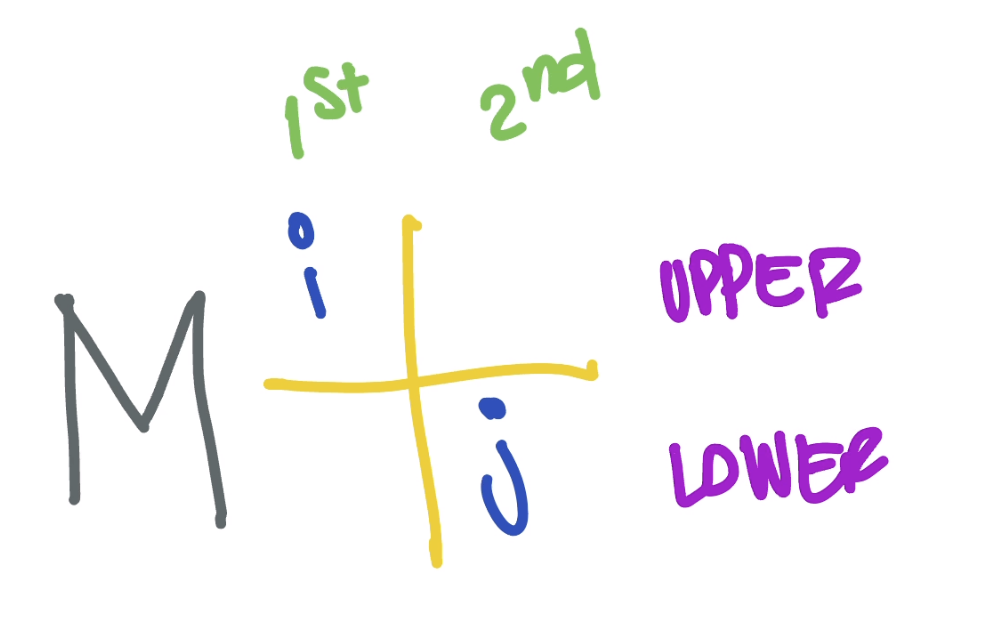
\includegraphics[width=.7\textwidth]{figures/Mij_indices.png}
    \captionsetup{font={scriptsize,sf}}
    \caption{The index placement for a matrix.}
    \label{fig:Mij:index:heights}
\end{marginfigure}
You can take linear combinations of matrices in the same way you take linear combinations of vectors, as per Rule~\ref{rule:vector:linear:combinations}. That is, given two matrices $M$ and $N$, the $ij$-component of the sum of these matrices is
\begin{align}
    (M+N)\aij{i}{j} = M\aij{i}{j} + N\aij{i}{j} \ .
\end{align}
The extension to linear combinations (including rescaling) is trivial.\sidenote{Trivial is how mathematicians say `obvious.' If this point is not obvious, take a moment to see if there is a better way to think about this.}
\begin{example}
Matrices can also be interpreted as vectors. If the index $i$ can run from $1$ to $N$, then a matrix can be understood as an $N^2$-component object. For $2\times 2$ matrices, we could write
\begin{align}
    \vec{v} = 
    \begin{pmatrix}
        v^1 & v^2 \\
        v^3 & v^4
    \end{pmatrix} \ .
\end{align}
In this way, it is a weird repackaging of a 4-component vector. You can check that you can take linear combinations of these `vectors' to form other vectors in the usual way. In this way, the matrix is a repackaging of the components of a vector. Of course, these `vectors' are \emph{completely different} from the 2-component vectors that the $2\times 2$ matrices act on. This identification is rather silly at this point. However, it plays a role in what is called representation theory: the mathematical description of symmetries.
\end{example}

The index structure of matrices means it can contract with both upper-indexed objects like vectors and lower-indexed objects like row vectors. This can happen in several ways. Suppose you have a matrix $M\aij{i}{j}$:
\begin{itemize}
    \item If you also have a row vector $w_i$ and a column vector $v^i$, then you can form a number by contracting them together in the only allowed way: $w_i M\aij{i}{j}v^j$.
    \item If you have a column vector $v^i$, then you can form another column vector by contracting them in the only allowed way: $M\aij{i}{j}v^j$. Observe that this object has one free\sidenote{Here free means uncontracted.} upper index so that it is a column vector.
    \item If you have a row vector $w^i$, then you can form another row vector by contracting them in the only allowed way: $w_iM\aij{i}{j}$. Observe that this object has one free lower index so that it is a row vector.
    \item If you only have the matrix $M\aij{i}{j}$, you can form a number by contracting its two indices, $M\aij{i}{i}$. This is called the \textbf{trace}\index{trace} of the matrix.
\end{itemize}
You can easily understand the first three contractions from your intuition using the matrix multiplication language of Section~\ref{sec:matrix:multiplication},
\begin{align}
    \row{w} M \vec{v} &= 
    \begin{pmatrix}
        w_1 & w_2
    \end{pmatrix}
    \begin{pmatrix}
        M\aij{1}{1} & M\aij{1}{2}\\
        M\aij{2}{1} & M\aij{2}{2}
    \end{pmatrix}
    \begin{pmatrix}
        v^1 \\ v^2
    \end{pmatrix}
    =  
    w_i M\aij{i}{j} v^j
    \\
    \row{w} M &= 
    \begin{pmatrix}
        w_1 & w_2
    \end{pmatrix}
    \begin{pmatrix}
        M\aij{1}{1} & M\aij{1}{2}\\
        M\aij{2}{1} & M\aij{2}{2}
    \end{pmatrix}
    =  
    \begin{pmatrix}
        w_i M\aij{i}{1} & w_i M\aij{i}{2}
    \end{pmatrix}
    \\
    M\row{v} &= 
    \begin{pmatrix}
        M\aij{1}{1} & M\aij{1}{2}\\
        M\aij{2}{1} & M\aij{2}{2}
    \end{pmatrix}
    \begin{pmatrix}
        v^1 \\ v^2
    \end{pmatrix}
    =  
    \begin{pmatrix}
        M\aij{1}{i}v^i \\ M\aij{2}{i}v^i
    \end{pmatrix} \ .
\end{align}
But here we see something powerful about the index notation: in matrix notation, it \emph{does not} make sense to act on a row vector with a matrix `from the right,'
\begin{align}
    M\row{w} = ? \ .
\end{align}
However, from an index point of view:
\begin{align}
    M\aij{i}{j}w_i = w_i M\aij{i}{j} \ .
\end{align}
This is because $M\aij{i}{j}$ is not the matrix $M$, it is a specific \emph{component} of the matrix $M$. As such, it is just a number and multiplication of numbers is commutative.\sidenote{I refer back to Section~\ref{sec:treachery:of:indices:vi:is:not:a:vector}.} Similarly,
\begin{align}
    M\aij{i}{j}v_j = v_j M\aij{i}{j} \ ,
\end{align}
and
\begin{align}
    w_i M\aij{i}{j}v_j = v_j w_i M\aij{i}{j} = v_j  M\aij{i}{j} w_i \ ,
\end{align}
and so forth. This is not `breaking' anything. In fact, our indexology rules are highlighting that it is the matrix multiplication language of Section~\ref{sec:matrix:multiplication} that is limited. 

We re-iterate once more:
\begin{newrule}[Contracted indices] The type of object (tensor) that you have after performing an contraction is determined by the leftover \emph{uncontracted} indices.
\end{newrule}
This means that the trace, $M\aij{i}{i}$ is a number because it has no free (uncontracted) indices. It also means that a matrix acting on a vector $M\aij{i}{j}v^j$ is a vector because it has one free upper index. Of course, we can also imagine other types of objects that return something different when contracting with a vector.

\paragraph{Matrix multiplication} In terms of index notation, matrix multiplication is the contraction of the upper index of one matrix with the lower index of the other. If we multiply matrices $M$ and $N$ in that order, then the $i$--$j$ component of the product is:
\begin{align}
    (MN)\aij{i}{j} =   M\aij{i}{k} N\aij{k}{j}  = N\aij{k}{j} M\aij{i}{k} \ .\label{eq:multiplication:MN:indices}
\end{align}
The second equality here is simply a statement that the product of \emph{numbers} is commutative. Explicitly for the two dimensional case:
\begin{align}
    (MN)\aij{i}{j} &= 
    M\aij{i}{1} N\aij{1}{j} + M\aij{i}{2} N\aij{2}{j}\\
    &=
    N\aij{1}{j} M\aij{i}{1}  + N\aij{2}{j} M\aij{i}{2} \ .
\end{align}
Be sure to read this carefully. Equation \eqref{eq:multiplication:MN:indices} does \emph{not} mean that matrix multiplication is commutative, in particular:
\begin{align}
    N\aij{k}{j} M\aij{i}{k} \neq (NM)\aij{i}{j} \ .
\end{align}
\begin{exercise}
Write out $(NM)\aij{i}{j}$ and confirm that the index contractions are \emph{not} the same as $N\aij{k}{j} M\aij{i}{k}$.
\end{exercise}
What should we make of all this? When we write $MN$ we are implicitly using the matrix multiplication convention of Section~\ref{sec:matrix:multiplication}. Thus $MN$ is \emph{different} from $NM$, as you can check by expanding out the indices.\sidenote{Please do this for a pair of $2\times 2$ matrices if this is not yet clear.} However, index notation tells us that in the expression for a \emph{component of}, $MN$, that is, in $(MN)\aij{i}{j}$, each term in the sum is simply made up of a product of numbers. That product is commutative. 

To say all this differently: matrix multiplication a~la  Section~\ref{sec:matrix:multiplication} told us that there are two different ways to multiply matrices $M$ and $N$: $MN$ and $NM$. In index notation, we also have two different ways to multiply matrices:
\begin{align}
    M\aij{i}{k}N\aij{k}{j}
    &&\text{and}&&
    M\aij{k}{j}N\aij{i}{k} = N\aij{i}{k}M\aij{k}{j} \ .
\end{align}
These two different index contractions correspond to $MN$ and $NM$ respectively.\sidenote{If this is making you scratch your head or exhale with a deep sigh of ennui, it may help to know that matrix multiplication is still an active field of computational mathematics research.\footnotemark}\footnote{\url{https://www.quantamagazine.org/ai-reveals-new-possibilities-in-matrix-multiplication-20221123/}}



\begin{newrule}[From matrix multiplication to index contraction and back]\label{rule:matrix:multiplication:to:indices:and:back}
To convert from the matrix multiplication picture---where matrices are $N\times N$ blocks of numbers that act on columns according to Figure~\ref{fig:matrix:col:mult}---to index notation: first write out all objects with explicit indices. Matrix multiplication corresponds to the contraction of consecutive indices, for example $A\vec{v} = A\aij{i}{j}v^j$. Once you have written everything in terms of indices, you can move factors around: $A\aij{i}{j}v^j = v^jA\aij{i}{j}$ because there is no ambiguity which indices are contracted.

To go from index notation back to matrix multiplication, arrange all contractions so that they are consecutive and interpret consecutive contractions as matrix multiplications. For example:
\begin{align}
     A\aij{i}{j}v_j  w_i =
     w_i A\aij{i}{j} v_j = \row{w} A \vec{v} 
     = 
     \begin{pmatrix}
         w_1 & w_2 
     \end{pmatrix}
     \begin{pmatrix}
         A\aij{1}{1} & A\aij{1}{2}\\
         A\aij{2}{1} & A\aij{2}{2}
     \end{pmatrix}
     \begin{pmatrix}
         v^1\\
         v^2
     \end{pmatrix}
     \ .
\end{align}
It does not matter if you contract lower indices to upper indices or upper indices to lower indices as you read from left-to-right, only that the indices are consecutive. 

\textbf{Caveats}: sometimes different tensor contractions appear to give the same matrix multiplication. Usually in these cases the type of contraction is formally not allowed in the limited matrix multiplication picture. For example, $w^iv^j g_{ij}$ is a valid tensor contraction involving two vectors and an object with two lower indices. It cannot be written as a matrix multiplication without breaking the rules.
\end{newrule}



\paragraph{Matrix inverses}
We touched on inverse matrices in \eqref{eq:matrix:invers:multiplcation:notation}. Let us return to it using index notation. \emph{If} a matrix is invertible, then the condition \eqref{eq:matrix:invers:multiplcation:notation} is
\begin{align}
    M\aij{i}{k}(M\inv)\aij{k}{j} = (M\inv)\aij{i}{k}M\aij{k}{j} = \delta^i_j
    \label{eq:index:matrix:inverse}
\end{align}
where we define the Kronecker-$\delta$,\sidenote{The Kronecker-$\delta$ are the components of the identity matrix. Because it is diagonal, the order of the indices does not matter so we can write both indices with the same horizontal alignment. In a contraction, the Kronecker-$\delta$ simply says: replace a sum over one of my indices with the value of the other index.}
\begin{align}
    \delta^i_j = \begin{cases}
    1 & \text{if } i=j \\
    0 & \text{otherwise .}
    \end{cases}
    \label{eq:kronecker:delta}
\end{align}
If the indices can take values from 1 to $N$, then there are $N^2$ equations to constrain the $N^2$ components of $M\inv$. If the matrix $M$ is invertible, then one could solve this system of equations to determine $M\inv$. In silly versions of this course, one would spend time using some software---perhaps Matlab---to solve this system of equations. That's silly. Matrices are either invertible by hand, easy to invert using your favorite computer algebra system\sidenote{\emph{Mathematica} is popular among theorists, though \emph{NumPy} and \emph{SciPy} are both open source.}, or so hopelessly impossible to invert that other techniques are needed to approximate their inversion.\sidenote{Taylor expansions about an easier-to-invert matrix, for example.} However, understanding what it means to invert a matrix is a \emph{big} part of mathematical physics. In fact, it is a central thrust of physics.
\begin{bigidea}\label{idea:matrix:inverse:in:physics}
A surprisingly large swath of physics---and certainly the part that is most do-able---boils down to inverting matrices of various (often infinite) sizes. This is because equations in physics are often in the form
\begin{align}
    (\text{operator})\, \ket{\text{state}} = \ket{\text{source}} \ .
\end{align}
We have used ket notation, but recall that these are just vectors. Usually you know what the operator (matrix) is and you know what the source is. For example, the operator may be some vector calculus operator, perhaps the divergence. The source is usually a physical configuration, perhaps the density of charge. Then the state---which is what you want to find---would be the electric field. The general solution to problems in this form is
\begin{align}
 \ket{\text{state}} = (\text{operator})\inv\, \ket{\text{source}} \ .
\end{align}
And it thus behooves us to understand what it means to invert an operator. So another way to think about our course, ``linear algebra for physicists,'' is to say it is the toolkit to invert operators that show up in physics.
\end{bigidea}

\subsection{Tensors}
\label{sec:index:tensors:rotation:on:each:index}

A \textbf{tensor}\index{tensor} is an object with some number of ordered indices. Each index has a definite height. We say that a tensor is a $(p,q)$ tensor if it has $p$ upper indices and $q$ lower indices. Vectors, row vectors, and matrices are all tensors. We met an example of a different type of tensor in Figure~\ref{fig:Riemann:tensor:for:indices}, the Riemann tensor,\sidenote{In general relativity (differential geometry) this tensor takes in three vectors and returns another vector. The first two vectors are sides of a parallelogram. In a general curved space, one cannot close this parallelogram. If we take the third vector and `transport it' along the two paths of the parallelogram, the difference in what happens to the third vector is what the Riemann tensor returns. See Figure~\ref{fig:Penrose:14:10:Riemann}.} $R^i_{\phantom{i}jk\ell}$. What can this object do? 
\begin{marginfigure}%[th]
    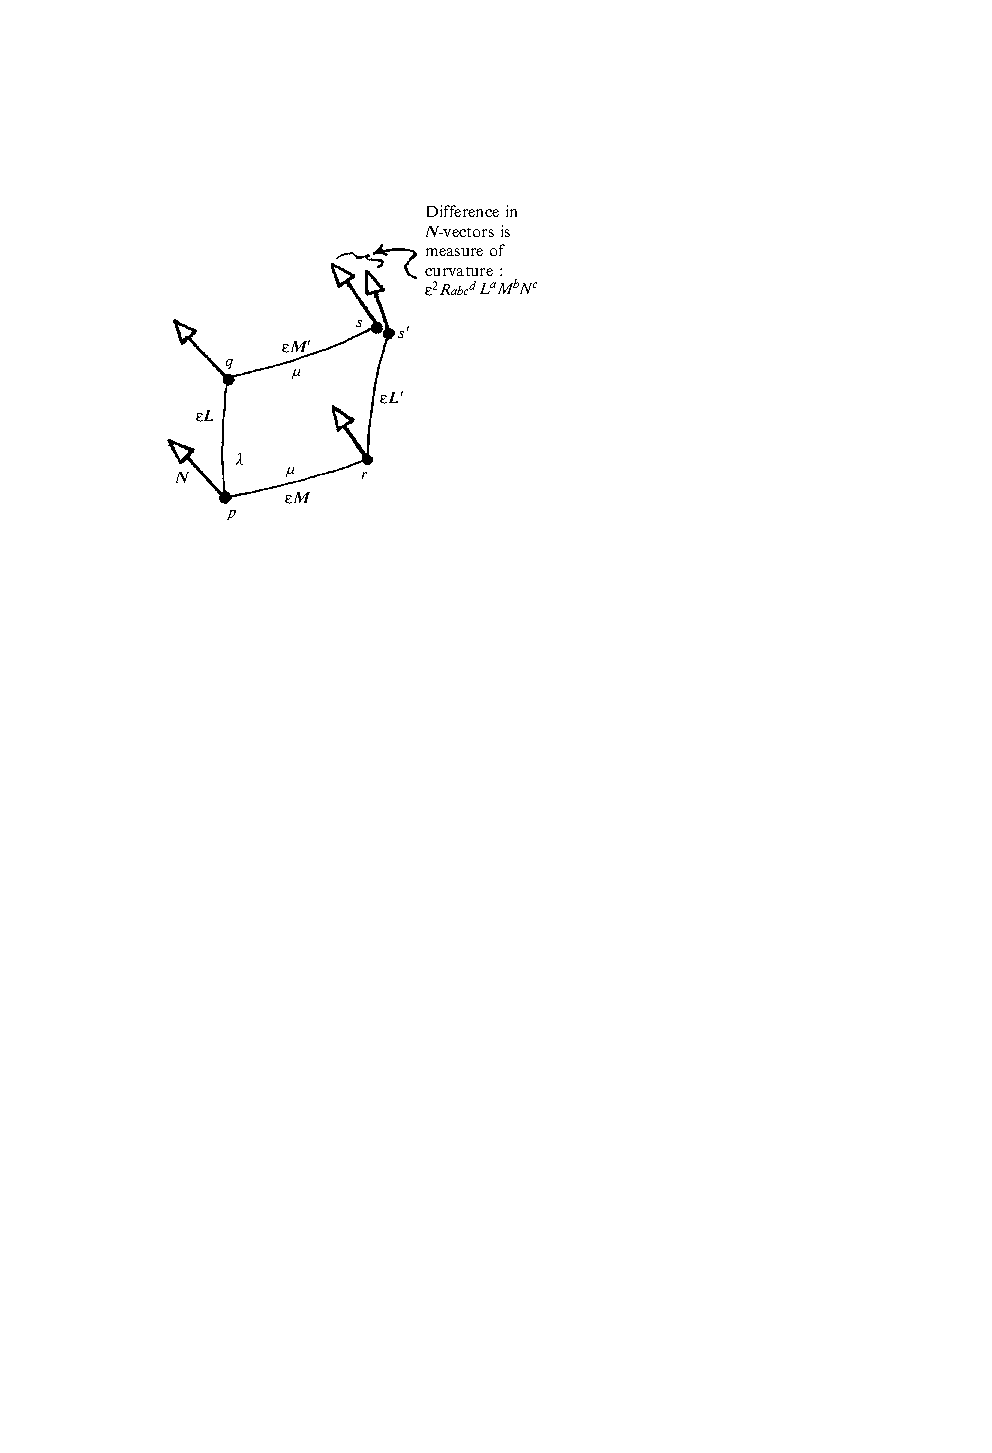
\includegraphics[width=.8\textwidth]{figures/Penrose_Riemann_14_10.pdf}
    \captionsetup{font={scriptsize,sf}}
    \caption{Graphical depiction of what the Riemann tensor from Penrose, \emph{Road to Reality}. Note that Penrose uses a different ordering of indices than we do.}
    \label{fig:Penrose:14:10:Riemann}
\end{marginfigure}
Based on the index structure alone, you can determine that the Riemann tensor can:
\begin{itemize}
    \item Take three vectors and a row vector to return a number, $R^i_{\phantom{i}jk\ell} v^jw^ku^\ell t_i$.
    \item Take two vectors and return a matrix, $R^i_{\phantom{i}jk\ell}v^kw^\ell$. 
    \item Take two vectors and a row vector to return a row vector, $R^i_{\phantom{i}jk\ell}w_iv^ju^k$.
    \item ... and a few more that you can write out. Do not forget contractions of the upper index with one of the lower indices.
\end{itemize}
\begin{newrule}[Tensor contractions]
A $(p,q)$ tensor can contract with $r\leq p$ row vectors and $s \leq q$ column vectors to produce a $(p-r, q-s)$ tensor. By allowing `traces' of the tensor's own upper and lower indices, you can also produce $(p-r-n, q-s-n)$ tensors so long as $p-r-n\geq 0$ and $q-s-n\geq 0$.
\end{newrule}
\begin{exercise}
You can generalize the above rule by allowing a $(p_1,q_1)$ tensor to contract with a $(p_2, q_2)$ tensor. Write out some of the ways in which a $(2,2)$ tensor can contract with a $(1,3)$ tensor. Here is one example: $T^{ij}_{\phantom{ij}k\ell} S^\ell_{\phantom{\ell}ijm}$. 
\end{exercise}
You can see that tensor contraction can get a little dicey. There is a cute graphical notation called birdtracks notation to keep track of this that never became popular.\sidenote{The cover image for these notes is an example of one such contraction. You can learn more about this in Penrose's \emph{Road to Reality}.} In this course we do not worry about very complicated contractions and can stick to index notation.


\subsection{A prelude to symmetry}
\label{sec:isometry:first:pass:indices}
Some ideas are so significant that we introduce them multiple times. Let us preview a key idea: an \textbf{isometry}\index{isometry} is a special symmetry that some vector spaces may have.\sidenote{Specifically, vector spaces equipped with an inner product---called metric spaces---may have isometries.} Let us not concern ourselves for now with the conditions for when such symmetries exist. Instead, for this first pass let us say that isometries are generalizations of rotations.  Take a moment to review the `matrix multiplication' picture of rotations in Section~\ref{sec:Euclidean:three:space:rotations}: rotations $R$ satisfy $R^\trans R = \one$ and, due to this, they preserve the angle and length of vectors. The preservation of angle and length depend on a definition of the dot product---and we are not doing that just yet. However, we can take the lesson that the dot product takes vectors and creates scalars.\sidenote{Scalar is a fancy name for number. More practically, scalars do \emph{not} change under rotations.}

We know that one way to form numbers from objects that have indices is to contract all available indices. Let us examine the simplest such case: a row vector whose indices are contracted with a column vector: $w_iv^i$. Rotations are transformations that act on both row vectors and column vectors. Because row and column vectors are two separate classes of tensorial objects, we allow for the possibility that row vectors and column vectors transform differently:
\begin{align}
    v^i &\to v'^i \defeq R\aij{i}{j}v^j & w_i &= \to w'_j\defeq w_j \tilde{R}\aij{j}{i} \ ,
    \label{eq:components:of:vector:and:row:under:rotatino}
\end{align}
where $R$ and $\tilde{R}$ are the matrices that encode the linear transformation on vectors and row vectors respectively.\sidenote{Neither of these have anything to do with the Riemann curvature tensor, which unfortunately is denoted with an $R$.} We write $v'^i$ and $w'_j$ to be the components of the rotated $v^i$ and $w_j$. Inspired by our earlier intuition that rotations should preserve the value of `fully contracted' objects,\sidenote{All tensor indices are contracted, no free indices.} we can demand that
\begin{align}
    w_i v^i =w'_i v'^i = R\aij{i}{j}v^j \, w_k\tilde{R}\aij{k}{i}
    =\tilde{R}\aij{k}{i}R\aij{i}{j} w_kv^j \ .
    \label{eq:rotations:index:preserve:inner:product:01}
\end{align}
Let us do something silly. We would like to `do algebra' on this equation, which means I would like to cancel out common factors on each side. I would like to cancel the $w_i$ and $v^i$ on the left with the $w_kv^j$ on the right. I can relabel dummy indices,\sidenote{By `dummy index' I mean contracted indices where the choice of variable name does not matter. Though every time I say `dummy index' I think about the `dummy plug' program in \emph{Neon Genesis Evangelion}.} but we need to break apart the fact that $w_i$ and $v^i$ have the same index on the left-hand side. To do this, we multiply by one using the Kronecker-$\delta$: $w_iv^i = w_i \delta^i_j v^j$. Then we may rewrite  \eqref{eq:rotations:index:preserve:inner:product:01} as
\begin{align}
    \cancel{w_i} \cancel{v^j}  \delta^i_j
    =\tilde{R}\aij{i}{\ell}R\aij{\ell}{j} \cancel{w_i} \cancel{v^j} \ ,
\end{align}
from which we have simply:
\begin{align}
    \tilde{R}\aij{i}{\ell}R\aij{\ell}{j} &= \delta^i_j \ .
    \label{eq:R:Rtilde:transformation:from:indices:rotation}
\end{align}
Comparing to \eqref{eq:index:matrix:inverse}, we see that this is the statement that $\tilde R = R\inv$. We have come to a key observation:
\begin{quote}
Under a rotation, an object with an upper index transforms with some matrix $R$ that encodes the rotation. An object with a lower index then transforms with the inverse matrix, $R\inv$. In this way, when a row vector and column vector have their indices contracted, they produce a number that is \emph{invariant} (unchanged) under rotations.
\end{quote}
This observation actually generalizes:
% 
\begin{newrule}[Transformation of upper and lower indices under rotations]
\label{idea:transformation:of:upper:and:lower:indices}
Under an isometry (such as a rotation) $R$, a tensorial object transforms as follows
\begin{align}
    T\aij{i_1\cdots i_N}{j_1\cdots j_M}
    \to 
    R\aij{i_1}{k_1}\cdots R\aij{i_N}{k_N}
    (R\inv)\aij{\ell_1}{j_1}\cdots (R\inv)\aij{\ell_M}{j_M}
    T\aij{k_1\cdots k_N}{\ell_1\cdots \ell_M} \ .
    \label{eq:transformation:of:upper:and:lower:indices}
\end{align}
That is to say: each upper index is contracted with a rotation $R$ and each lower index is contracted with an inverse rotation $R\inv$. 
\end{newrule}

\begin{exercise}
Show that for the case of $2\times 2$ rotations, the inverse is equivalent to the transpose. This turns out to be true for any rotation matrix in Euclidean space.
\end{exercise}

\begin{exercise}
Show that our rule for how row vectors transform can be written in matrix notation as:
\begin{align}
    \row{w} \to \row{w}' \equiv \row{w} R^\trans \ .
\end{align}
To do this, show that the index contracts correspond to the right-hand side. Use the result of the previous exercise that $R\inv = R^\trans$ for rotations.
In this way, it is clear that $\row{w}\vec{v} = \row{w'}\vec{v'}$ is invariant under rotations:
\begin{align}
    \row{w'}\vec{v'} = \row{w}R^\trans R\vec{v} = \row{w} \one \vec{v} \ ,
\end{align}
where we use the definition \eqref{eq:RTR:one}.
\end{exercise}





\section{Vector Space}

If you have some vectors, the combined set of all possible linear combinations of those vectors is called a \textbf{vector space}. This is the idea introduced in Section~\ref{sec:linear:combination:and:span}. Suppose you have some vectors\sidenote{Note that the lower index here is \emph{not} a component index! The vector $\vec{v_2}$ has components $(v_2)^1, (v_2)^2, \cdots$.},  $\vec{v}_1, \cdots, \vec{v}_N$. From these vectors, you can form an infinite number of other vectors by choosing numbers $\alpha^i$ and forming the linear combination
\begin{align}
    \alpha^1 \vec{v}_1 + \alpha^2\vec{v}_2 + \cdots + \alpha^N \vec{v}_N \ .
    \label{eq:linear:combination:looks:like:basis}
\end{align}
The set of all possible vectors that can be formed this way is called the \textbf{vector space} \emph{spanned by}  $\vec{v}_1, \cdots, \vec{v}_N$. The word \textbf{span}\index{span} means the vector space of all linear combinations of a set of vectors. When we say that \emph{linear combinations of vectors are also vectors}, what we mean is that they are \emph{also vectors in the vector space}. We write vector spaces with a capital letter, say $V$, and write that a vector $\vec{v}$ is part of the vector space by writing
\begin{align}
    \vec{v} \in V \ .
\end{align}

\begin{example}
If you have two vectors,
\begin{align}
    \vec{v} &= 
    \begin{pmatrix}
        3 \\ 1 \\ 0
    \end{pmatrix}
    &
    \vec{w} &= 
    \begin{pmatrix}
        2 \\ 1 \\ 3
    \end{pmatrix}
    \label{eq:eg:of:vector:space:1}
\end{align}
then you could form another vector that is a linear combination of the two:
\begin{align}
    2\vec{v} - 1 \vec{w}
    =
    \begin{pmatrix}
        4 \\ 1 \\ -3
    \end{pmatrix} \ .
\end{align}
We say that this vector is part of the vector space $V$ spanned by $\vec{v}$ and $\vec{w}$. 
\end{example}

\begin{example}
If $V$ is the vector space spanned by by $\vec{v}$ and $\vec{w}$ in \eqref{eq:eg:of:vector:space:1}, then the vector
\begin{align}
    \vec{u}
    =
    \begin{pmatrix}
        3 \\ 1 \\ 2
    \end{pmatrix} \ .
\end{align}
is \emph{not} part of the vector space $V$ because there are no coefficients $\alpha^1$ and $\alpha^2$ that can satisfy
\begin{align}
    \alpha^1\vec{v} + \alpha^2 \vec{w} = \vec{u} \ .
\end{align}
If you are not convinced, please try it. In the above condition, how many unknowns are there? How many component-level constraint equations are there?
\end{example}

\begin{example}
Consider the vectors
\begin{align}
    \vec{a}
    &=
    \begin{pmatrix}
        1\\0
    \end{pmatrix}
    &
    \vec{b}
    &=
    \begin{pmatrix}
        0\\1
    \end{pmatrix}
    &
    \vec{c}
    &=
    \begin{pmatrix}
        1\\1
    \end{pmatrix}\ .
\end{align}
The vector space spanned by these three vectors is \emph{all} of the two-component vectors. In fact, the vector space spanned by any \emph{two} of these vectors is all of the two-component vectors. 
\end{example}


By this notion of duality, you should expect that row vectors also form a vector space. If the space of column vectors is called $V$, then the space of row vectors is called $V^*$. Evidently there is some relation between the two, even though they appear be totally different vector space.\sidenote{That is: we could have just said that row vectors live in a vector space $W$ and $W$ has nothing to do with $V$.} Indeed, the relation is that that row vectors can contract with column vectors. The star evidently means the space of \emph{vectors that can contract with this other set of vectors}. In this way, column vectors are the dual space of row vectors: $(V^*)^* = V^{**} = V$. This is simply saying that in the contraction $w_i v^i$, we can think of $w_i$ acting on $v^i$ or we can equivalently think of $v^i$ acting on $w_i$. 


\section{Basis of a Vector Space}\label{sec:basis}

Let us return to \eqref{eq:linear:combination:looks:like:basis}. Take a moment to take a good look at that equation. In fact, this equation is so important that we write it out again:
\begin{align}
    \alpha^1 \vec{v}_1 + \alpha^2\vec{v}_2 + \cdots + \alpha^N \vec{v}_N \ .
    \tag{\ref{eq:linear:combination:looks:like:basis}}
\end{align}
Here are a few thoughts that may come to your mind while looking at this linear combination of vectors.
\begin{enumerate}
    \item Hmm. We have $N$ vectors and took a linear combination of them. This means that we needed $N$ coefficients. Rather than writing $\alpha$, $\beta$, $\gamma$, and so forth, we chose to jsut label them all $\alpha$ but with an upper index. 
    \item Oh... the upper index is convenient because it means we can write the linear combination as $\alpha^i \vec{v}_i$. But this isn't a ``real'' contraction, right? Well... it follows the summation convention so I suppose that's legitimate. It is just weird that $\vec{v}_i$ is an entire vector with and additional lower index.
    \item In fact, these $\alpha^i$ coefficient look suspiciously like the components of a vector.
    \item Wait a second, $\alpha^i\vec{v}_i$ \emph{is} a vector.
    \item Can I think about $\alpha^i$ as being the components of the vector $\alpha^i\vec{v}_i$?
\end{enumerate}


\subsection{An understanding between friends}
This brings us to the critical idea of a basis. Now is a good time to go over the examples in the previous section. Go ahead and do that. \emph{Right now.} Okay, welcome back. Suppose that you and I agreed on a set of vectors. Let's say that we both agreed on the $N$ vectors in \eqref{eq:linear:combination:looks:like:basis}; we even agree on the numbering. Let us call this special set of vectors a \textbf{basis}\index{basis}. That means that if I want to communicate to you some linear combination of those vectors, all I have to do is give you a list of their coefficients. I would write this as a column,
\begin{align}
    \vec{a} = 
    \begin{pmatrix}
        \alpha^1\\
        \vdots \\
        \alpha ^N
    \end{pmatrix} \ .
\end{align}
You may say: oh, that's an odd way to write a linear combination---just stacking the coefficients in a column like that. But sure, we both understand that what this \emph{really} means is
\begin{align}
    \vec{a} = 
    \alpha^i \vec{v}_i \ ,
\end{align}
we can just leave the $\vec{v}_i$ implicit because we both already agree on what those vectors are. 

Maybe you see what is going on here. We previously introduced vectors as columns of numbers. Now we are saying that columns of numbers represent a particular linear combinations of basis vectors. It seems that all this time, the `column of numbers' that we started actually mean a linear combination of a specific choice of basis vectors. In fact, the standard or canonical basis vectors can be thought of as columns:
\begin{align}
    \bas{e}_1 &= 
    \begin{pmatrix}
        1\\ 0 \\  0 \\\vdots
    \end{pmatrix}
    &
    \bas{e}_2 &= 
    \begin{pmatrix}
        0 \\ 1 \\  0 \\\vdots
    \end{pmatrix}
    &
    \bas{e}_3 &= 
    \begin{pmatrix}
        0 \\ 0 \\  1 \\\vdots
    \end{pmatrix}
    &
    \cdots
    \label{eq:canonical:basis}
\end{align}
We have moved to a notation where we write the basis vectors as $\bas{e}_i$. A basis does not \emph{need} to be nice. 


In terms of the canonical basis \eqref{eq:canonical:basis}, we now understand that the components of a vector mean
\begin{align}
    \vec{v} = v^1 \bas{e}_1 + v^2 \bas{e}_2 + \cdots = v^1 \bas{e}_1 \ .
\end{align}

\begin{bigidea}[The big deal about bases]\label{idea:reasons:to:like:bases}
This whole hubbub about bases is useful for at least two reasons:
\begin{enumerate}
    \item This notion completely abstracts away the \emph{meaning} of a vector. The basis vectors carry all the `vector-ness'\sidenotemark of the vector. 
    \item If you and I are \emph{not} using the same basis, then all I have to do is convert your basis into my basis to be able to convert your components into my components.
\end{enumerate}
\end{bigidea}\sidenotetext{Or more generally, tensor-ness.}

We briefly introduce these two ideas in turn. But first, let us address the index structure of the basis.

\paragraph{Why do basis vectors have lower indices?} Previously we said objects with a single lowered index are row vectors. Are basis vectors row vectors? Not quite. In fact, when we talked about tensors, we said that the specific component $T^{i_1\cdots i_N}_{\phantom{{i_1\cdots i_N}}j_1\cdots j_M}$ is just some number. For basis vectors, once we specify $i$, $\bas{e}_i$ is \emph{not} a number: it carries all of the \emph{meaning} of what a vector \emph{is} in whatever context the vector is being used. The basis vector has a lower index because it means we can contract it with the upper index of $v^i$. The resulting object is the vector itself, $\vec{v}$ which carries no indices. If this sounds like philosophical navel gazing, please jump ahead and do Exercise~\ref{ex:fibonacci:space}---it is a rather different example of `vector-ness' than `columns of numbers.'





\subsection{Abstraction}
\label{sec:sub:abstraction:basis}

% In Section~\ref{sec:sub:basis:changing} we saw how making the basis vectors explicit helps us understand how to relate tensors in one reference frame (basis) to another. Recall that there is a second reason in \bigidearef~\ref{idea:reasons:to:like:bases} why basis vectors are helpful: they
Basis vectors help us further let vectors become more abstract.\sidenote{There is an analogy here to the \LaTeX typesetting system. The goal of \LaTeX is to separate content from the under-the-hood work to present that content. For practical purposes, we want to separate components---which are just numbers that we can work with---from underlying mathematical machinery that gives those components meaning.}
%
Another way of saying this is as follows:
\begin{quote}
Vectors are \emph{not} columns of numbers.
\end{quote}
Those numbers are the \emph{components} of a vector. But the \emph{meaning} of a vector depends on the context. In some contexts the vector might be a velocity or a momentum. It may be a unit excitation in the electric field. It may be the spin state of an electron. It may be a solution to the spherical Laplace equation. The magic is that all sorts of \emph{physical} quantities are described by vectors. The basis vectors carry these identities so that we can just work with numerical coefficients that we happen to denote with upper indices and that we sometimes arrange in columns.


\paragraph{Arrow space}
Our goal is to abstract away any notion of column vectors. A useful way to think about this is an idea that is perhaps familiar: imagine vectors are arrows with a magnitude and a direction. The rule for adding vectors is that you stack them together, tail-to-head.\sidenote{It should be clear that this definition is commutative, $\vec{v}+\vec{w} = \vec{w}+\vec{v}$.} For example, consider the following basis:
\begin{align}
    \bas{e}_1 &= \eqfig{
\includegraphics[width=2em]{figures/basis_e1.pdf}}
    &
    \bas{e}_2 &= \eqfig{
\includegraphics[width=2em]{figures/basis_e2.pdf}} \ .
\end{align}
Then a vector $\vec{v}$ may be written as a linear combination of those vectors. Figure~\ref{fig:eg:basis:arrows:canonical:eg} demonstrates this.
\begin{marginfigure}%[th]
    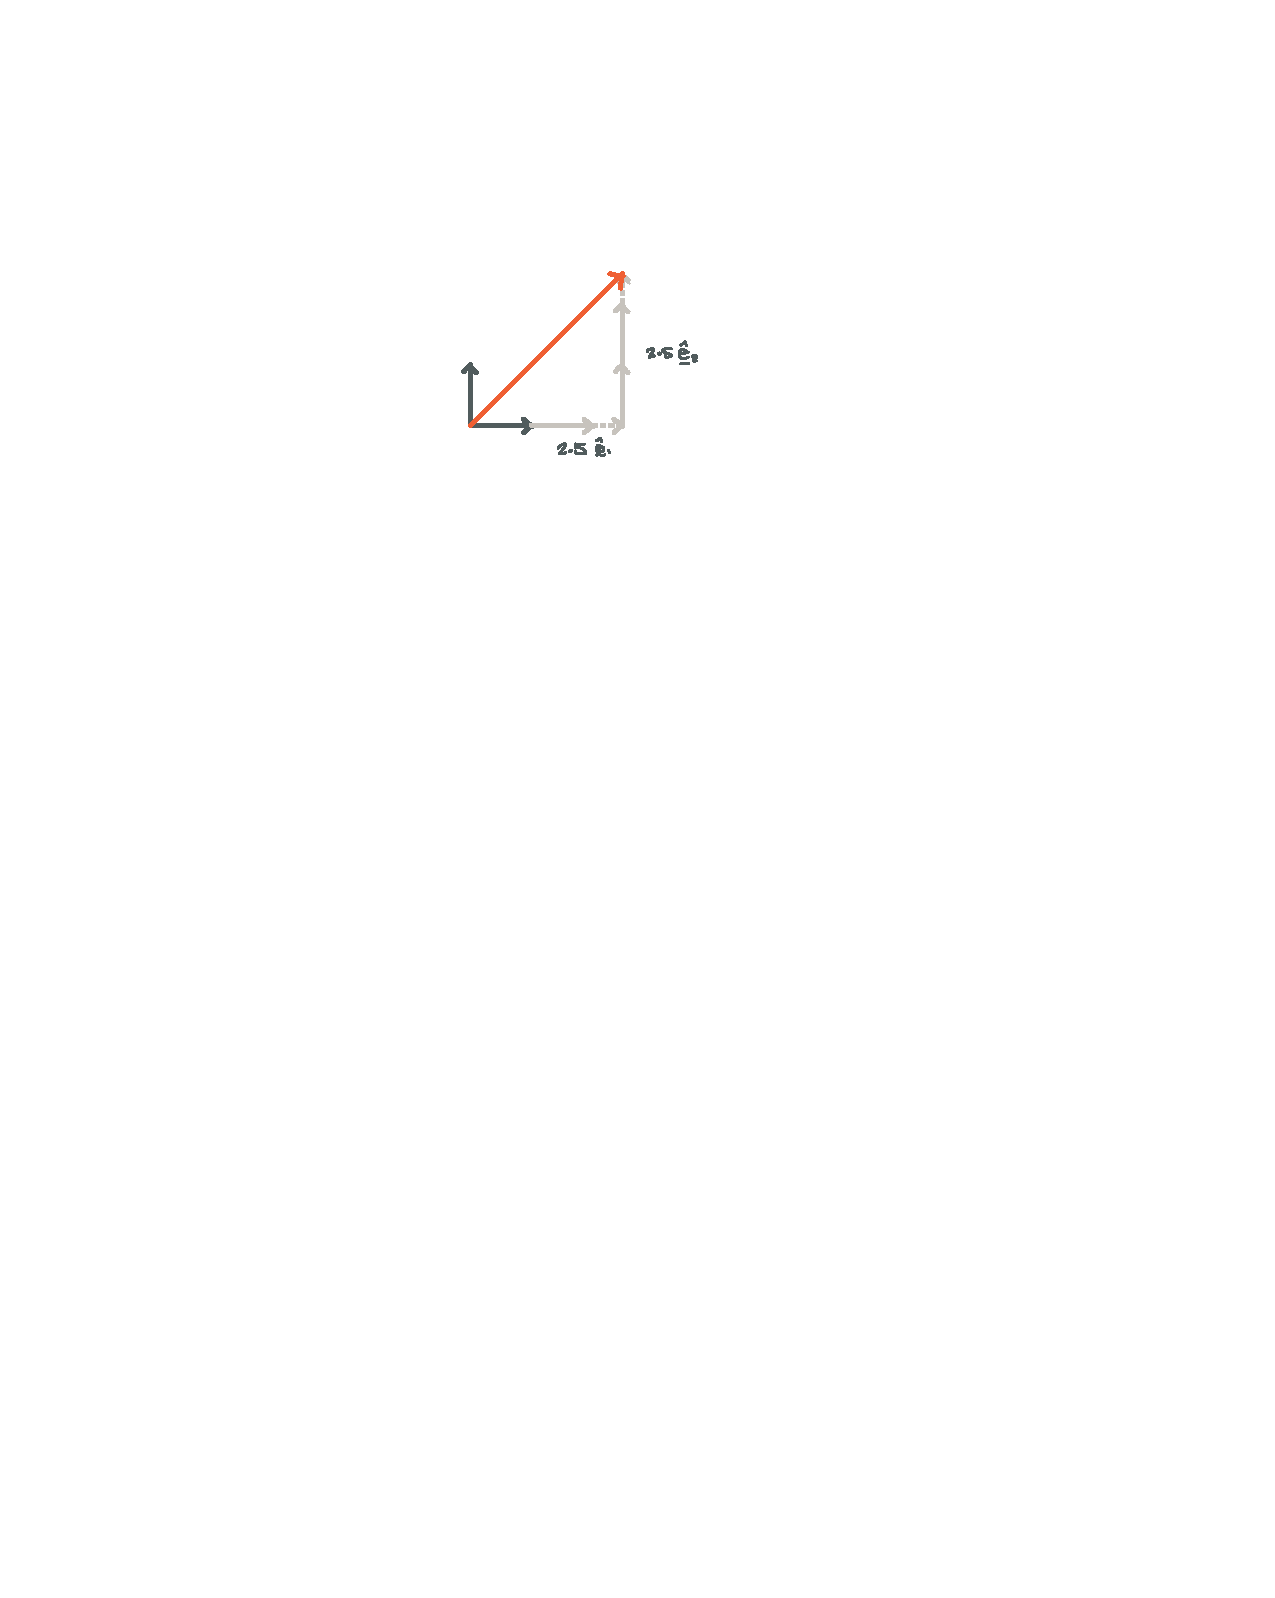
\includegraphics[width=.6\textwidth]{figures/basis_red_e.pdf}
    \captionsetup{font={scriptsize,sf}}
    \caption{The vector $\vec{v}$ (in red) is $2.5\bas{e}_1 + 2.5\bas{e}_2$.}
    \label{fig:eg:basis:arrows:canonical:eg}
\end{marginfigure}
In that example, the components of the vector $\vec{v}$ are
\begin{align}
    \vec{v} &= v^i\bas{e}_i = 2.5 \bas{e}_1 + 2.5 \bas{e}_2  \ .
\end{align}
We could have used a different basis of the same space. This basis is
\begin{align}
    \bas{f}_1 &= \eqfig{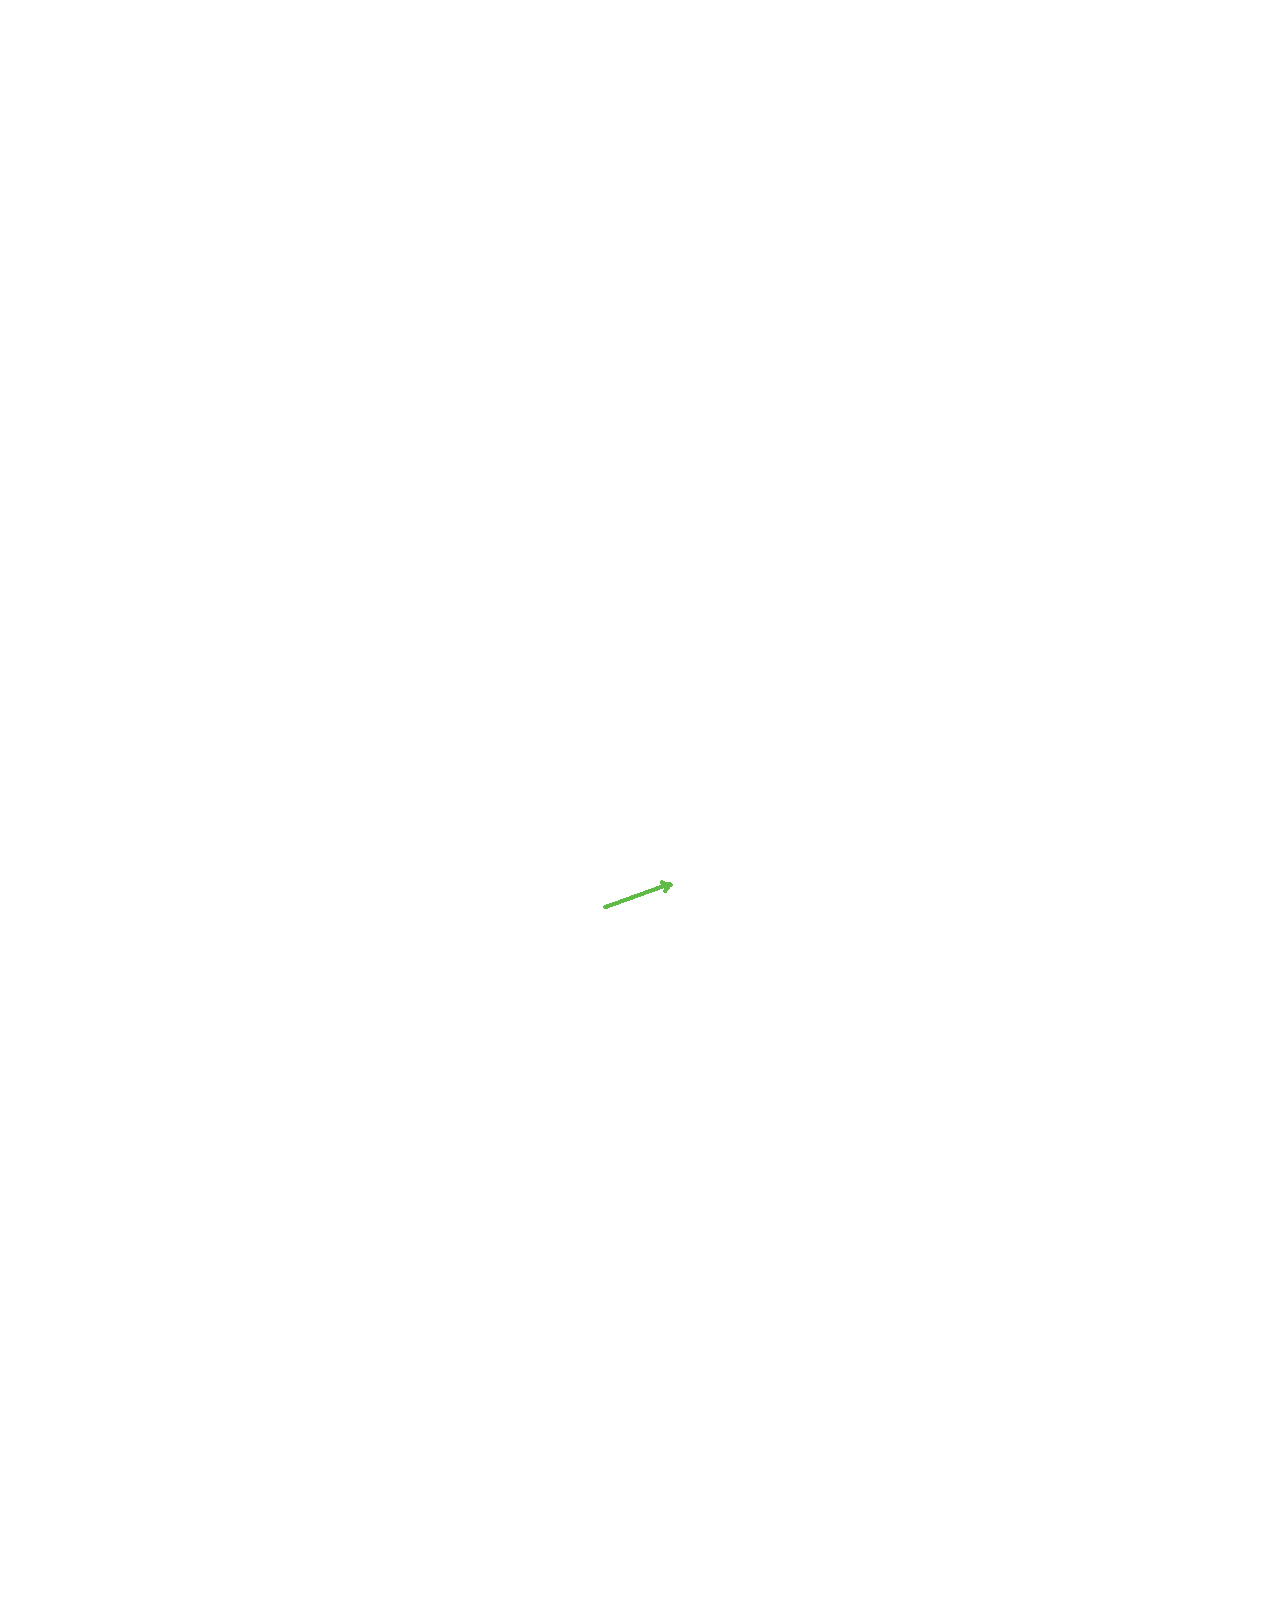
\includegraphics[width=2em]{figures/basisf1.pdf}}
    &
    \bas{f}_2 &= \eqfig{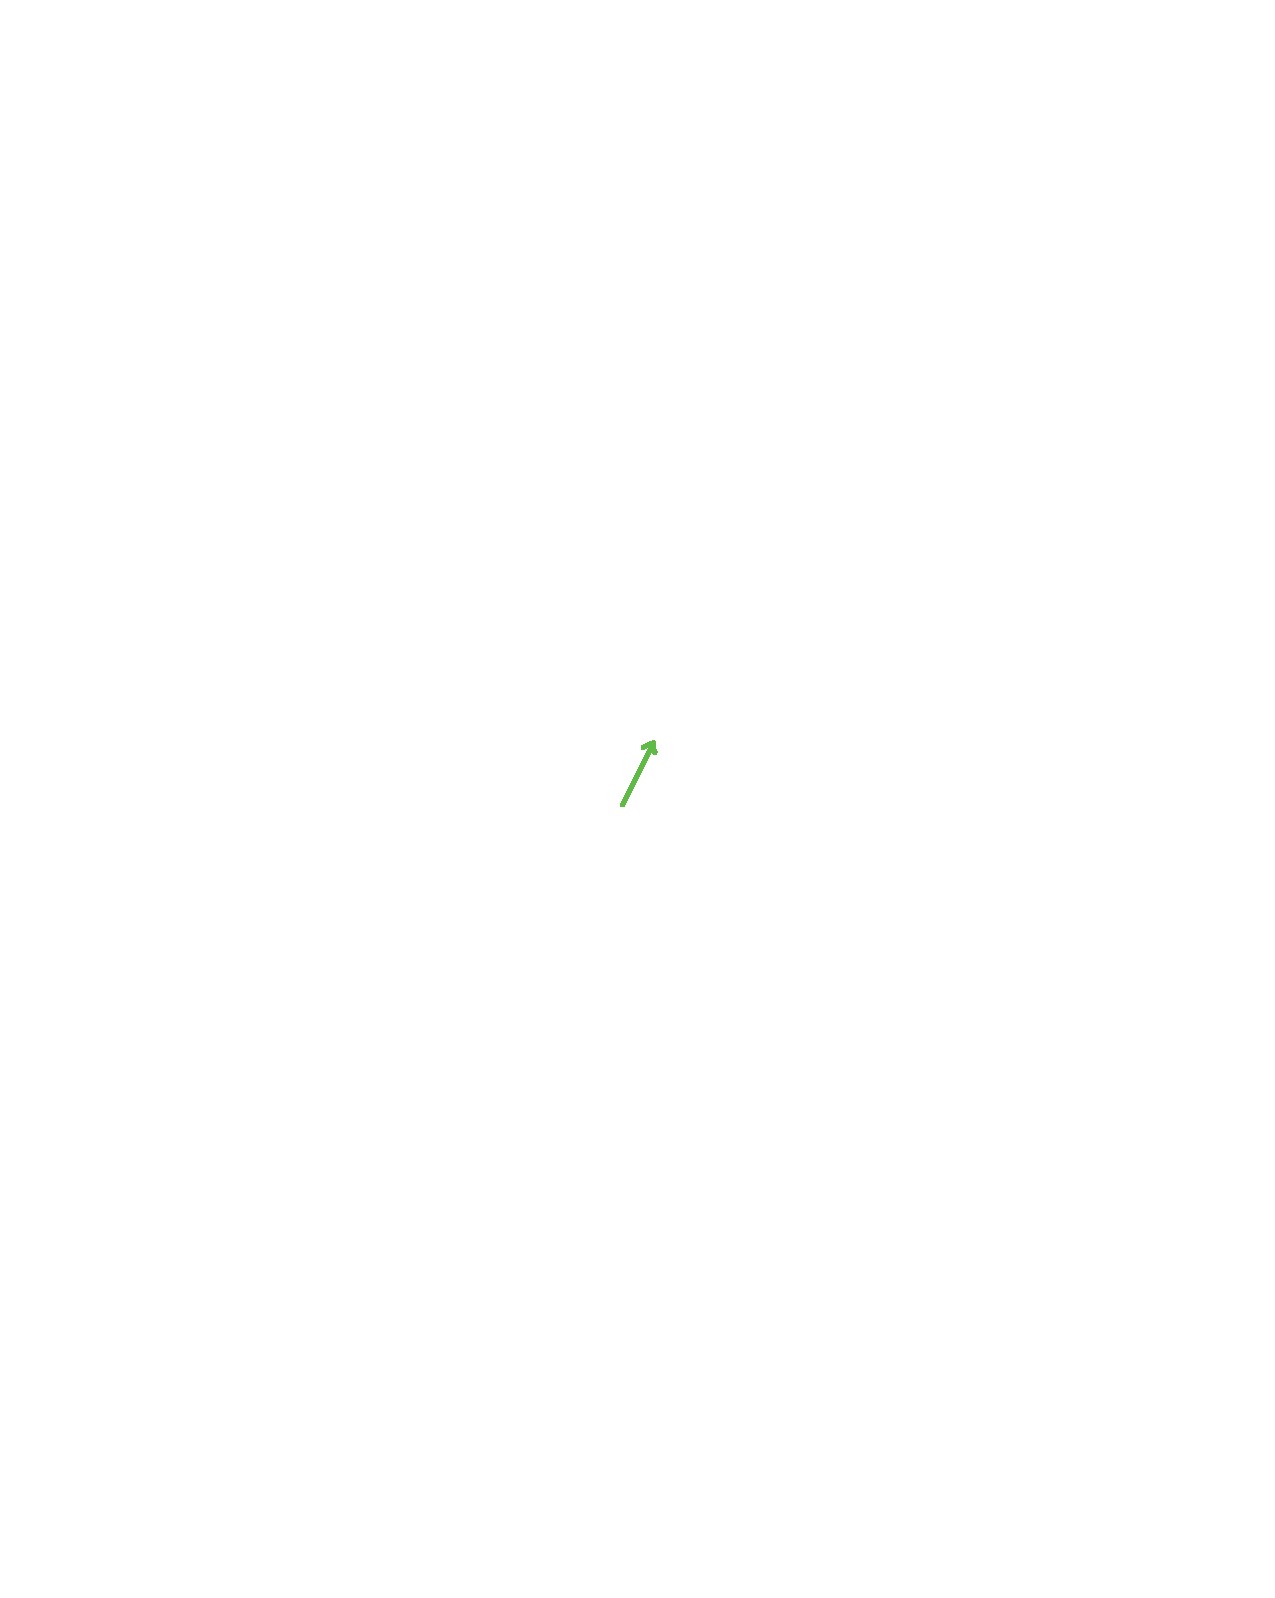
\includegraphics[width=2em]{figures/basisf2.pdf}} \ .
\end{align}
Figure~\ref{fig:eg:basis:arrows:canonical:eg:odd:basis} shows the same vector $\vec{v}$ written as a linear combination of the $\bas{f}_{1,2}$ basis.
\begin{marginfigure}%[th]
    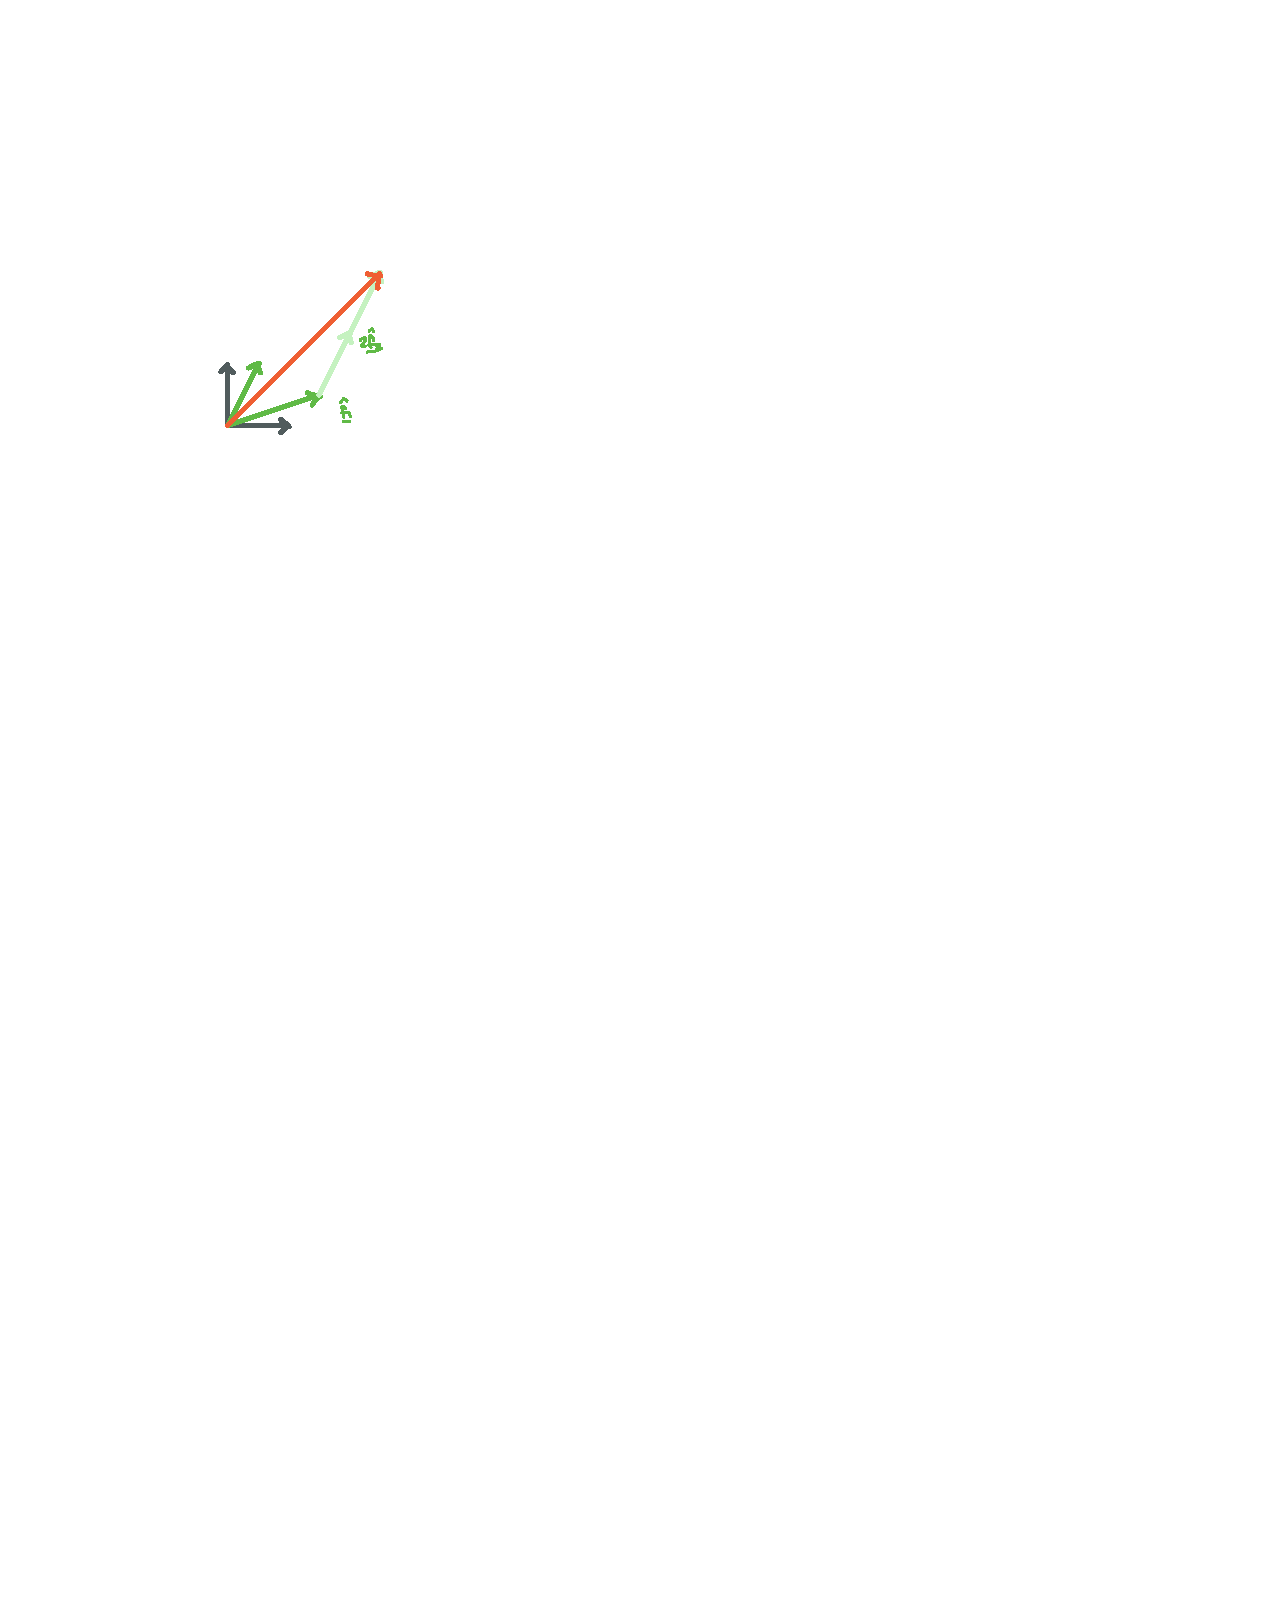
\includegraphics[width=.6\textwidth]{figures/basis_red_f.pdf}
    \captionsetup{font={scriptsize,sf}}
    \caption{The vector $\vec{v}$ (in red) is $\bas{f}_1 + 2\bas{f}_2$.}
    \label{fig:eg:basis:arrows:canonical:eg:odd:basis}
\end{marginfigure}
\begin{align}
    \vec{v} &= v'^i\bas{f}_i =  \bas{f}_1 + 2\bas{f}_2  \ .
\end{align}

As a final demonstration, we illustrate that coefficients of basis vectors may also be negative. In Figure~\ref{fig:eg:basis:arrows:neg} we have a vector in blue that is a positive sum of the $\bas{e}_{1,2}$ basis vectors, but is the linear combination $3\bas{f}_1 - \bas{f}_2$ in the $\bas{f}_{1,2}$ basis.
\begin{marginfigure}%[th]
    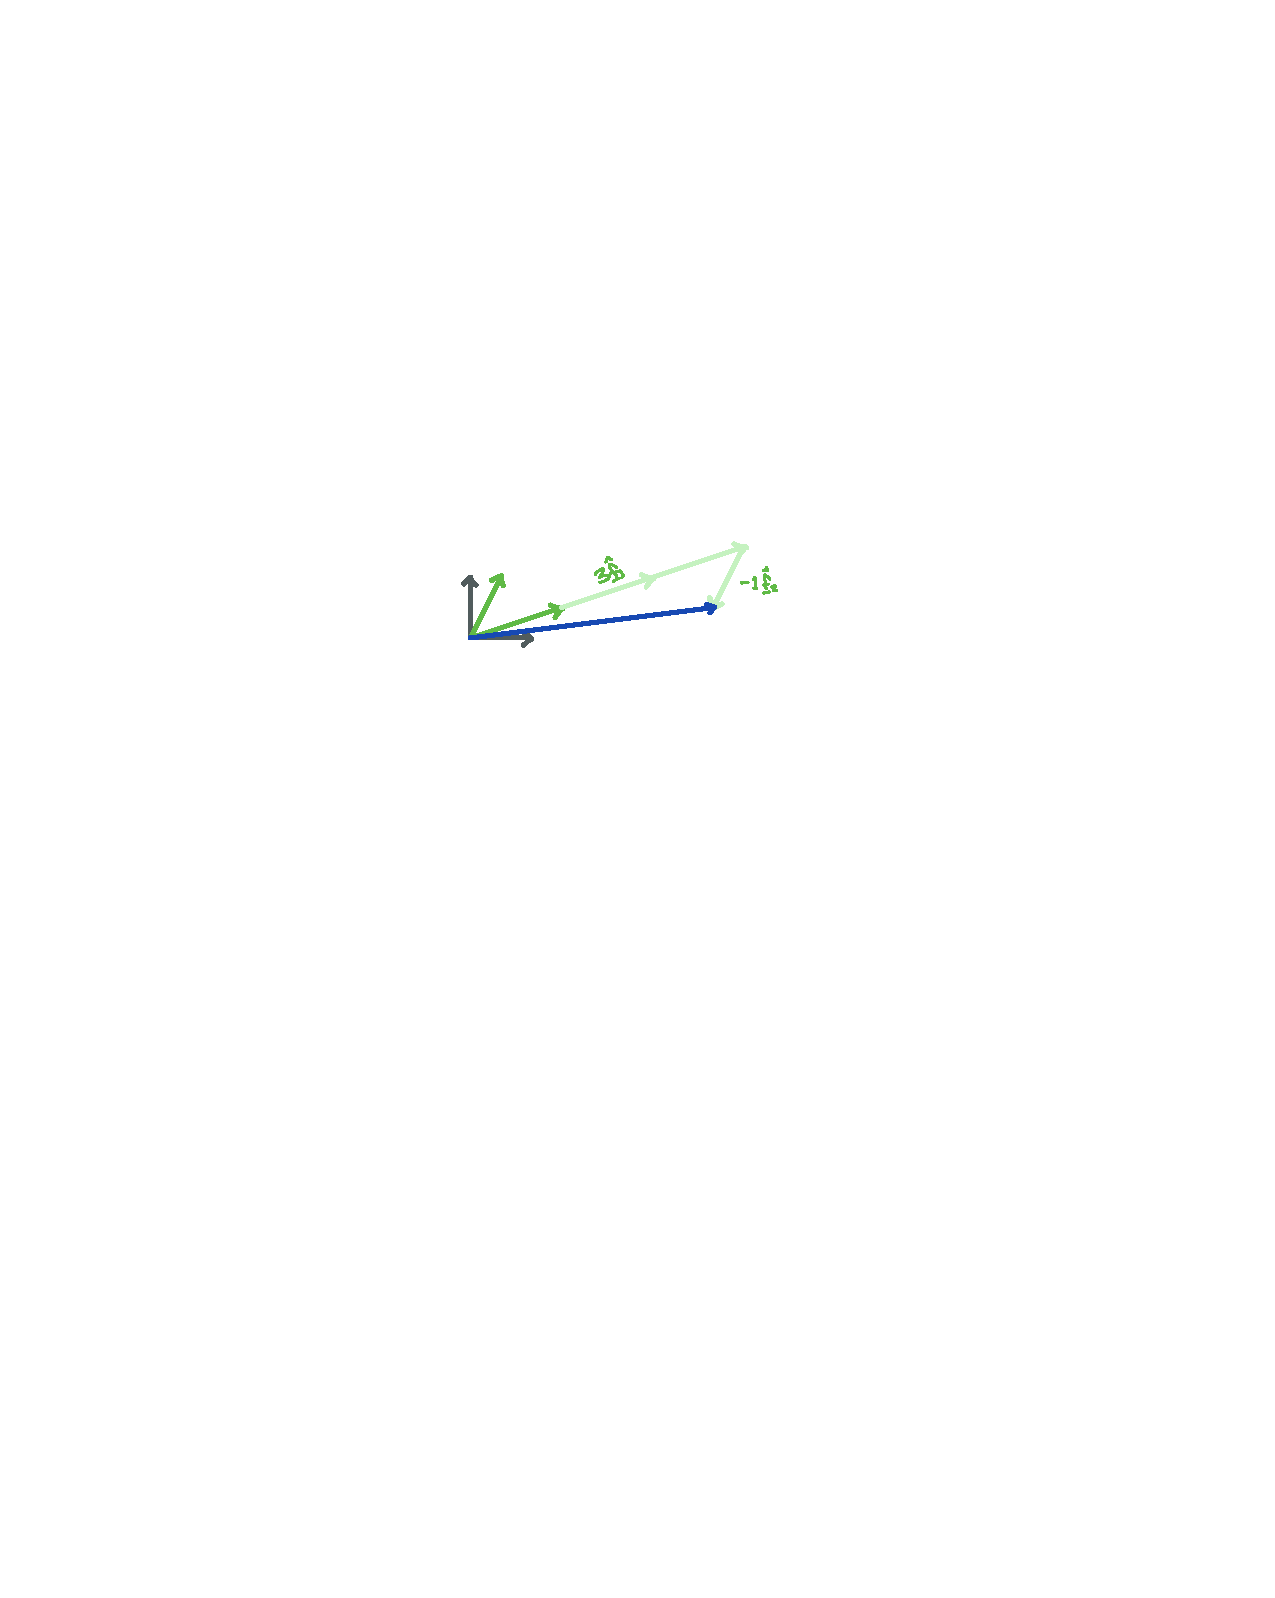
\includegraphics[width=\textwidth]{figures/basis_neg.pdf}
    \captionsetup{font={scriptsize,sf}}
    \caption{Example of a vector (blue) that has a negative coefficient of $\bas{f}_2$ in the $\bas{f}_{1,2}$ basis.}
    \label{fig:eg:basis:arrows:neg}
\end{marginfigure}

\begin{example}\label{ex:cheeseburger:space}
A silly vector space the space spanned by cheeseburgers ($\bas{e}_1$) and fries ($\bas{e}_2$) are your favorite local burger joint:
\begin{align}
\bas{e}_1 &=
    \eqfig{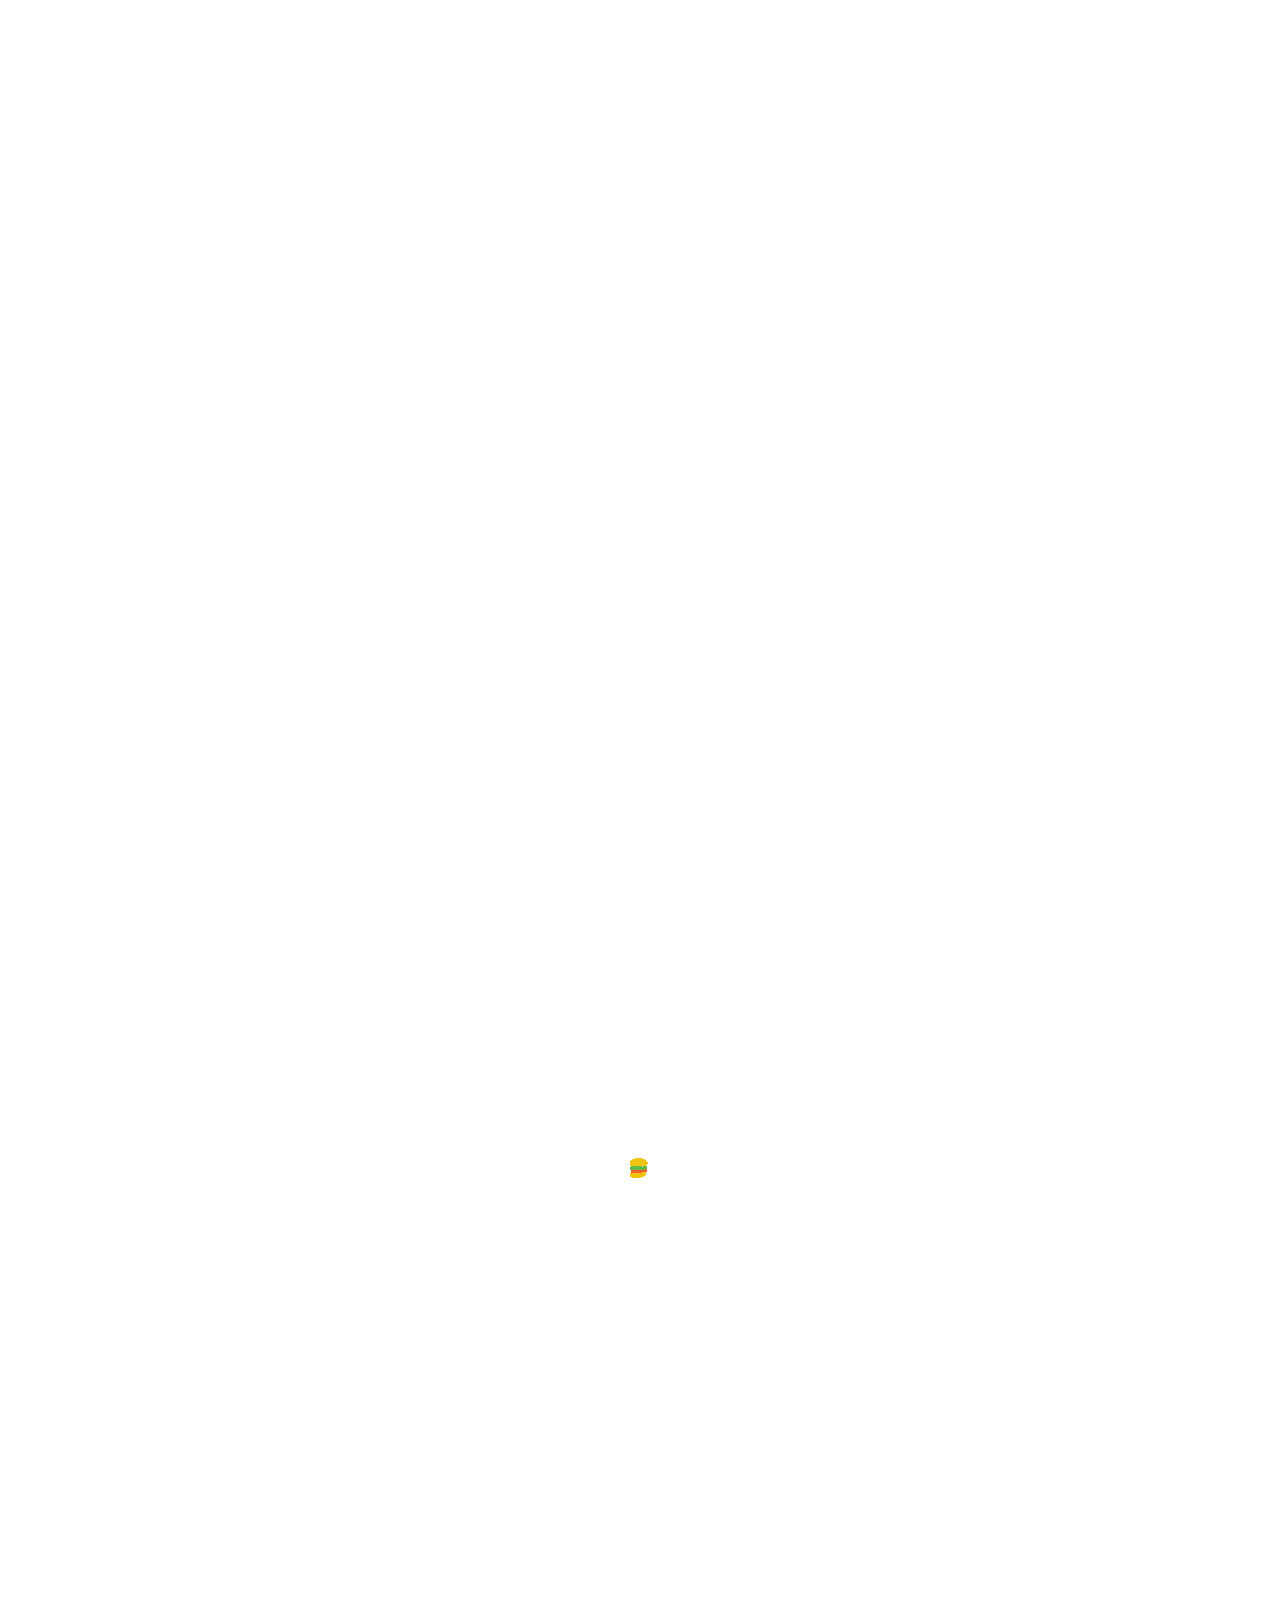
\includegraphics[width=1.5em]{figures/basis_food_icon_burger.pdf}}
    &
    \bas{e}_2 &=
    \eqfig{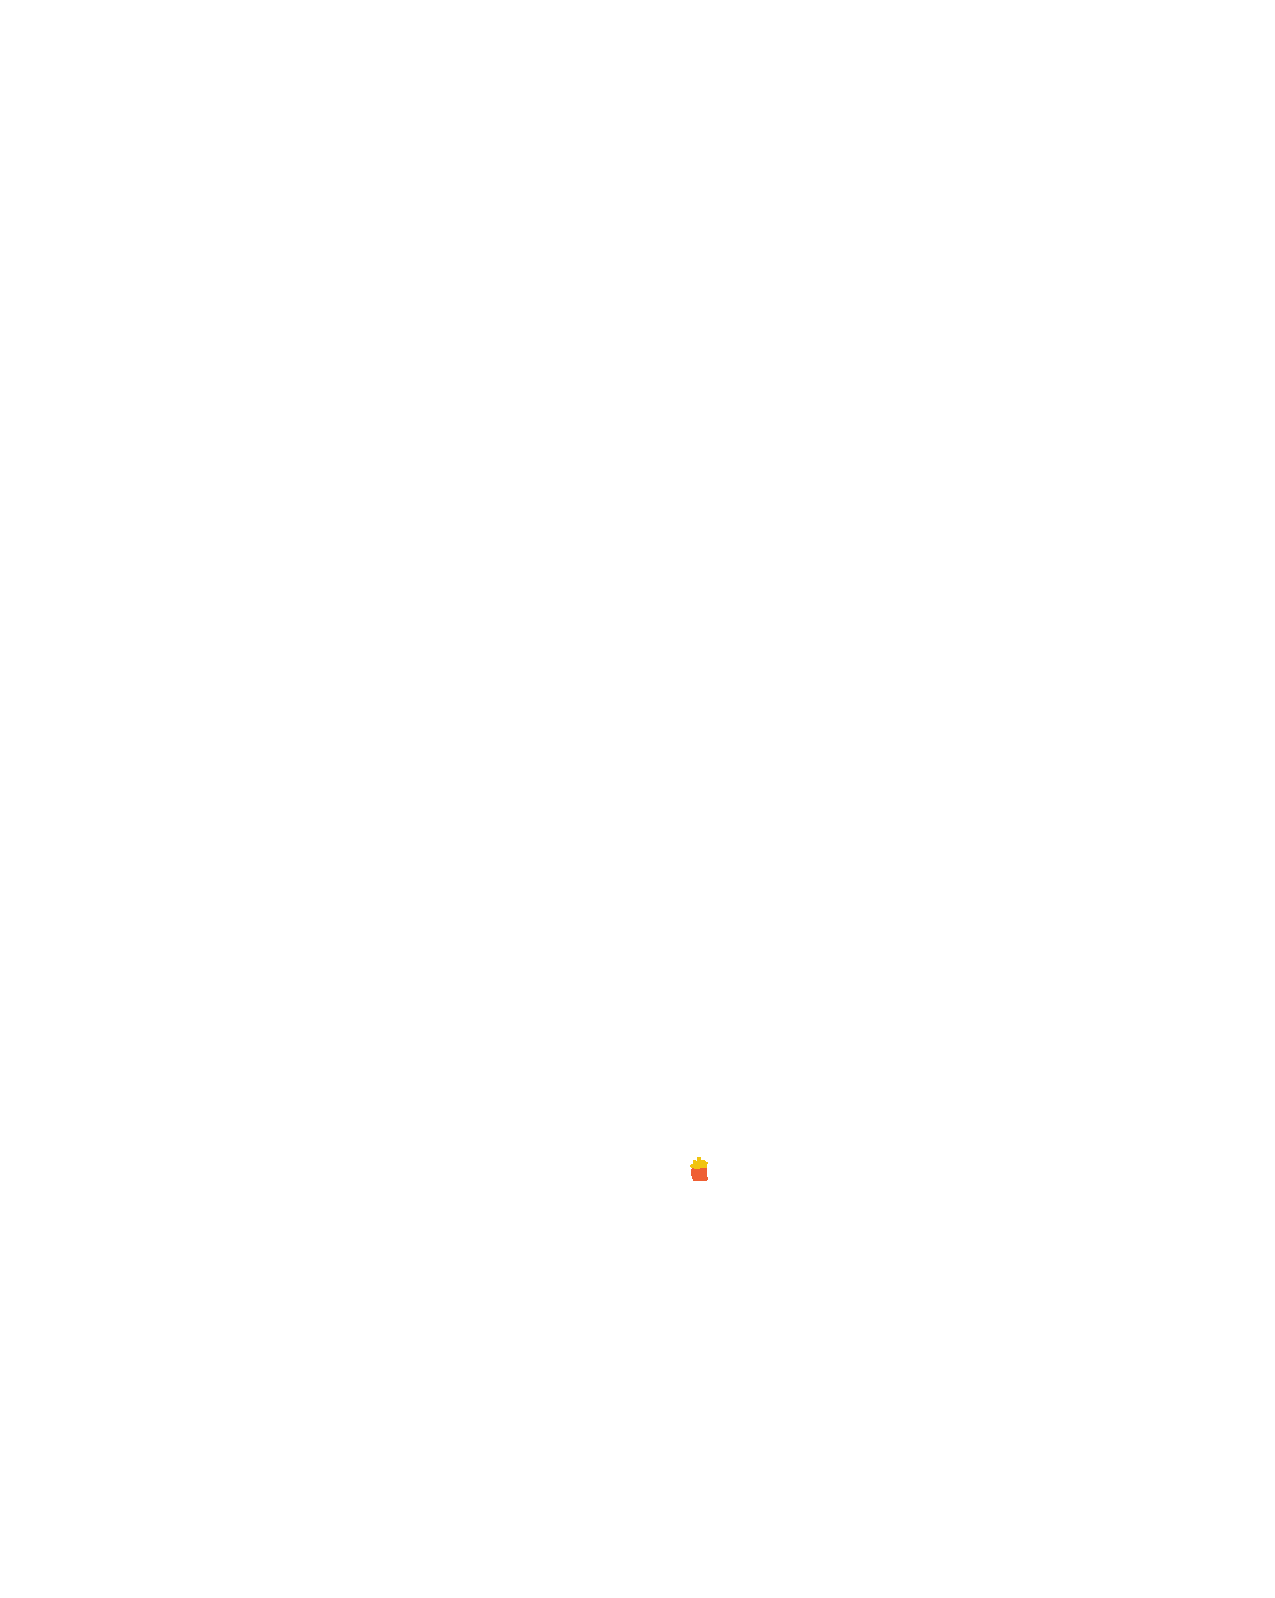
\includegraphics[width=1.5em]{figures/basis_food_icon_fries.pdf}} 
    &
    \eqfig{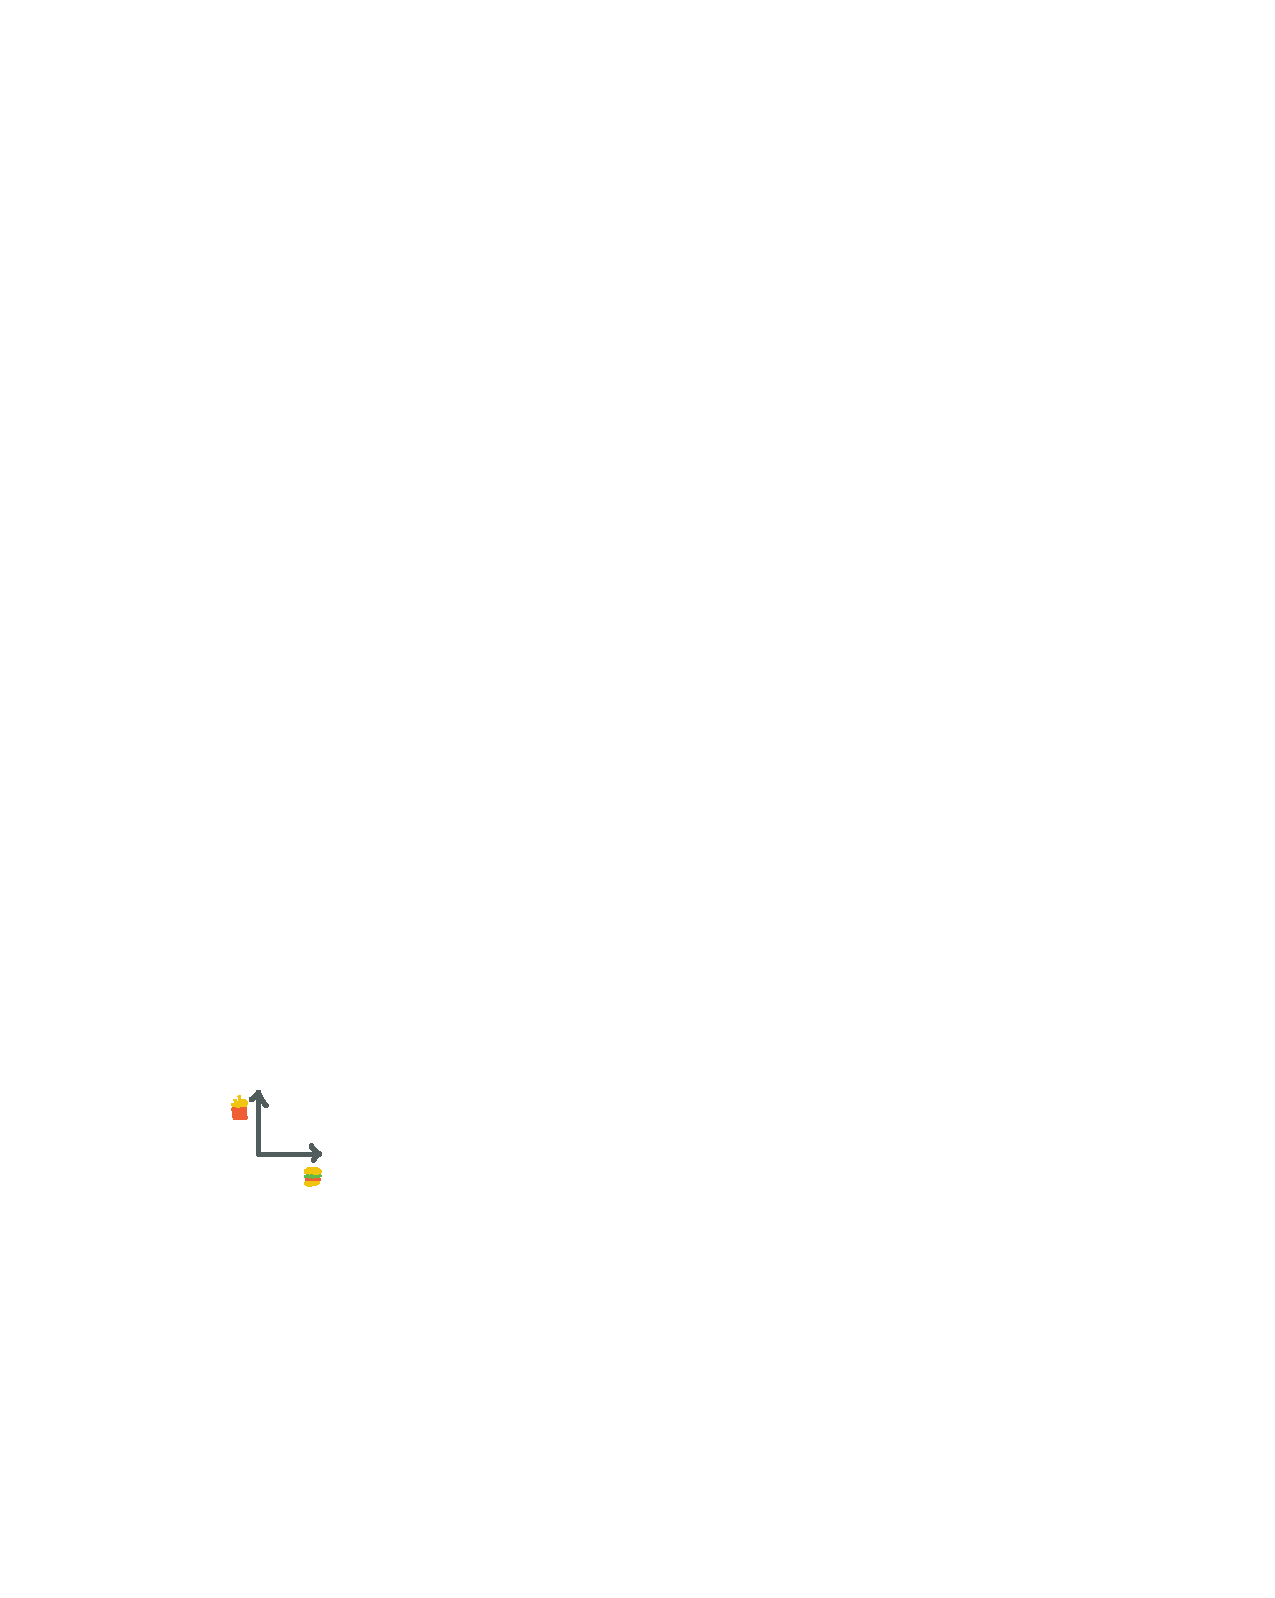
\includegraphics[width=4em]{figures/basis_food_canonical.pdf}} 
    \ .
\end{align}
Then an order $\vec{v}$ of 2 burgers and 1 fries is
\begin{align}
    \vec{v} =
    2\bas{e}_1 + \bas{e}_2 = 
    2\eqfig{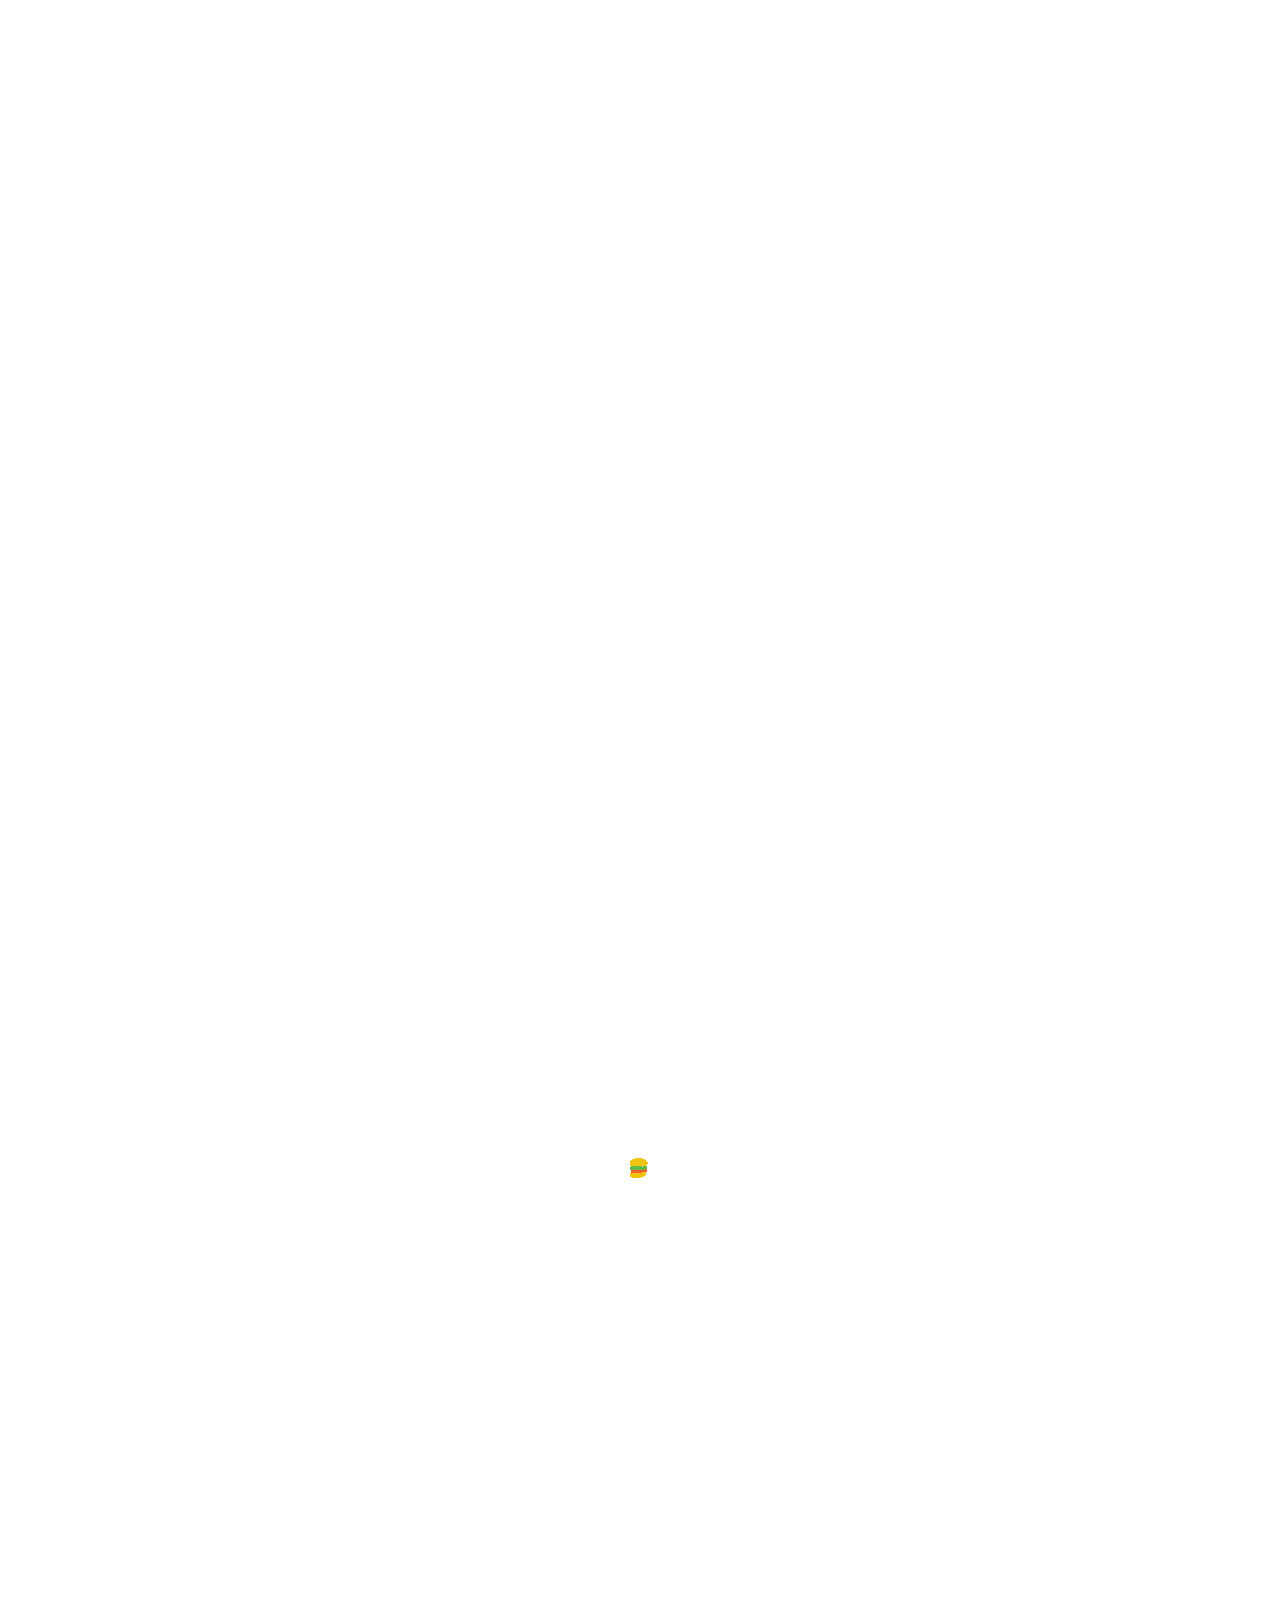
\includegraphics[width=1.5em]{figures/basis_food_icon_burger.pdf}} 
    +
    \eqfig{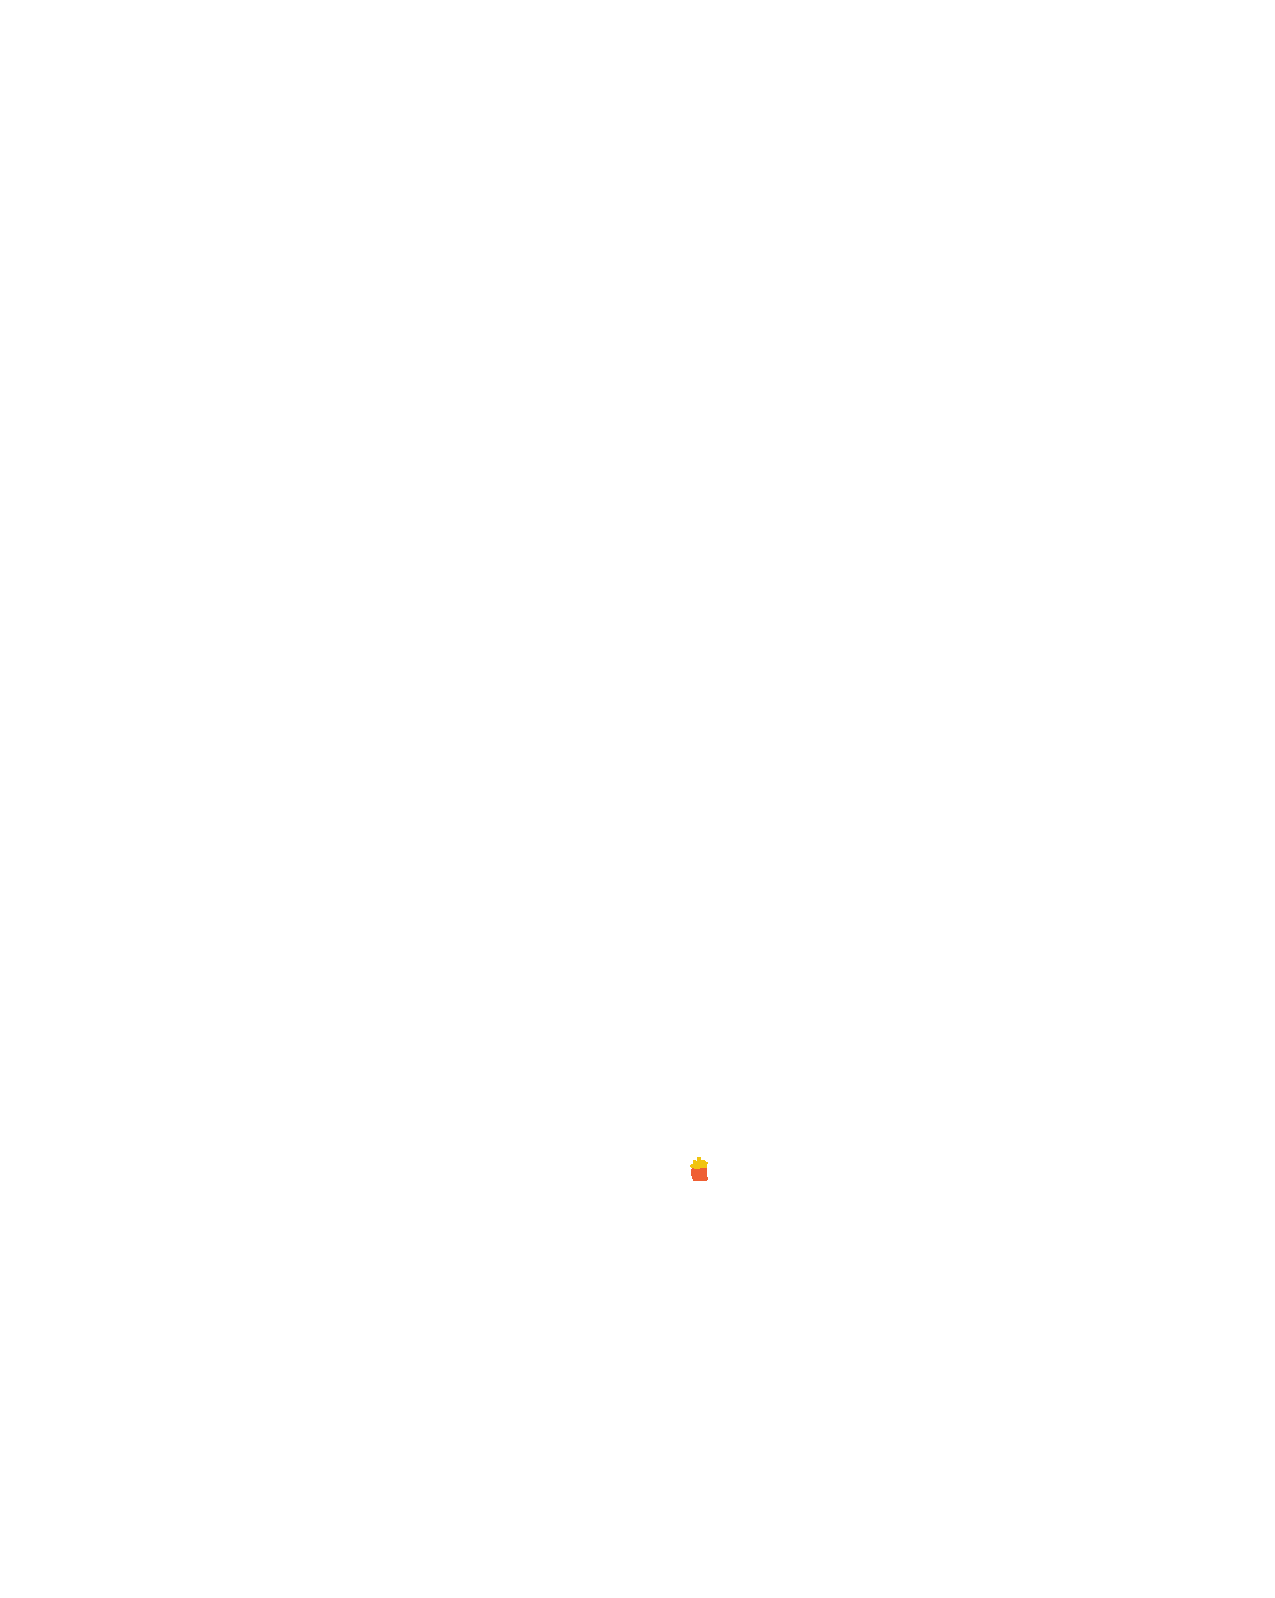
\includegraphics[width=1.5em]{figures/basis_food_icon_fries.pdf}} \ .
    \label{eq:basis:eg:meal:1}
\end{align}
Suppose the burger joint also offers a combo meal that includes one burger and one fries. Then we can choose another basis of combo meals ($\bas{f}_1$) and fries ($\bas{f}_2 = \bas{e}_2$); on the right we show it relative to the other basis:
\begin{align}
\bas{f}_1 &=
    \eqfig{
\includegraphics[width=1.5em]{figures/basis_food_icon_meal.pdf}}
    &
    \bas{f}_2 &=
    \eqfig{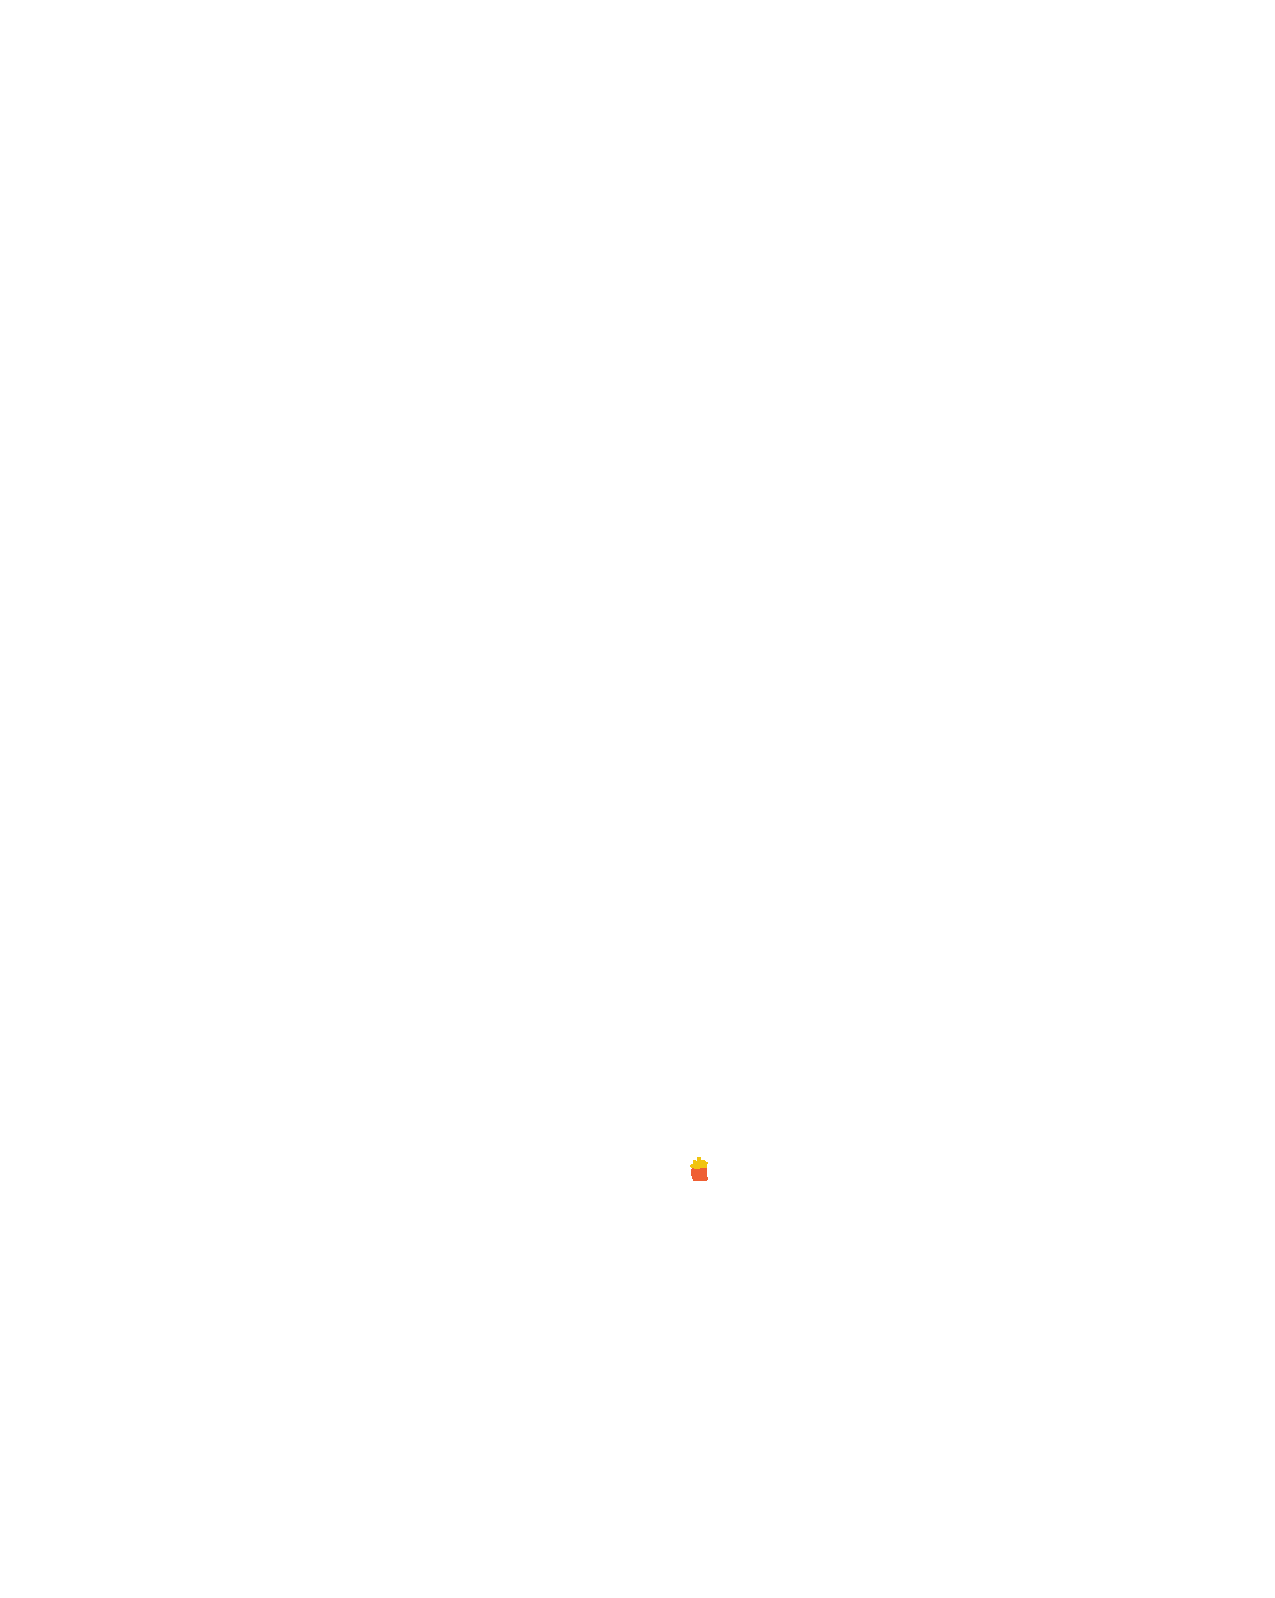
\includegraphics[width=1.5em]{figures/basis_food_icon_fries.pdf}} 
    &
    \eqfig{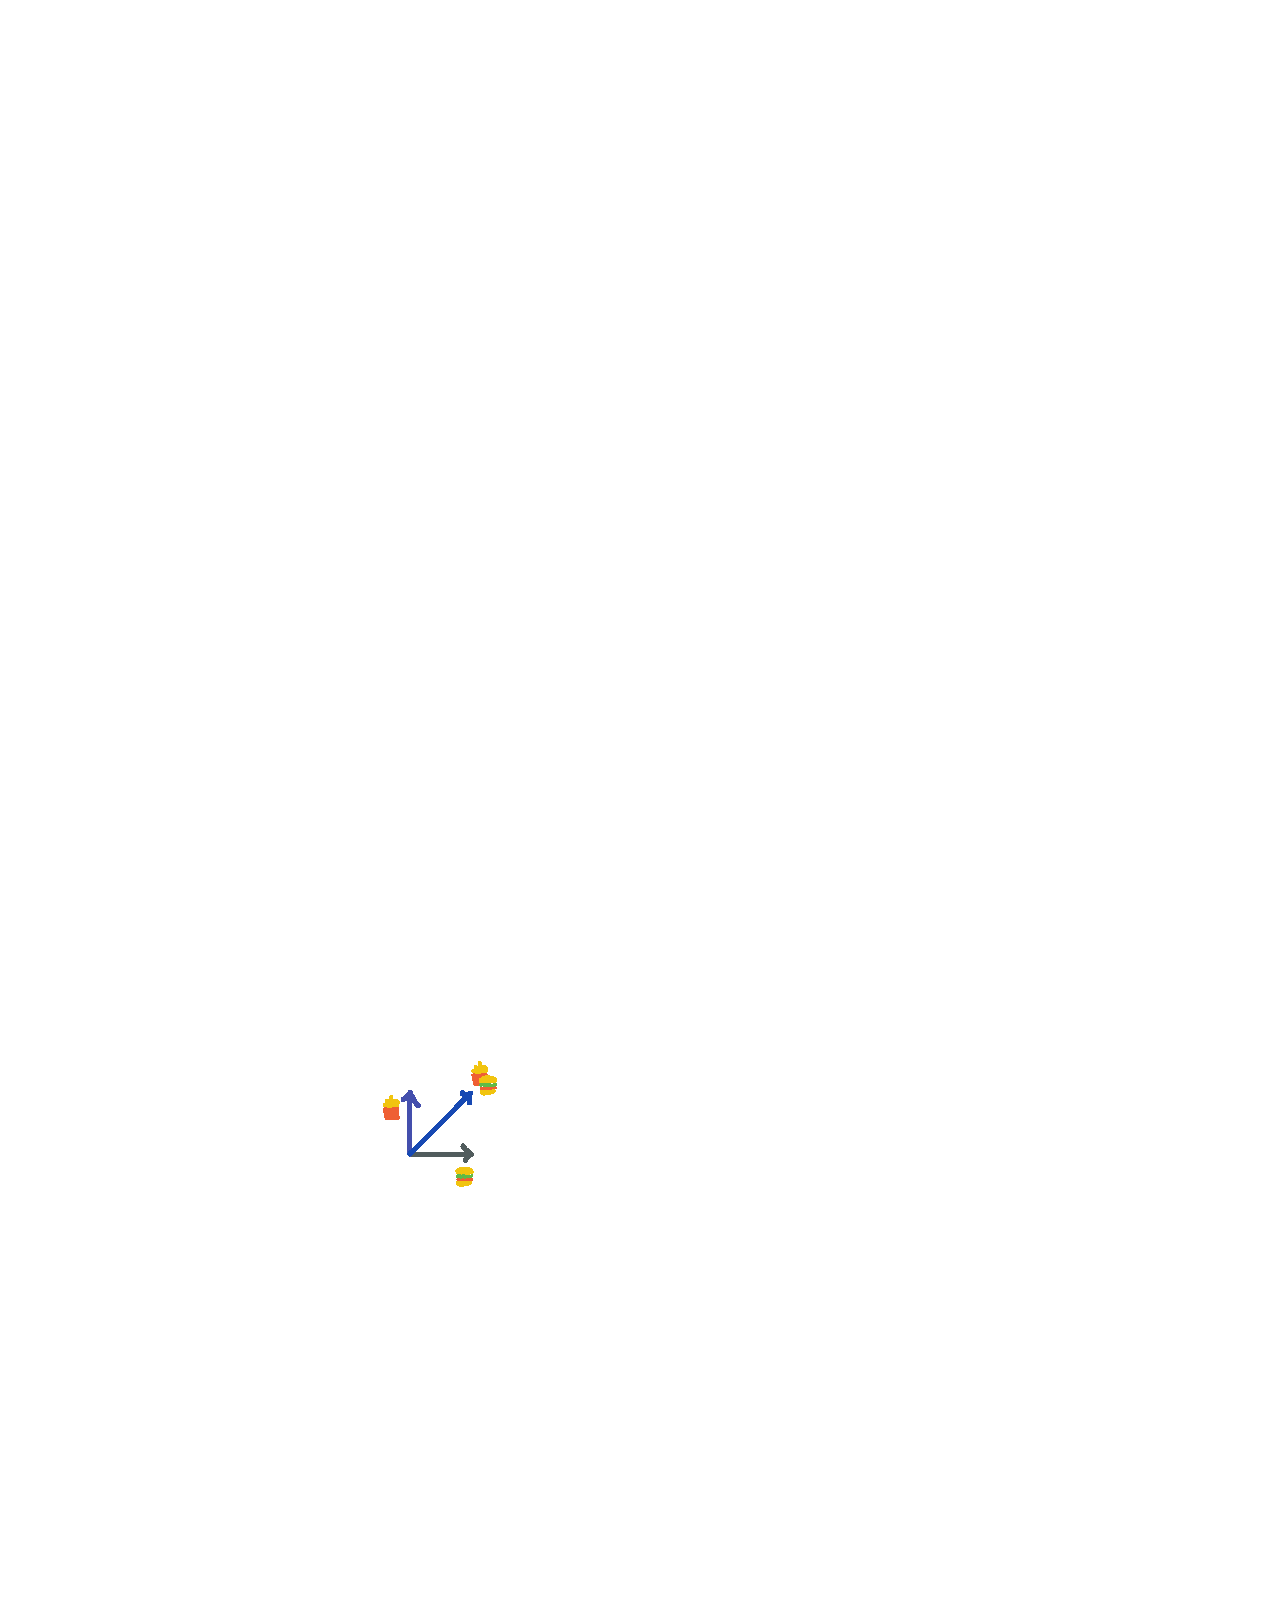
\includegraphics[width=5em]{figures/basis_food.pdf}} 
    \ .
\end{align}
Now an order $\vec{v}$ of two burgers and 1 fries is
\begin{align} 
    \vec{v} &=
    2\bas{f}_1 - \bas{f}_2 = 
    2\eqfig{
\includegraphics[width=1.5em]{figures/basis_food_icon_meal.pdf}}
    -
    \eqfig{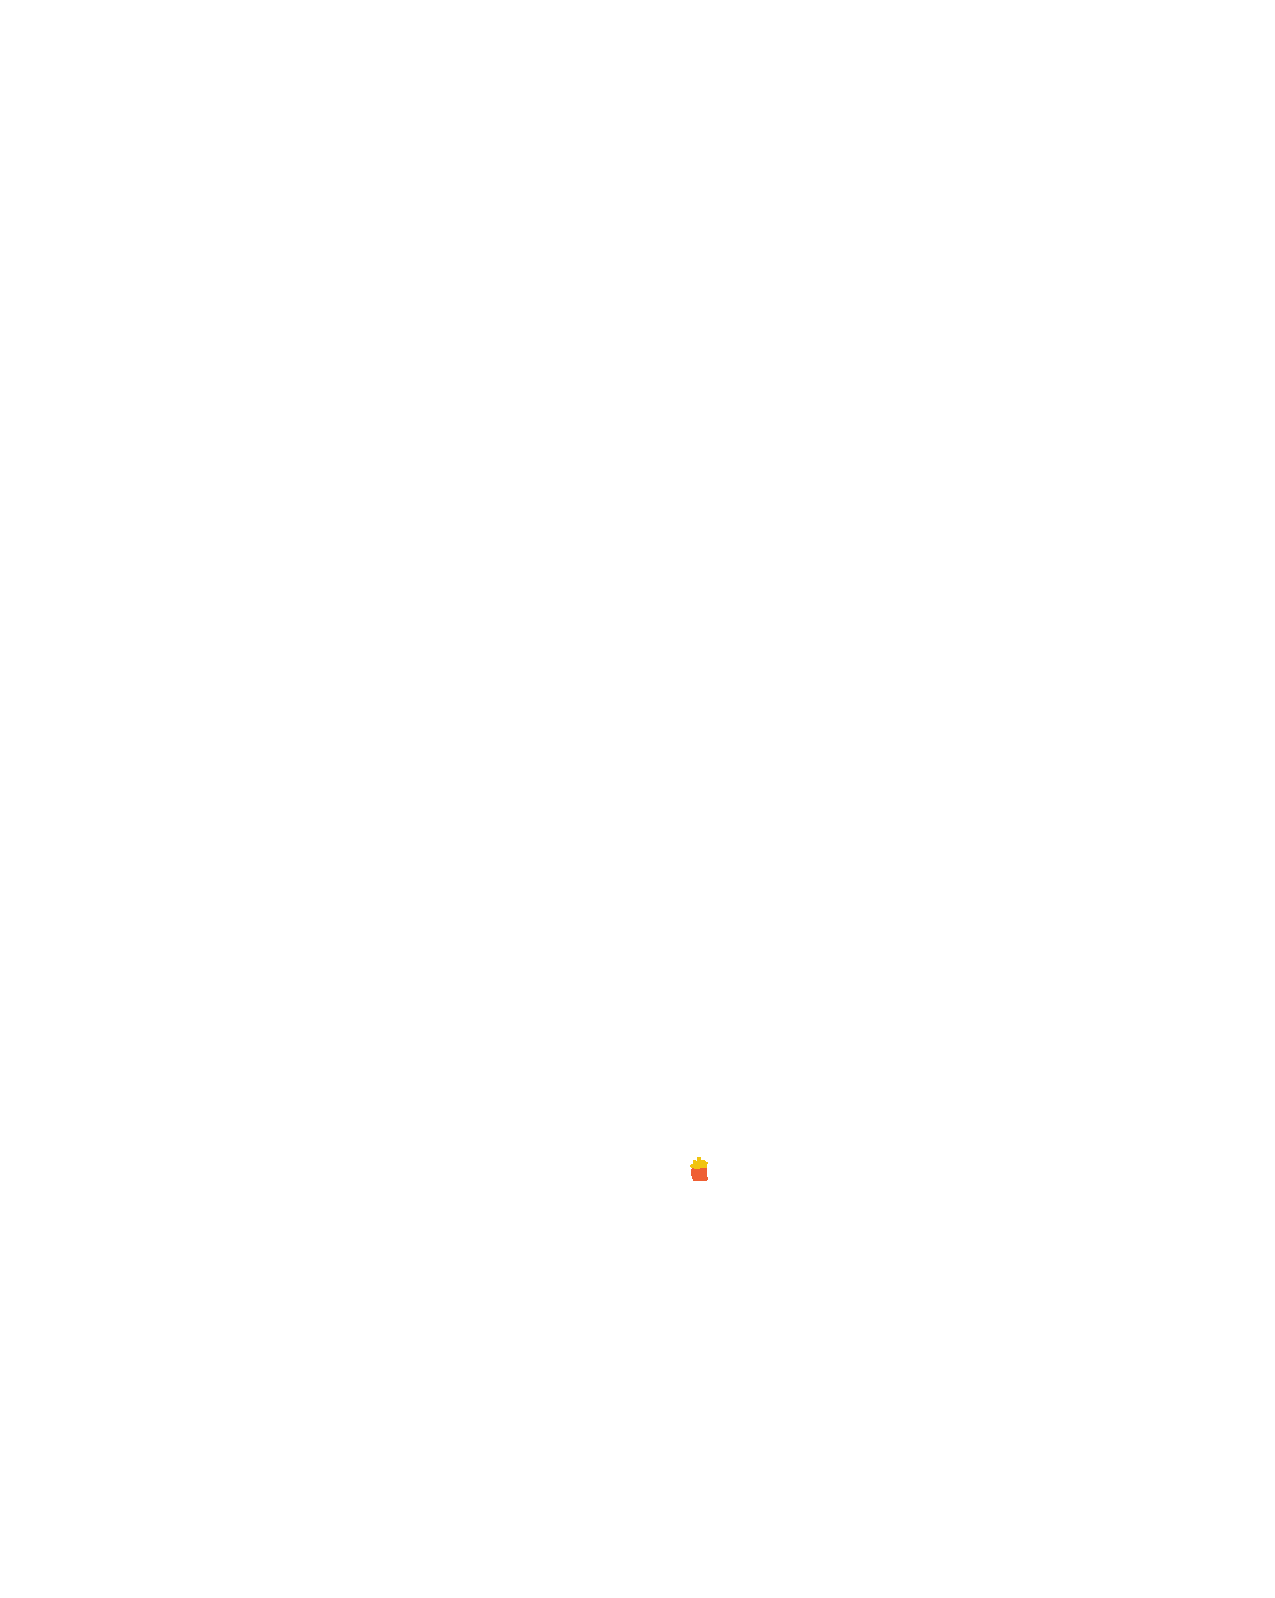
\includegraphics[width=1.5em]{figures/basis_food_icon_fries.pdf}} \ .
    \label{eq:basis:eg:meal:2}
\end{align}
We could also draw these as arrows. It would look something like this:
\begin{center}
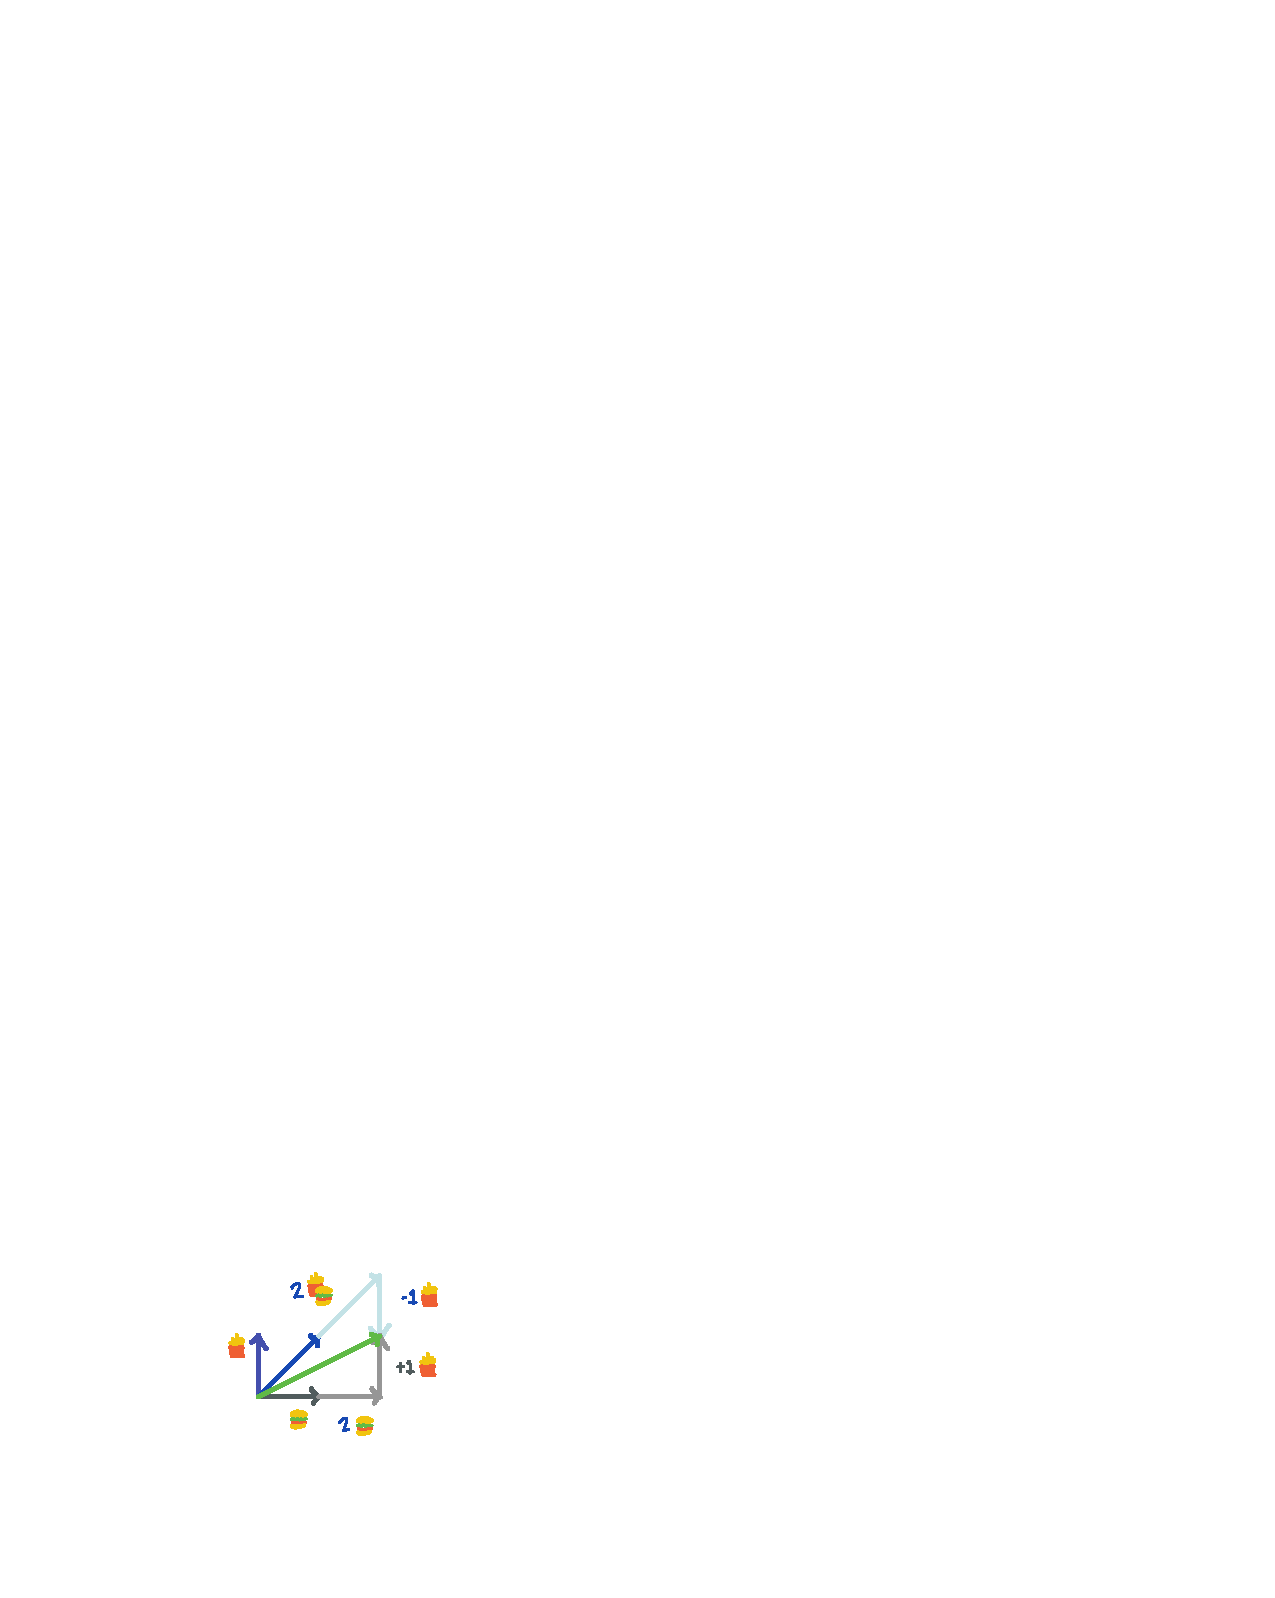
\includegraphics[width=.3\textwidth]{figures/basis_food_eg.pdf}
\end{center}
At this point, you could ask what a \emph{negative} order of fries ($-\bas{f}_2$) means. \emph{I don't know!} Maybe it means I should make fries for the cook? Maybe it means that fast food orders are not described well by vector spaces since the additive inverse may not have a clear meaning. But we have at least we are not talking about columns of numbers.
\end{example}


To make this concrete, please go through Exercise~\ref{ex:fibonacci:space} to meet a somewhat unusual vector space.
\begin{exercise}[Fibonacci sequence space]\label{ex:fibonacci:space}
One of my favorite examples of a vector space is the space of Fibonacci sequences. Fibonacci sequences are infinite lists of numbers $a_i$ that satisfy $a_{i+2} = a_i+a_{i+1}$. Once you specify the first two numbers $a_0$ and $a_1$, you can iteratively generate every other number in the sequence. Each sequence is a vector in the space of possible Fibonacci sequences. Show that this is true by confirming that a linear combination of Fibonacci sequences with each $i^\text{th}$ term added, e.g.\ $(a+b)^i = a_i+b_i$ is also a Fibonacci sequence. Give an example of a basis for the Fibonacci sequences. What is the dimension of the Fibonacci sequence space? \emph{Answer}: the dimension is two, even though each element is an infinitely long list of numbers.
\end{exercise}
\begin{marginfigure}%[th]
    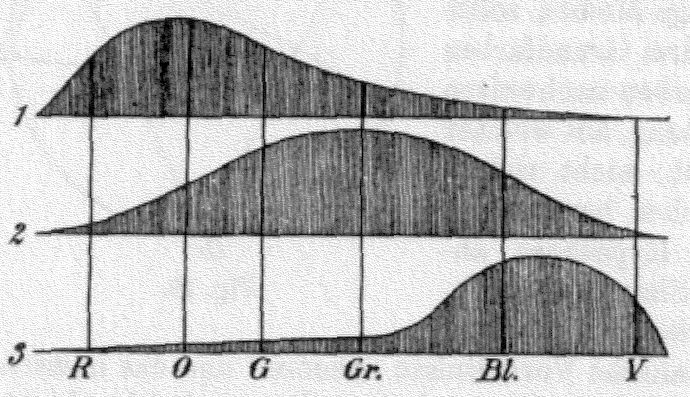
\includegraphics[width=\textwidth]{figures/YoungHelm.jpg}
    \captionsetup{font={scriptsize,sf}}
    \caption{Sketch of Young and Hemholtz (yes, the physicists) spectral sensitivities for different photoreceptors in their trichromatic color space theory. Image from Wikipedia, `Young-Hemholtz theory.'}
    \label{fig:young:hemholtz}
\end{marginfigure}
\begin{example}[Color space]\label{eg:color:space} is a vector space that highlights this idea of a more abstract basis vector. In color theory, all colors are linear combinations of red, green, and blue. This should sound really weird because in physics these colors are simply wavelengths of light: what is special about them? Nothing in nature. What is special is that our eyes have three types of color receptor cells, see Figure~\ref{fig:young:hemholtz}.\footnote{Animals can have different number of color receptor cells. One great place to read about this is Ed Yong's book, \emph{An Immense World}. Color space for those animals has a different dimension than ours.} Each type is sensitive to a certain window of the visible spectrum. We call these human eye responses the colors red, green, and blue. When we add colors, what we really mean is we're adding ``responses'' to a particular spectrum of light. When we add colors, we are not adding electromagnetic waves: we are adding neurological responses. For each type of color-sensitive cell, one `blip' of neural response is a basis vector for our color response. The sensation of a particular color is a linear combination of this basis. An actual human being is not sensitive to the whole vector space: for example, we cannot add negative colors to our sensory response. This is a fascinating subject and a surprising application of linear algebra.\footnote{There are some great YouTube videos on this. Here are a few: \url{https://www.youtube.com/watch?v=xAoljeRJ3lU}, \url{https://www.youtube.com/watch?v=AS1OHMW873s}, \url{https://www.youtube.com/watch?v=99v96TL-tuY}.} The sense in which a color is an overlap integral of a cell's sensitivity to different frequencies of light times the distribution of photons over frequency happens to also be a precursor to the inner product on infinite dimensional spaces.
\end{example}



\subsection{Changing basis} 
\label{sec:sub:basis:changing}

We started this section off by saying that the two of us just agreed on some set of basis vectors. Maybe we do not agree on a set of basis vectors. Maybe I am a little weird and I choose a set of basis vectors that seem very strange to you; this very strange basis does \emph{not} have to be aligned in any particular way.\sidenote{If you are about to say the word \emph{orthonormal}, then stop right there. We do not yet have the mathematical machinery to define orthogonality or normality.} 

\paragraph{A very silly basis}
Here is my silly choice of basis. To help us be very careful, I use square brackets for the components that \emph{you} would measure using \emph{your} basis. 
\begin{align}
    \bas{f}_1 &=
    \begin{bmatrix}
        3 \\ 1
    \end{bmatrix}
    &
    \bas{f}_2 &=
    \begin{bmatrix}
        2 \\ 2
    \end{bmatrix} \ .
\end{align}
All of my vectors are defined with respect to my basis. In fact, all the above line means is
\begin{align}
    \bas{f}_1 &= 3\bas{e}_1 + \bas{e}_2
    &
    \bas{f}_2 &= 2\bas{e}_2 + 2\bas{e}_2
    \ .
    \label{eq:change:basis:eg:1}
\end{align}
We can write this even more succinctly using tensors:
\begin{align}
    \bas{f}_i &= \bas{e}_j T\aij{j}{i} \ .
    \label{eq:change:basis:eg:2}
\end{align}
\begin{exercise}
What are the components of $T\aij{j}{i}$? \textsc{Partial answer:} $T\aij{1}{2} = 2$.
\end{exercise}


I can define a vector $\vec{a}$ with components $\alpha^{1,2}$ and package the components into a column with round brackets:
\begin{align}
    \vec{a} 
    = \begin{pmatrix}
        \alpha^1 \\ \alpha^2
    \end{pmatrix}
    =
    \alpha^i \bas{f}_i  \ .
\end{align}
What does this mean \emph{to you?} To figure this out, you would just insert the conversion \eqref{eq:change:basis:eg:1}:
\begin{align}
    \vec{a} = \alpha^i \bas{f}_i = \alpha^i T\aij{j}{i} \bas{e}_j = (\alpha^i T\aij{j}{i})\bas{e}_j \equiv \beta^j \bas{e}_j \ .
\end{align}
From this we find that the components of the vector $\vec{a}$ in your $\bas{e}_i$ basis are
\begin{align}
    \beta^j = \alpha^i T\aij{j}{i} \ . 
    \label{eq:beta:alpha:T:convert}
\end{align}
\begin{exercise}
Explicitly write out the $\beta^j$. \textsc{Partial answer:} $\beta^1 = 3\alpha^1 + 2\alpha^2$.
\end{exercise}


If I told you that I have a vector whose components---in my $\bas{f}$ basis---are
\begin{align}
    \alpha^1 &= 2 & \alpha^2 &= 3    
\end{align}
the you would understand that
\begin{align}
    \vec{a} 
    = \begin{pmatrix}
        \alpha^1 \\ \alpha^2
    \end{pmatrix}
    =
        \alpha^i \bas{f}_i 
        =
        2
    \begin{bmatrix}
        3 \\ 1
    \end{bmatrix}
    +
    3
    \begin{bmatrix}
        2 \\ 2
    \end{bmatrix}
    =
    \begin{bmatrix}
        12 \\
        8
    \end{bmatrix} 
    \equiv
    \begin{bmatrix}
        \beta^1 \\
        \beta^2
    \end{bmatrix}
    \ .
\end{align}
\begin{exercise}
Verify that these values of $\alpha^i$ and $\beta^i$ satisfy \eqref{eq:beta:alpha:T:convert}.
\end{exercise}
I am being \emph{very} careful here to distinguish between round and square brackets.
In tern, we must be \emph{very} careful in how we interpret this! The round brackets and the square brackets\sidenote{I just made up this notation for illustrative purposes.} are totally different objects. So the following statement is true:
\begin{align}
    \vec{a} = \begin{pmatrix}
        2 \\ 3
    \end{pmatrix}
    = 
    \begin{bmatrix}
        12 \\ 8
    \end{bmatrix} \ .
\end{align}
There is no paradox here: the column in round brackets are the components in the $\bas{f}$ basis while the column in square brackets are the components in the $\bas{e}$ basis. 


\paragraph{General discussion} The square and round bracket notation is somewhat cumbersome and non-standard. Instead, let us propose a notation that is just as cumbersome but more transparent:
\begin{align}
    \begin{pmatrix}
        \alpha^1\\
        \alpha^2\\
        \vdots
    \end{pmatrix}_{\bas{f}}
    &= \alpha^i \bas{f}_i
    &
    \begin{pmatrix}
        \beta^1\\
        \beta^2\\
        \vdots
    \end{pmatrix}_{\bas{e}}
    &= \beta^i \bas{e}_i \ .
\end{align}
A key idea is to see how we convert between bases.\sidenote{The plural of basis is \emph{bases} and is pronounced `bay-sees.' As a linguistic excursion, you can look up the plural of `hippopotamus.'}
\begin{align}
    \bas{f}_i = T\aij{j}{i} \bas{e}_j \ .
    \label{eq:change:of:basis:matrix:1}
\end{align}
We see that in the $\bas{e}$ basis,
\begin{align}
    \bas{f}_1 &=
    \begin{pmatrix}
        T\aij{1}{1}
        \\
        T\aij{2}{1}
        \\
        \vdots
    \end{pmatrix}_{\bas{e}}
\end{align}
and more generally,
\begin{align}
    \bas{f}_i &=
    \begin{pmatrix}
        T\aij{1}{i}
        \\
        T\aij{2}{i}
        \\
        \vdots
    \end{pmatrix}_{\bas{e}} \ .
\end{align}
And so we find the following rule.
\begin{newrule}[Change of basis matrix]\label{rule:change:of:basis:matrix}
Let $T\aij{i}{j}$ be the change of basis matrix defined by \eqref{eq:change:of:basis:matrix:1}. Then  the \emph{columns} of the matrix representation of $T\aij{i}{j}$ with the components of the $\bas{f}$ basis vectors written in the $\bas{e}$ basis:
\begin{align}
    \begin{pmatrix}
        T\aij{1}{1} & T\aij{1}{2} & \cdots \\
        T\aij{2}{1} & T\aij{2}{2} & \cdots \\
        \vdots & \vdots &\ddots  
    \end{pmatrix}
    &
    =
    \begin{pmatrix}
        | & | & \cdots \\
        \bas{f}_1 & \bas{f}_2 & \cdots \\
        | & | & \ddots 
    \end{pmatrix} \ .
\end{align}
\end{newrule}
Now let me take a moment to throw up swaths of caution tape here. The reason why the components of $\bas{f}_i$ in the $\bas{e}$ basis are given by the \emph{columns} of $T\aij{i}{j}$ has to do with our choice of how $T\aij{i}{j}$ is defined in \eqref{eq:change:of:basis:matrix:1}. In our strict index convention, \eqref{eq:change:of:basis:matrix:1} is the \emph{only} structure that makes sense.\sidenote{You could have defined a tensor $S_i^{\phantom{i}j}$ such that $\bas{f}_i = S_i^{\phantom{i}j} \bas{e}_j$, but we can equivalently define a matrix $T\aij{j}{i} = S_i^{\phantom{i}j}$ that does the same thing. If you are thinking about saying $S$ and $T$ transposes of each other---hold your horses! We do not yet have the machinery to define this.} 

We could then ask a separate question: if we know the components of a vector in the $\bas{e}$ basis, $\beta^i$, what are the components in the $\bas{f}$ basis? Then we can take \eqref{eq:change:of:basis:matrix:1} and act on both sides with the inverse transformation $(T\inv)\aij{i}{k}$
\begin{align}
    (T\inv)\aij{i}{k}T\aij{j}{i}\bas{e}_j &= (T\inv)\aij{i}{k}\bas{f}_i \\
    \delta^j_k \bas{e}_j &= (T\inv)\aij{i}{k}\bas{f}_i\\
    \bas{e}_k &=(T\inv)\aij{i}{k}\bas{f}_i \ ,
    \label{eq:intermediate:e:Tinv:f}
\end{align}
Where we use the Kronecker-$\delta$ from \eqref{eq:kronecker:delta}.
% 
Contracting both sides \eqref{eq:intermediate:e:Tinv:f} by the $\bas{e}$ basis components $\beta^k$ then gives an expression for the $\alpha^k$ components in the $\bas{f}$ basis:
\begin{align}
   \beta^k \bas{e}_k &=(T\inv)\aij{i}{k} \beta^k \bas{f}_i \equiv \alpha^i \bas{f}_i \ .
\end{align}
In other words,
\begin{align}
    \alpha^i = (T\inv)\aij{i}{k} \beta^k \ .
\end{align}
Of course, at this point you can wonder about what to do if $T$ is \emph{not} an invertible matrix---and under what conditions would that be the case? Evidently we should put some thought into what a `good' basis might be, and part of that definition is likely to involve the invertibility of the transformation between different `good' bases.

\begin{bigidea}\label{idea:2d:chart}
In physics, a choice of basis often corresponds to a reference frame. For example, we could imagine trying to look at a paper map\footnote{In ancient times maps used to be printed on large pieces of paper that were folded up. Ancient navigators would find shared community in trying to re-fold these maps so that they might fit back into their glove compartments.} while standing in Parking Lot 13 at \acro{UC R}iverside. There is a two dimensional vector space of directions from where we are standing. A natural basis is 
\begin{align}
    \bas{e}_1 &= \text{step forward}\\
    \bas{e}_2 &= \text{step to the right} \ .
\end{align}
Taking a two steps to the left would be $-2\bas{e}_2$. Then I could use my map and tell you that the Physics department is located\footnote{Nevermind that `position vectors' are not a sensible thing. As an exercise, you can try to rephrase this example in terms of velocities. It gets clunky: you are trying to throw a football with some velocity so that it reaches the physics department in a certain fixed amount of time. Analogies are like undergrads... \url{https://phdcomics.com/comics/archive.php?comicid=439}} at $900\bas{e}_1$. This is only correct if my $\bas{e}_1$ basis vector is pointing east; that is, if I am facing east. If you happen to be facing north-east, then your basis vectors would be oriented differently. Perhaps $\bas{f}_1$ still means a `step forward,' but now it is a step in the north-east direction.

We want to be able to describe physical situations in different orientations. It is often easier to describe a problem in a different frame. For example, the frame where the angular momentum (pseudo-)vector is pointed in the $z$ direction, or where the moment of inertia tensor is diagonal. In relativity, it is usually helpful to be able to boost to the rest frame of a moving body.

A more sophisticated version of a change of basis is the description of a quantum particle using its position versus its momentum. Some problems are much easier to solve if you describe the particle in terms of its momentum, while others are easier if you use position. One of the curiosities of quantum mechanics is that these two descriptions turn out to be incompatible, as manifested in the Heisenberg uncertainty relations.

All this is to say that yes: changing basis is a big $\bas{f}$'ing deal.\footnote{To paraphrase a former vice president.}
\end{bigidea}



\subsection{Goldilocks dimension} % Why isn't the modern telling called ``Karen and the three bears?''

Recall from \eqref{eq:linear:combination:looks:like:basis} that the span of a set of vectors $\vec{v}_1, \cdots, \vec{v}_N$ is the vector space $V$ of all linear combinations of those vectors. This makes us want to identify those vectors as a basis for $V$. \emph{Not so fast}. For any vector space $V$, there is a `correct' number of basis vectors vectors called the \textbf{dimension}\index{dimension} of $V$, or $\text{dim}\,V$. This dimension is the minimum number of good basis vectors that you need to describe any vector in $V$. To write it technically, $\text{dim}\,V$ is the smallest counting number $d$ such that
\begin{align}
    \forall \vec{v} \in V :\; \vec{v} = v^1 \bas{e}_1 + \cdots + v^{d}\bas{e}_{d} \ .
\end{align}
The symbol $\forall$ means ``for all,'' so the above line says: for all (really: for \emph{any}) vector $\vec{v}$ in the vector space, $\vec{v}$ is a linear combination of $d$ basis vectors. The dimension of $V$ is the smallest number $d$ for which this is true. 

If your number of proposed basis vectors is larger than this dimension then vectors do not have a unique expansion. If your number of proposed basis vectors is smaller than this dimension, then there are vectors in $V$ that \emph{cannot} be described by linear combinations of your basis vectors. And even if your number of proposed basis vectors is \emph{just right} and exactly equal to $\text{dim}\,V$, you could \emph{still} fail because some of your basis vectors are actually combinations of other basis vectors. Let us go through these cases sequentially.

\subsubsection{Too many basis vectors}

Start with the following example:
\begin{example}
Suppose you have the following proposed basis:
\begin{align}
    \bas{e}_1 &=
    \begin{pmatrix}
        1\\
        1
    \end{pmatrix}
    &
    \bas{e}_2 &=
    \begin{pmatrix}
        2\\
        1
    \end{pmatrix}
    &
    \bas{e}_3 &=
    \begin{pmatrix}
        -1\\
        \pp 1
    \end{pmatrix} \ .
    \label{eq:eg:too:many:basis:vectors:basis}
\end{align}
Suppose I then give you the vector
\begin{align}
    \vec{v} &=
    \begin{pmatrix}
        3 \\ 1
    \end{pmatrix} \ .
\end{align}
What is the linear combination of your basis vectors that produces $\vec{v}$? In other words, what are the $v^i$ so that
\begin{align}
    \vec{v}= v^i \bas{e}_i \, ?
\end{align}
You can write this as a system of equations. One solution is
\begin{align}
    \vec{v} &= -1\bas{e}_1 + 3\bas{e}_2 + 0\,\bas{e}_3 
    &
    \begin{pmatrix}
        v^1 \\ v^2 \\ v^3
    \end{pmatrix}
    =
    \begin{pmatrix}
        -1 \\ \pp 3 \\ \pp 0
    \end{pmatrix} \ .
\end{align}
Great, problem solved, right? Not quite. We could have \emph{alternatively} written
\begin{align}
    \vec{v} &= 0\,\bas{e}_1 + \frac{4}{3}\bas{e}_2 - \frac{1}{3}\bas{e}_3 
    &
    \begin{pmatrix}
        v^1 \\ v^2 \\ v^3
    \end{pmatrix}
    =
    \begin{pmatrix}
        \pp 0 \\ \pp 4/3 \\ - 1/3
    \end{pmatrix} \ .
\end{align}
Now we should be concerned. For the \emph{same} basis, there are at least \emph{two} different sets of coefficients that describe the \emph{same} vector! How are we supposed to keep track of the fact that there are \emph{degeneracies} where different combinations of components $v^i$ actually mean the \emph{same} vector? That would be madness.\sidenotemark
\end{example}\sidenotetext{This is absolutely silly to do, but it turns out there are cases in physics where we make use of this type of madness. These are called \emph{gauge theories}. An example of a gauge theory is electromagnetism, where there is a redundancy that we call a \emph{gauge symmetry}. This corresponds to the fact that many different choices of gauge potential (the electric and vector potentials) produce the same physical electric and magnetic fields. An excellent introduction to this idea is \arXiv{hep-th/0611201}.}
\begin{exercise}
Write out and solve the system of equations from the previous example. Show that there are an infinite number of solutions. In fact, these solutions are a line in a three-dimensional space.
\end{exercise}

Evidently you can have \emph{too many} basis vectors. In the above example, we could have taken any two of the three basis vectors and still described the same vector space. That vector space thus has dimension two. We can see that one manifestation of the fact that we had too many basis vectors that we had more components $v^i$ than the dimension of the space.\sidenote{Indeed, the fact that the basis vectors themselves could be written with only two components with respect to the canonical basis tells us we are doing something silly with \emph{three} basis vectors.}

So if you have too many basis vectors, there is no unique way of assigning vector components $v^i$ to a vector $\vec{v}$. We do not want to have too many basis vectors. 


\subsubsection{Too few basis vectors}

Let us see what happens if we go the other way. 
\begin{example}
Suppose you have the following proposed basis:
\begin{align}
    \bas{e}_1 &=
    \begin{pmatrix}
        1\\
        1\\
        0
    \end{pmatrix}
    &
    \bas{e}_2 &=
    \begin{pmatrix}
        \pp 1\\
        -1\\
        0
    \end{pmatrix}
    \ .
    \label{eq:eg:too:few:basis:vectors:basis}
\end{align}
Suppose I then give you the vector
\begin{align}
    \vec{v} &=
    \begin{pmatrix}
        3 \\ 1 \\ 1
    \end{pmatrix} \ .
\end{align}
What is the linear combination of your basis vectors that produces $\vec{v}$? Once again, we solve the component-wise system of equations 
\begin{align}
    \vec{v}= v^i \bas{e}_i \, ,
\end{align}
where we recognize that there is only a sum over $i=1$ and $i=2$. There is \emph{no} third basis vector. We can uniquely assign coefficients to match the top two components of $\vec{v}$, but there is \emph{no} linear combination of $\bas{e}_1$ and $\bas{e}_2$ that can produce a non-zero element in the last component. Thus $\vec{v}$ is \emph{not} in the span of $\vec{e}_1$ and $\vec{e}_2$. If we want $\vec{v}$ to be part of the vector space $V$, we need to augment our basis with another basis vector.
\end{example} 
\begin{exercise}
Write out and solve the system of equations from the previous example. Show that there are more constraints than free parameters (coefficients $v^i$) and that the constraints cannot be simultaneously. Give an example of a third basis vector that would allow you to uniquely write the vector $\vec{v}$.
\end{exercise}

If you have too few basis vectors, then there seems to be more `space' than the vector space spanned by your basis. That is fine, you just have to be aware that \emph{too few basis vectors} means that this reduced set of basis vectors spans what is called a \textbf{subspace}\index{subspace}. This is the set of vectors spanned by an `incomplete' basis.\sidenote{This is all somewhat hand-wavey because as we abstract away the meaning of the basis vectors it is not always obvious when there is more `space' to be described. In Example~\ref{eg:color:space}, you could say that color space is three dimensional. Or you could say that this is a subspace of a larger color space where we imagine that humans had a fourth type of cone cell. Mantis shrimps have a 16-dimensional color space.}



\subsubsection{Just the right number of basis vectors}

Suppose you have just the right number of basis vectors. You should be all good, right? Maybe not. 
\begin{example}
The canonical basis \eqref{eq:canonical:basis} is an example of a good basis. Let us consider the case of a three-dimensional vector space spanned by the first three of these basis vectors, $\bas{e}_{1,2,3}$. Now consider the following basis:
\begin{align}
    \bas{f}_1 &=
    \begin{pmatrix}
    1 \\ 1 \\ 2  
    \end{pmatrix}_{\bas{e}}
    &
    \bas{f}_1 &=
    \begin{pmatrix}
    1 \\ 0 \\ 1  
    \end{pmatrix}_{\bas{e}}
    &
    \bas{f}_1 &=
    \begin{pmatrix}
    0 \\ 1 \\ 1  
    \end{pmatrix}_{\bas{e}} \ .
    \label{eq:eg:basis:lin:dependent}
\end{align}
Remember that the subscript $\bas{e}$ reminds us that those columns are written in the canonical basis.
You know the name of the game. If we have a vector $\vec{v}$, can you solve for the coefficients $v^i$ in the $\bas{f}$ basis:
\begin{align}
    \vec{v} = 
    \begin{pmatrix}
        2 \\ 2 \\ 3
    \end{pmatrix}
    = v^i \bas{f}_i \, ?
\end{align}
What are the coefficients/components $v^i$? It turns out that there is no solution.
\end{example}
\begin{exercise}
Write out the system of three equations for the three components $v^i$ and show that they are \emph{degenerate} and that for a general vector $\vec{v}$ in the $\bas{e}$ basis one \emph{cannot} find solutions for $v^i$. Give an example of a vector that \emph{can} be written in the $\bas{f}$ basis. Argue that vectors that can be written in the $\bas{f}$ basis form a \emph{two} dimensional subspace.
\end{exercise}

Can you see what went wrong in the $\bas{f}$ basis in the previous example? One hint is that
\begin{align}
    \bas{f}_3 = \bas{f}_2 - \bas{f}_1 \ .
\end{align}
% {eq:eg:basis:lin:dependent}
In other words: one of the basis vectors is a \emph{linear combination} of the others.\sidenote{It does not matter which one. In this example, you could pick any basis vector and write it in terms of the other two.} We say that this set of vectors is \textbf{linearly depenent}\index{linearly dependent}.  Because you can replace $\bas{f}_3$ with a linear combination, then any proposed linear combination $v^i$ of the three $\bas{f}$ basis vectors can be more simply written as a linear combination of only two basis vectors:
\begin{align}
    v^i \bas{f}_i = (v^1-v^3)\bas{f}_1 + (v^2+v^3)\bas{f}_2 \equiv w^1 \bas{f}_1 + w^2\bas{f}_2 \ .
\end{align}
On the right-hand side we show that could have otherwise written any such ``three component'' vector $v^i$ as a linear combination of two basis vectors. This means that vectors $v^i\bas{f}_i$ are actually part of a two-dimensional subspace and should properly be described by only two basis vectors. If we want to describe the entire three-dimensional space spanned by $\bas{e}_{1,2,3}$, we need a third \emph{linearly independent} basis vector. 

The example is in contrast to, say, the canonical basis, which is \textbf{linearly independent}\index{linearly independent}. There means that there no vector $\bas{e}_i$ that can be written as a linear combination
\begin{align}
    \bas{e}_1 \neq \sum_{j \neq 1} \alpha^j \bas{e}_j \ .
\end{align}
This is obvious in the canonical basis because each basis vector is only non-zero for a unique index $i$.


\begin{bigidea}[Basis]
When we say that we have a basis $\bas{f}$ for a vector space $V$, we mean that
\begin{enumerate}
    \item $\text{Span}(\bas{f}_1, \cdots \bas{f}_N) = V$. This means that any vector in $V$ can be written $\vec{v} = v^i \bas{f}_i$. If you cannot do this, then you do not have enough [independent] basis vectors.
    \item The basis vectors $\bas{f}_{1,\cdots,N}$ are each linearly independent from one another. This means that there is no basis vector that can be written as a linear combination of the other basis vectors. If this is not true, then you have too many basis vectors: at least one is linearly dependent on the others.
\end{enumerate}
These conditions are assumed when we say we have a basis. We have not said anything about what makes a \emph{good} basis, though it is clear that the canonical basis \eqref{eq:canonical:basis} is a good basis.
\end{bigidea}
You may have a sense in which basis vectors should be orthonormal. We still do not yet have the machinery to define orthonormality.s



\section{Linearity}

\begin{bigidea}[Linearity] We say that a function $f$ is \textbf{linear}\index{linear} if linear combinations of arguments (inputs) produce linear combinations of outputs. Suppose $f$ is a function that takes in some object, $\vec{x}$. The output of $f$ can be the same type of object or a different type of object. Then $f$ is linear if for any two input-type objects $\vec{x}$ and $\vec{y}$ and any two numbers $\alpha$ and $\beta$:
\begin{align}
    f(\alpha\vec{x}+ \beta\vec{y}) = \alpha f(\vec{x}) + \beta f(\vec{y}) \ .
    \label{eq:linear:function}
\end{align}
Let us suppose the inputs $\vec{x}$ and $\vec{y}$ are vectors. Then the argument on the left-hand side is a linear combination of vectors, which is itself a vector. Linearity means that if we already know what $f(\vec{x})$ and $f(\vec{y})$ are, then we do not have to recalculate anything to find $f(\alpha\vec{x}+\beta\vec{y})$; we simply take a linear combination of the outputs with the same coefficients, $\alpha$ and $\beta$.
\end{bigidea}

\begin{example}
Consider functions from $\mathbbm{R}\to\mathbbm{R}$. These are ordinary functions that take numbers and return numbers. Using our definition, $f(x) = ax$ is linear because
\begin{align}
    f(\alpha x+\beta y) = a(\alpha x + \beta y)  = a\alpha x + a \beta y =\alpha f(x) + \beta f(y) \ .
\end{align}
\end{example}

\begin{exercise}
Show that the equation for a line $f(x) = ax + b$ is \emph{not linear} for $b\neq 0$.\sidenotemark

Deduce that it is generally true that a linear function must satisfy $f(\vec{0}) = 0$. \textsc{Hint}: consider taking linear combinations with $\vec{0}$.
\end{exercise}\sidenotetext{Yes, you heard this correctly. A function that plots to a line in the Cartesian plane is not necessarily \emph{linear}.}

By the way, we often use the term \textbf{map}\index{map} instead of function. I think this is because some people assume that a function only outputs a number, whereas a `map' can take in some object and spit out another object---where the output object may have more structure than a number.\sidenote{For example, it may take in a vector and output a vector.}

\section{Linear Maps}\label{sec:linear:maps}

We may combine the idea of a vector space with our definition of linearity to sharpen some of our language. A \textbf{matrix}\index{matrix} is a linear function that takes vectors and spits out other vectors. We say that these are \emph{linear maps} from $V\to V$. Equivalently, the matrix also takes row vectors and spits out row vectors, so they are also maps from $V^* \to V^*$.  In fact, they are \emph{also} linear functions that take a vector and a row vector into a number:
\begin{align}
    M:\; V\otimes V^* \to \# \ . \label{eq:M:tensor:product}
\end{align}
The left-hand side just says ``$M$ is a map that takes...''
We have introduced the $\otimes$ \textbf{tensor product}\index{tensor product} notation.\sidenote{I'll be real honest with you: sometimes I just write this as $\times$.} The tensor product is like a `multiplication' of \emph{spaces}. 
% 
The above line simply means a linear map that takes an element of $V$ and an element of $V^*$ to produce a number.\sidenote{The $f:V\to\#$ notation does not necessarily mean that $f$ is linear. But in this course we only deal with linear functions/maps. }

This means you can think of row vectors as linear maps from vectors to numbers. In turn, vectors are linear maps that take row vectors to numbers:
\begin{align}
    \row{w}:&\; V\to \# &
    \vec{v}:&\; V^* \to \# \ .
\end{align}
In should be clear that \emph{both} of these refer to $w_iv^i$. If you know all the components of a row vector $w_i$, then I can give you \emph{any} $\vec{v}$ and you can perform the contraction $w_iv^i$ to produce a number. That means the information that you have (the components $w_i$) can be assembled---using our contraction rule---into a machine that takes any vector and spits out a number.

\begin{exercise}
What are all of the possible ways of treating a $(p,q)$ tensor as a linear function? That is: what are the possible inputs for such an object, and for each object, what is the output? For example, if $q\geq 1$, then I can feed a $(p,q)$ tensor a vector and the output is a $(p,q-1)$ tensor.
\end{exercise}

\section{Interlude: some math-speak}

\paragraph{Jargon: functions, maps, transformations} Let us get some terminology sorted out.\sidenote{This paragraph is to establish the correct mathematical jargon. Usually one can get away with being somewhat sloppy and using these terms interchangeably, but we should be clear about the distinction somewhere in these notes.}
A \textbf{function}\index{function} is a mathematical machine that takes some inputs and produces some output. The inputs can be numbers, vectors, or more sophisticated objects. The outputs may also be numbers, vectors, or more sophisticated objects. The outputs do not have to be the same type of object as the inputs---in general they are not.
% 
A \emph{function} that takes one input and returns one output is called a \textbf{map}\index{map}. 
% 
A \emph{map} that takes one type of object and returns the same type of object is called a \textbf{transformation}\index{transform}. Mathy-folks like to draw diagrams like Fig.~\ref{fig:Linear Transformation}.

\begin{figure}[tb]
\sidecaption[][-2\baselineskip]{%
        Example of a linear transformation. The transformation $M$ (for matrix) takes a vector $\vec{v}$ and turns it into a different vector that we call $\vec{v}'$. This new vector is related to $\vec{v}$ by the matrix $\vec{v'}=M\vec{v}$. \emph{Every} vector is transformed under the map $M$. This is an \emph{active transformation} where all vectors transform, but the basis (${\bas{e}}_i$) stays fixed. \label{fig:Linear Transformation}}
        %
        %% \label command inside the \sidecaption command
    \centering
    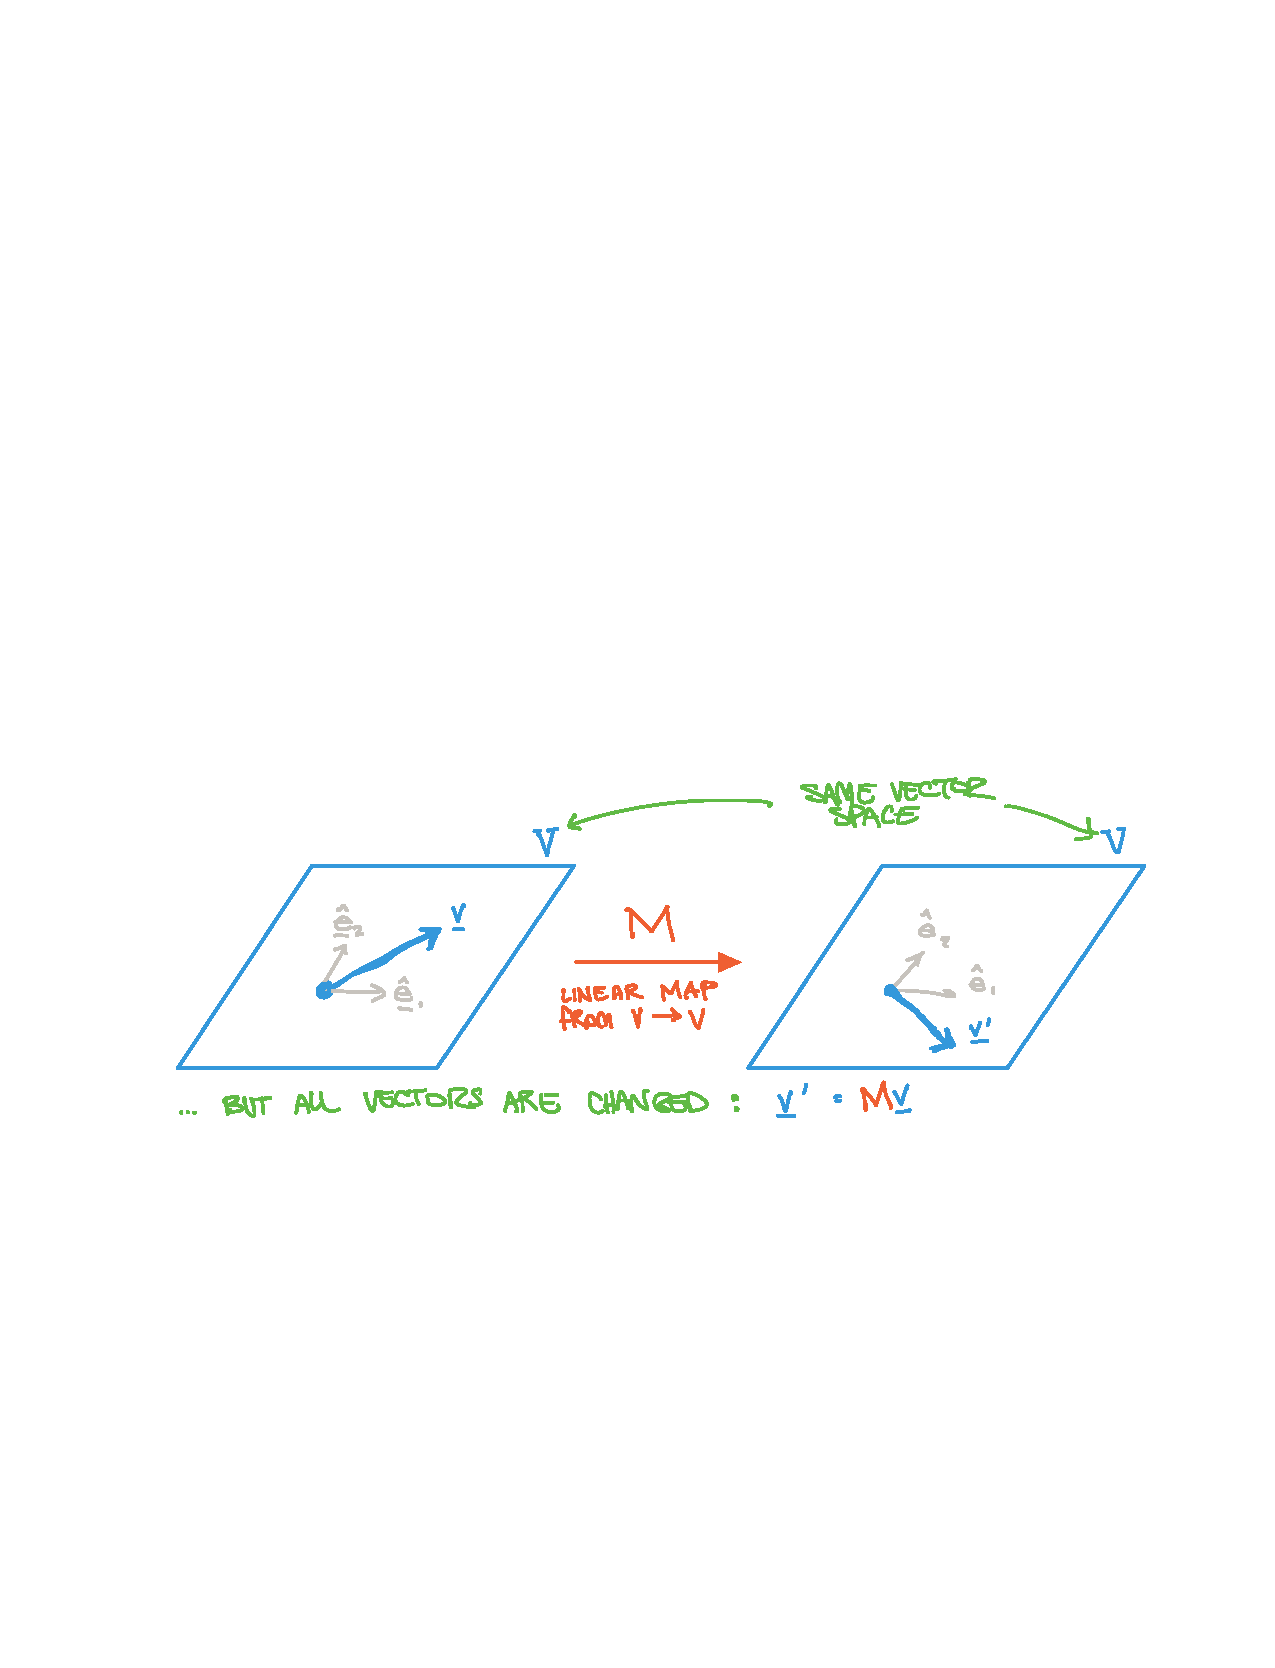
\includegraphics[width=\textwidth]{figures/lineartransformation.pdf}
\end{figure}


\begin{example}
Here are a few examples of each of the above terms:
\begin{itemize}
    \item A price checker at a store takes in barcodes and returns the cost of the item. This is a \emph{map} from barcodes to prices. This is not a map between vector spaces.\sidenotemark
    \item Conversion from kilograms to pounds is a \emph{map} takes a quantity in one unit and converts it to the same quantity in different units. This map is also \emph{linear}: if the input quantity is twice as heavy in kilograms, it will be twice as heavy in pounds. If you add two quantities in kilograms, the mass of the total object in pounds is the sum of the individual masses in pounds.
    \item A function that takes in a vector $\vec{v}\in\mathbbm{R}^2$ and returns $2\vec{v}$ is a transformation. Both the inputs and outputs are vectors in the same vector space. 
\end{itemize}
\end{example}\sidenotetext{At least I cannot figure out a reasonable vector space interpretation. I think I was already pushing it a bit far when we talked about cheeseburger-and-fries space in Example~\ref{ex:cheeseburger:space}.}

\paragraph{More jargon: one-to-one, onto, invertible}

We are going to make a big deal about \textbf{invertible transformations}\index{invertible}. An invertible transformation is one that can be reversed or undone. The transformation need not be linear---though our focus will be linear invertible functions---so for this paragraph let use write $\vec{f}(\vec{v})$ to mean an invertible, not-necessarily-linear transformation. I have even written the function as $\vec{f}$ rather than $f$ to remind us that the output is a vector. Mathematically, an invertible function is one where $\vec{f}^{-1}(\vec{v})$ is defined for any $\vec{v}$ and
\begin{align}
    \vec{f}\inv(\vec{f}(\vec{x})) = \vec{f}(\vec{f}\inv(\vec{x})) = \vec{x} \ .
\end{align}
The \emph{reason} why we care about invertible transformations is precisely the point in \bigidearef~\ref{idea:matrix:inverse:in:physics}: so much of physics is written in the form
\begin{align}
    (\text{operator})\, \ket{\text{state}} = \ket{\text{source}} \ ,
\end{align}
and our job is to invert the operator so that we can figure out what the state is as a function of the source. That is, we are usually given an equation
\begin{align}
    \vec{f}(\vec{x}) = \vec{w} \ ,
\end{align}
and we are given the form of the function $\vec{f}$ and the value of the source $\vec{w}$.\sidenote{Maxwell's equations are like this: on the left-hand side there's some fancy vector calculus differential operator acting on the field that you want to calculate, on the right-hand side there is some kind of charge or current distribution.} Our job is to determine $\vec{x} = \vec{f}\inv(\vec{v})$. 

Sometimes it is the case that $\vec{f}(\vec{x})$ is a pretty nasty function.\sidenote{By nasty I mean nonlinear. By nonlinear I mean \emph{not linear}, where the definition of linearity is \eqref{eq:linear:function}.} So instead of using $\vec{f}$, we can perform a Taylor expansion and consider the \emph{linear} part of $\vec{f}$. From our discussions so far, a linear transformation is represented as a matrix, $M$. Thus we end up writing:
\begin{align}
    \vec{f}(\vec{x}) \approx M\vec{x}  \ ,
\end{align}
and the problem inverting $\vec{f}$ reduces to the problem of inverting a linear transformation $M$. It is for this reason that we make a big deal about understanding when $M$ is invertible and, when it is, how to determine $M\inv$ in a systematic way.\sidenote{In Exercise~\ref{ex:matrix:inversino:the:hard:way} you already showed that finding the inverse of a matrix boils down to writing out and solving a system of equations. This method is intractable for very large matrices. Our goal is to reach infinite-dimensional matrices.}

\begin{example}
A function that takes your student identification number and returns your net\tacro{ID} is one-to-one. Every student identification number corresponds to a unique student with a unique net\tacro{ID}. However, not every net\tacro{ID} belongs to a student---faculty have net\tacro{ID}s but not student identification number, for example---so this function is not invertible. 
\end{example}

A few more bits of jargon. We won't use these, but consider these to be essential tools if you ever find yourself in a verbal sparring match with a mathematician:
\begin{enumerate}
    \item \textbf{Injective}\index{injective}/\textbf{one-to-one}\index{one-to-one}: 
    every output is unique; if you knew the output then you can deduce the input. However there may be some output-class objects that are not the outputs of the function for any input.
    \item \textbf{Surjective}\index{surjective}/\textbf{onto}\index{onto}: every output-class object is the result of some input, however there may be multiple inputs that produce the same output.
    \item \textbf{Bijective}\index{bijective}: this is a fancy name for \emph{invertible}. 
\end{enumerate}
% Every linear function is surjective. 

\begin{example}
Dual vectors are linear functions of vectors to numbers. Any non-zero dual vector $\row{w}$ is surjective. To see this, take any vector $\vec{v}$ and calculate $\row{w}\vec{v}$; call this number $a$. Any other number, say $b$, is the output of $\row{w}$ acting on $(b/a)\vec{v}$. Thus every output-class object (number) is realized as $\row{w}$ acting on some input. 
\end{example}

\begin{example}
In general, dual vectors are \emph{not} injective. For example, consider the dual vector $\row{w}=\begin{pmatrix}
    a & -a
\end{pmatrix}$. Then $\row{w}\vec{v} = 0$ for any vector $\vec{v}$ of the form
\begin{align}
    \vec{v} = 
    \begin{pmatrix}
        b \\ b
    \end{pmatrix}\ .
\end{align}
The zero vector is of this form so that $\row{w}\vec{0}=0$, as required by linearity. 
\end{example}


% Row vectors as 
% The fact that matrices take vectors and return vectors tells us that they enact transformations on the \emph{space} of vectors. Under the action of a matrix, every allowed vector is transformed into a different vector. 


\section{Basis in terms of linear transformations}

\begin{figure}[tb]
    \centering
    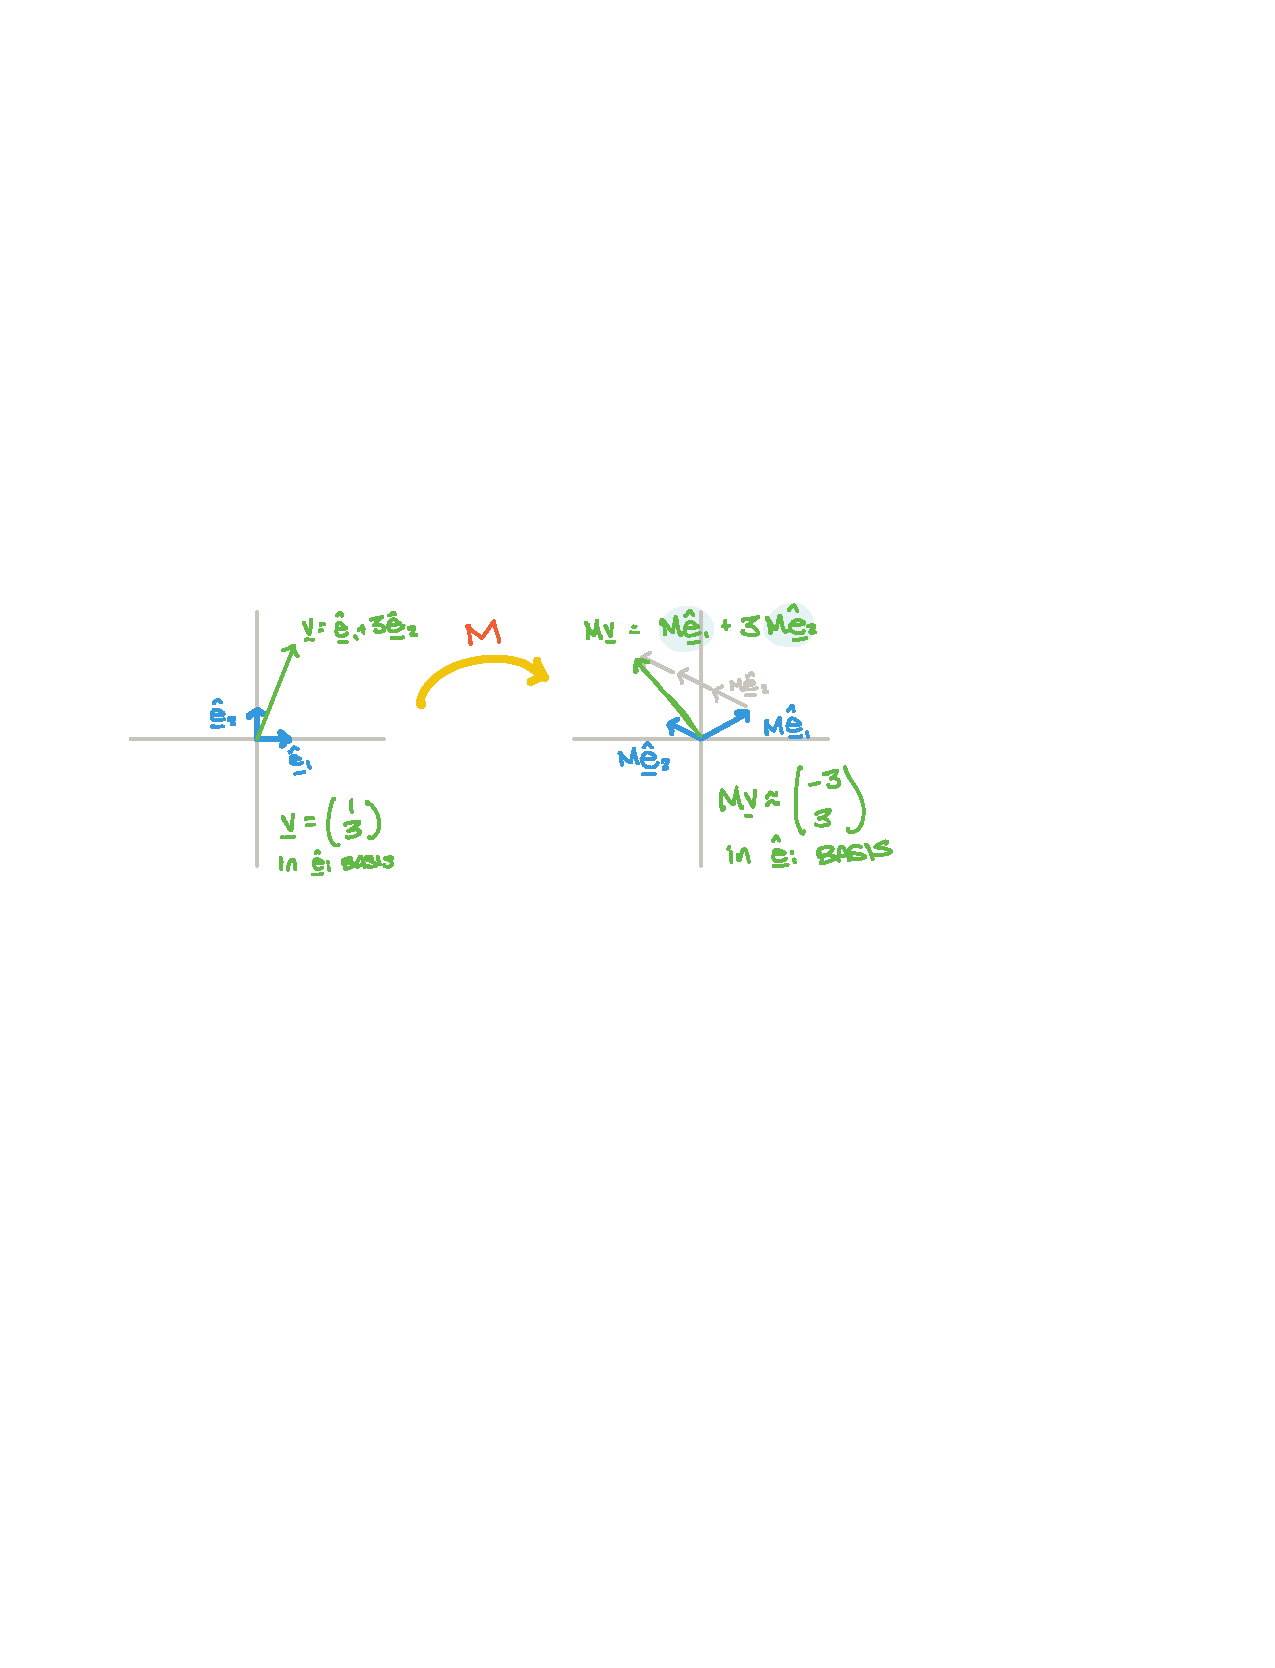
\includegraphics[width=.8\textwidth]{figures/maps_M.pdf}
    \caption{$M$ is a linear transformation from $\RR ^2\to\RR ^2$. If we know the action of $M$ on the basis vectors $\bas{e}_i$ of $\RR ^2$, then we know the action of $M$ on any vector $\vec{v}$.}
    \label{fig:map:M}
\end{figure}

The magic of linearity is that if you know how basis vectors transform, then you know how all vectors transform. This is demonstrated in Figure~\ref{fig:map:M}. In turn, we can understand linear transformations themselves in terms of basis transformations.

\subsection{Basis of row vectors}

We write the basis row vectors as $\rbas{e}^i$ so that any row vector may be written $\row{w} = w_i \rbas{e}^i$. We have again chosen indices so that we may use summation convention. Everything that we have discussed about basis vectors in Section~\ref{sec:basis} carries over, except now the basis vectors are basis \emph{row} vectors. Because row vectors are themselves a vector space, this is not surprising. In fact, this is simply the \emph{duality} between $V$ and $V^*$. 

Now that we are armed with the idea of row vectors\sidenote{a.k.a\ dual vectors, covectors, bras} as linear transformations, we can go further and explain the nature of this duality. Fixing a basis of column vectors in $V$ automatically fixes the basis in $V^*$ in the following way:
% 
\begin{bigidea}[Basis of dual vectors]\label{idea:basis:of:dual:vectors}
Given a basis $\bas{e}_{1,\cdots,N}$ for a vector space $V$, the basis for the vector space $V^*$ is $\rbas{e}^{1,\cdots,N}$ and is defined as follows:
\begin{align}
    \rbas{e}^i\left[ \bas{e}_j \right] = \delta^i_j \ .
    \label{eq:basis:of:dual:vectors}
\end{align}
For example, $\rbas{e}^1\left[\bas{e}_2\right] = 0$ and $\rbas{e}^1\left[\bas{e}_1\right] = 1$.
\end{bigidea}
% 
This merits some reflection. Here is a sequence of thoughts:
\begin{enumerate}
    \item A basis dual vector is an linear map that takes in vectors and returns a number---this is our enlightened definition\sidenote{As opposed to a `sideways vector' or `the same thing as a vector,' which are slightly less enlightened (read: not useful, largely incorrect) definitions.} of a dual vector. 
    \item Because the map is linear, it is sufficient to define its action on a set of basis vectors. 
    \item Given a specific basis $\bas{e}_{1,\cdots,N}$ of the vector space $V$, there is a canonical\sidenote{Here canonical means ``correct choice.''} basis for $V^*$, \eqref{eq:basis:of:dual:vectors}. Each element of this canonical dual vector basis returns one when it is fed its `partner' vector basis element, and otherwise returns zero.
\end{enumerate}

Let us see this in action.

\paragraph{Basis dual vector eats a vector}
The vector itself is a linear combination of basis vectors: 
\begin{align}
    \vec{v} = v^i \bas{e}_i \ .
\end{align}
A [basis] dual/row vector is a linear function of vectors. This means that we can take any basis row vector $\rbas{e}^i$ and feed it the vector $\vec{v}$, we have
\begin{align}
    \rbas{e}^i\left[\vec{v}\right]
    =
    \rbas{e}^i\left[v^j\bas{e}_j\right]
    =
    v^j \rbas{e}^i\left[\bas{e}_j\right]
\ .
\end{align}
Note that the summation convention still holds, even though the basis vectors are in the jaws of the basis dual vector that is `eating' it. To be very clear, let us write this out explicitly for a two-dimensional vector space: 
\begin{align}
    \rbas{e}^i\left[\vec{v}\right]
    =
    \rbas{e}^i\left[ v^1\bas{e}_1 + v^1\bas{e}_1 \right]
    =
    v^1 \rbas{e}^i \left[\bas{e}_1\right] + v^2 \rbas{e}^i\left[\bas{e}_2\right]
\ .
\end{align}
Now we can invoke our defining rule for the basis dual vectors \eqref{eq:basis:of:dual:vectors}. We remember that Kronecker-$\delta$s collapse sums to a single element:
\begin{align}
    \rbas{e}^i\left[\vec{v}\right]
    =
    v^j \delta^i_j
    = v^j
\ ,
\label{eq:dual:basis:returns:ith:component}
\end{align}
so that the $i^\textnormal{th}$ basis row vector $\rbas{e}^i$ acting on a vector simply returns the $i^\textnormal{th}$ component of the vector in the associated vector basis $\bas{e}_i$.
 

\paragraph{A dual vector as a linear combination of basis dual vectors}
A row vector is a linear combination of basis row vectors,
\begin{align}
    \row{w} = w_i\rbas{e}^i \ .
\end{align}
When we feed a row vector a column vector, each of the basis row vectors takes a bite:
\begin{align}
    \row{w}\vec{v} =
    w_i\rbas{e}^i\left[v^j\bas{e}_j\right]
    =
    w_i v^j \rbas{e}^i\left[\bas{e}_j\right]
    =
    w_i v^j \delta^i_j
    =
    w_i v^i \ ,
    \label{eq:linear:transformation:origin:of:summation}
\end{align}
which is \emph{precisely} the origin of the summation convention.

\begin{bigidea}[Origin of summation convention]
Given a basis for a vector space, there is a canonical basis of dual vectors given by \eqref{eq:basis:of:dual:vectors}. These basis dual vectors are linear functions of the vectors. The summation convention is a shorthand for what happens when a \emph{linear combination of basis vectors} $\vec{v}$ are fed to a \emph{linear combination of basis dual vectors} $\row{w}$. The notation is extended to tensors, which are linear maps between multiple copies of $V$ and $V^*$. These are called multi-linear maps because they are linear in each index.
\end{bigidea}

\begin{exercise}\label{ex:vector:act:on:row}
In this section we have defined basis dual vectors as the `eaters of vectors.' Of course, the nature of this duality is that we may \emph{equivalently} treat vectors as the `eaters of row vectors.'\sidenotemark Rewrite all of the results in this section by treating row vectors as the food and column vectors as the linear function. Confirm that it is \emph{obvious} that the analog of \eqref{eq:basis:of:dual:vectors} is
\begin{align}
    \bas{e}_i\left[\rbas{e}^j\right] = \delta^j_i \ .
    \label{eq:basis:of:dual:vectors:reverse}
\end{align}

\end{exercise}\sidenotetext{The fancy way of saying this is that $(V^*)^* = V$. The space of linear functions on row vectors is exactly the space of vectors.}



% change of basis on row vectors: rotates oppositely!


\subsection{Duality and the Bra-Ket Notation}


\begin{table}
    \renewcommand{\arraystretch}{1.3} % spacing between rows
    \centering
    \begin{tabular}{ @{} llllll @{} } \toprule % @{} removes space
        Notation
        & $V$ element
        & $V^*$ element
        & Contraction
        & Matrix
        & Identity
        \\ \hline
        Classic
            & vector
            & row-vector
            & 
            &       
        \\
            & $\vec{v} = v^i \bas{e}_i$
            & $\row{w} = w_i \rbas{e}^i$
            & $\rbas{e}^i\bas{e}_j = \delta^i_j$
            & $M=M\aij{i}{j} \bas{e}_i\otimes \rbas{e}^j$
            & $\one$
        \\ \hline
        Quantum 
            & ket
            & bra
            &       
            &
        \\
            & $\ket{v} = v^i\ket{e_i}$
            & $\bra{w} = w_i \bra{e^i}$
            & $\langle i | j\rangle = \delta^i_j$
            & $M=M\aij{i}{j} \ket{e_i}\bra{e^j}$
            & $\ket{e_i}\bra{e^i}$
        \\ \bottomrule
    \end{tabular}
    \caption{
        Dictionary between `classic' notation and `quantum' (bra--ket) notation.
        \label{tab:classic:bra:ket:dictionary}
    }
\end{table}

This is one place where the bra-ket notation of quantum mechanics starts to shine. As a reminder, vectors are written as kets,
\begin{align}
    \vec{v} \defeq \ket{v} \ .
\end{align}
There is \emph{no content} in this equation! It simply defines an equivalent notation for vectors. We write the basis kets as\sidenote{Sometimes it is expedient to simply write $\ket{e_i} = \ket{i}$, but then you lose the reminder that it has a lower index.}
\begin{align}
    \bas{e}_i \defeq \ket{e_i} \ .
\end{align}
This means that a vector is
\begin{align}
    \ket{v} &= v^i\ket{e_i} \ .
\end{align}
% 
Similarly, row vectors are bras with associated basis bras:
\begin{align}
    \row{w} &\defeq \bra{w} & \rbas{e}^i &\defeq \bra{e^i}
    & \bra{w} &= w_i \bra{e^i} \ .
\end{align}
We summarize the bra-ket notation in Table~\ref{tab:classic:bra:ket:dictionary}.


Now the duality expressed in Exercise~\ref{ex:vector:act:on:row} is clear because we just think of the vertical edge of the bra or ket being its \emph{interface} with the other type. The duality relations \eqref{eq:basis:of:dual:vectors} and \eqref{eq:basis:of:dual:vectors:reverse} reduce to a single relation:
\begin{align}
    \la e^i \mid e_j \ra = \delta^i_j \ .
    \label{eq:defining:bra:ket:relatin}
\end{align}
Then the action of a bra on a ket is manifestly symmetric with the action of a ket on a bra. They are the same thing:
\begin{align}
    \la w \mid v \ra &= w_iv^j \la e^i \mid e_j \ra  = w_i v^j \delta^i_j = w_iv^i \ .
    \label{eq:basis:of:dual:vectors:bra:ket:form}
\end{align}

We present \eqref{eq:defining:bra:ket:relatin} as a definition. In a space that is equipped with a bit more machinery---a \emph{metric space}---one may derive this relation. We do this below \eqref{eq:row:col:delta:bra:ket}.

\subsection{Basis of matrices}
\label{sec:basis:of:matrices}

Matrices have one upper index and one lower index. If we think about matrices as squares of numbers,\sidenote{... and one of the goals of this course is to go \emph{beyond} thinking of matrices this way.} then we can imagine what a basis of matrices looks like. For a $2\times 2$ matrix $M$,
\begin{wide}
 \begin{align}
        M=
     \begin{pmatrix}
         M\aij{1}{1} & M\aij{1}{2}\\
         M\aij{2}{1} & M\aij{2}{2}
     \end{pmatrix}
     &= 
     M\aij{1}{1} 
     \begin{pmatrix}
     1 & 0 \\
     0 & 0    
     \end{pmatrix}
     + M\aij{1}{2}
     \begin{pmatrix}
     0 & 1 \\
     0 & 0    
     \end{pmatrix}
     + M\aij{2}{1} 
     \begin{pmatrix}
     0 & 0 \\
     1 & 0    
     \end{pmatrix}
     + M\aij{2}{2}
     \begin{pmatrix}
     0 & 0 \\
     0 & 1    
     \end{pmatrix}
\end{align} \ .
\label{eq:M:2:2:basis:of:matrices:0}
\end{wide}
We can write this succinctly in bra-ket notation as follows:
\begin{align}
    \begin{pmatrix}
         M\aij{1}{1} & M\aij{1}{2}\\
         M\aij{2}{1} & M\aij{2}{2}
     \end{pmatrix}
     &= 
     M\aij{i}{j} \ket{e_j}\!\bra{e^i} \ .
     \label{eq:M:2:2:basis:of:matrices:1}
\end{align}
Does this make sense? Evidently it implies that $\ket{j}\!\bra{i}$ encodes the $2\times 2$ matrix that has a one on the $i$--$j$ component and zeroes everywhere else.
% 
Does this, in turn, make sense? $\ket{e_j}\!\bra{e^i}$ is a machine that, when acting on a vector, does two things:
\begin{enumerate}
    \item It takes in a vector and pulls out the $i^\text{th}$ component,
    \item then it places that into the $j^\text{th}$ component of the output vector.
\end{enumerate}
\begin{exercise}
Confirm that $\ket{e_j}\!\bra{e^i}$ behaves as described above.
\end{exercise}
This is precisely the action of a matrix that is zero except for the $i$--$j$ component, which is one. For example:
\begin{align}
    \begin{pmatrix}
    0 & 0\\
    1 & 0  
    \end{pmatrix}
    \begin{pmatrix}
        v^1 \\
        v^2
    \end{pmatrix}
    &= 
    \begin{pmatrix}
        0 \\
        v^1
    \end{pmatrix} \ 
    &
    \ket{e_2}\!\la{e^1} \mid v\ra 
    &= 
    v^1 \ket{2} \ .
\end{align}
We have used the defining relation of the bra (dual vector) bases, \eqref{eq:basis:of:dual:vectors:bra:ket:form}. So we see that indeed the bases in \eqref{eq:M:2:2:basis:of:matrices:0} and \eqref{eq:M:2:2:basis:of:matrices:1} are identical. 

The ket-bra $\ket{j}\!\bra{i}$ is an example of a tensor product\index{tensor product}, a phrase we first use in \eqref{eq:M:tensor:product}. Poetically, this tensor product is gluing together two machines: a vector and a dual vector. Each machine is simultaneously an object (vectors are acted on by dual vectors) and a linear functions that acts on objects to produce numbers (vectors also act on dual vectors). The idea in Section~\ref{sec:linear:maps} that a matrix is many different kinds of linear maps\sidenote{Recall that a matrix can be understood as any of the following: $V\otimes V^*\to \#$, $V\to V$, or $V^* \to V^*$.} is simply a choice of the different combinations of whether the machines are treated as objects or the linear functions acting on objects. 
 
Sometimes, if we are feeling fancy, we may write this using that fancy X-Men symbol:\sidenote{As this is being written, the animated series \emph{X-Men '97} is airing and the ``Fall of X'' story arc of the comic series is drawing to a close.}
\begin{align}
    \ket{e_j}\!\bra{e^i} = \ket{e_j} \otimes \bra{e^i} = \bas{e}_i \otimes \rbas{e}^j \ .
\end{align}
The \sout{X-Men symbol} tensor product is there to remind us that these bras (dual vectors) and kets (vectors) are not acting on each other.  Otherwise the expression on the right may be confused with\sidenote{This is the sense in which $V=(V^*)^*$; vectors are themselves dual to dual vectors.} 
\begin{align}
\bas{e}_i \rbas{e}^j \stackrel{?}{=}
    \bas{e}_i[\rbas{e}^j] = \delta^j_i \ ,
\end{align}
which it is \emph{not}. This is another benefit of the bra-ket notation.


Let us recover our rule for matrix multiplication using this notation. We start by writing a matrix acting on a vector:
\begin{align}
    M\vec{v} &= 
    M\aij{i}{j}\ket{e_i}\!\bra{e^j}\; 
    v^k\ket{e_k}
    =
    M\aij{i}{j} 
    v^k\; 
    \ket{e_i}\!\la{e^j} \mid {e_k} \ra
    % =
    % M\aij{i}{j} 
    % v^k\; \delta^{k}_j \; \ket{e_i}
    =
    M\aij{i}{j} 
    v^j\; \ket{e_i} \ .
\end{align}
We have used our one defining relation, $\la{e^j} \mid {e_k} \ra = \delta^j_k$, and simply pulled all the \emph{numbers}/\emph{coefficients}---$M\aij{i}{j} v^k$---from all of the tensorial stuff---the bras and kets. 

\begin{bigidea}[Columns to indices to maps]\index{idea:columns:to:indices:to:maps}
Appreciate what has happened here. In Chapter~\ref{ch:basics} we introduced the `matrix multiplication' picture where we treated vectors as columns of numbers and matrices as square arrays of numbers. Then in Chapter~\ref{ch:vectors:row:matrices:in:indices} we replaced that picture with a different one based on indices. In Section~\ref{sec:treachery:of:indices:vi:is:not:a:vector} we reflected on the ambiguity of expressions like $\vec{v}\simeq v^i$: does $v^i$ refer to a vector, or a \emph{component} of a vector? Now we have gone one layer deeper and explained that there was a in the index-only picture that had been implicit: the notion of a basis. Furthermore, this basis is rigorously understood in the language of linear maps. 

Using the defining feature of row versus column basis vectors \eqref{eq:M:2:2:basis:of:matrices:0}, we derive the index contraction rule that was an assumption in the intermediate index-only picture. Granted, we have \emph{invented} this `deeper structure,' but this invention is meaningful. It defines the \emph{duality} between $V$ and $V^*$ and gives us a functional understanding of index contraction.
\end{bigidea}

As another illustrative example, the multiplication of two matrices. Now we have
\begin{align}
    M\aij{i}{j} \ket{e_i}\! \bra{e^j} \quad N\aij{k}{\ell}  \ket{e_k}\!\bra{e^\ell}
    &=
    M\aij{i}{j} N\aij{k}{\ell} \quad \ket{e_i} \la{e^j} \mid {e_k}\ra \bra{e^\ell}
    \label{eq:basis:matrix:mult:MN}
    \\&=
    M\aij{i}{j} N\aij{k}{\ell}\, \delta^k_j \quad \ket{e_i}\!\bra{e^\ell} 
    \\&=
    M\aij{i}{j} N\aij{j}{\ell} \; \ket{e_i}\!\bra{e^\ell} \ ,
\end{align}
from which we read that the $i$--$\ell$ component of the matrix $MN$ is $ M\aij{i}{j} N\aij{j}{\ell}$ \ .

This basis and the bra-ket notation also gives a convenient way to express the \textbf{trace}\index{trace} of a matrix---or more generally, the contraction of an upper and lower index of the same tensor. The trace operation is
\begin{align}
    \Tr(\cdots) = 
    \bra{e^i} \cdots \ket{e_i} \ .
\end{align}
For a matrix:
\begin{align}
    \Tr M &= \bra{e^i}\; \left(M\aij{k}{\ell}\ket{e_k}\!\bra{e^\ell}\right) \;\ket{e_i}
    = M\aij{k}{\ell}  
    \la {e^i} \mid {e_k}\ra \, \la {e^\ell} \mid {e_i} \ra 
    \\
    &= 
    M\aij{k}{\ell}  \delta^i_k \delta^\ell_i 
    =  M\aij{i}{i} \ .
\end{align}
Indeed we recover our usual index-based definition, which in turns was a sophisticated way of saying ``sum the diagonal components of a square array of numbers.'' Observe that the bra-ket notation really shined her: this would have been a minor pain to describe using the $\bas{e_i}$ and $\bas{e^j}$ expressions.


\begin{example}[Choosing a contraction]\label{eg:contraction:choices}
In \eqref{eq:basis:matrix:mult:MN} we multiplied two matrices,
\begin{align}
     M\aij{i}{j} \ket{e_i}\! \bra{e^j} \quad N\aij{k}{\ell}  \ket{e_k}\!\bra{e^\ell} \ .
\end{align}
How do we \emph{know} which of the basis bras and kets are hitting each other? In that case, we \emph{assumed} that the $\bra{e^j}$ acts on the $\ket{e_i}$. This gave the conventional definition that the lower index of $M$ contracts with the upper index of $N$. 

Alternatively, we could have said that the $\bra{e^\ell}$ contracts with the $\ket{e_i}$. That gives:
\begin{align}
    M\aij{i}{j} N\aij{k}{\ell} 
    \quad \ket{e_k}\! \bra{e^j}   \la {e^\ell} \mid {e_i} \ra
    &=
    M\aij{i}{j} N\aij{k}{\ell}\, \delta^\ell_i \quad \ket{e_k}\! \bra{e^j}
    \\&=
    M\aij{i}{j} N\aij{k}{i} \; \ket{e_k}\! \bra{e^j}
    \\&=
    N\aij{k}{i}M\aij{i}{j} \; \ket{e_k}\! \bra{e^j}\ .
\end{align}
Follow this carefully: all that differs from \eqref{eq:basis:matrix:mult:MN} is that we \emph{demanded by fiat}\footnote{We literally just wrote it in words. There is no mathematical notation that showed which ket and which bra are contracting, it is something that is \emph{understood before} we wrote the equation. Some people have made up notation---look up bird tracks---but for most cases this is complete overkill.} that a different bra/ket pair act on each other. The result is that instead of what we normally call $MN = M\aij{i}{j}N\aij{j}{\ell}$, we ended up with what we normally call $NM= N\aij{k}{i}M\aij{i}{j}$. In hindsight, this is not so surprising: given two matrices, there are two ways to combine them to get another matrix. In the old matrix multiplication language of Section~\ref{sec:matrix:multiplication}, we would call these $MN$ and $NM$ and comment on how matrix multiplication does not commute. In our linear map picture of tensors, we see that this really boils down to \emph{choosing} which of the two possible ways that the bras and kets can act on each other. 

In a given physical situation, how are you suppose to know which basis bras and kets are supposed to contract? It is almost always the case that this is either obvious\footnote{Examples for why the bra/ket action may be obvious: perhaps someone is using the old `matrix multiplication' language so you know that bras act on adjacent kets, or perhaps because you know the physical meaning of what the matrix does and there is a particular transformation that you are performing.} or otherwise it is communicated explicitly in words. 
\end{example}

\begin{exercise}\label{eq:matrix:product:trace}
In the multiplication of the two matrices in \eqref{eq:basis:matrix:mult:MN}, one could have also demanded that \emph{all} of the bras and kets contract. There are two ways of doing this. In one case, you get the product of the traces of each matrix:
\begin{align}
    (\Tr{M})(\Tr{N}) = M\aij{i}{i} N\aij{j}{j} \ .
\end{align}
Show that in the other case you get the trace of the product, $\Tr{MN}$. Show that $\Tr{MN} = \Tr{NM}$.
\end{exercise}

% again a place where the bra ket notation shines, much harder to write this using e's.


\subsection{Interlude: Inverse transformations}

Let $M$ be a linear transformation from $V\to V$. This is just to say that $M$ is a matrix that acts on vectors in $V$. For ``nice'' matrices, $M$, there is a unique \textbf{inverse} matrix (inverse transformation) $M\inv$ with components $(M\inv)\aij{i}{j}$. The defining property of the matrix inverse is $M\inv M = \one $. That means that $M\inv(M\vec{v})=\vec{v}$ for any vector $\vec{v}$. The matrix inverse simply undoes the transformation $M$. This is shown in Fig.~\ref{fig:map:M:inv}. 

% \flip{in progress}
% not always defined.


\begin{figure}[tb]
    \centering
    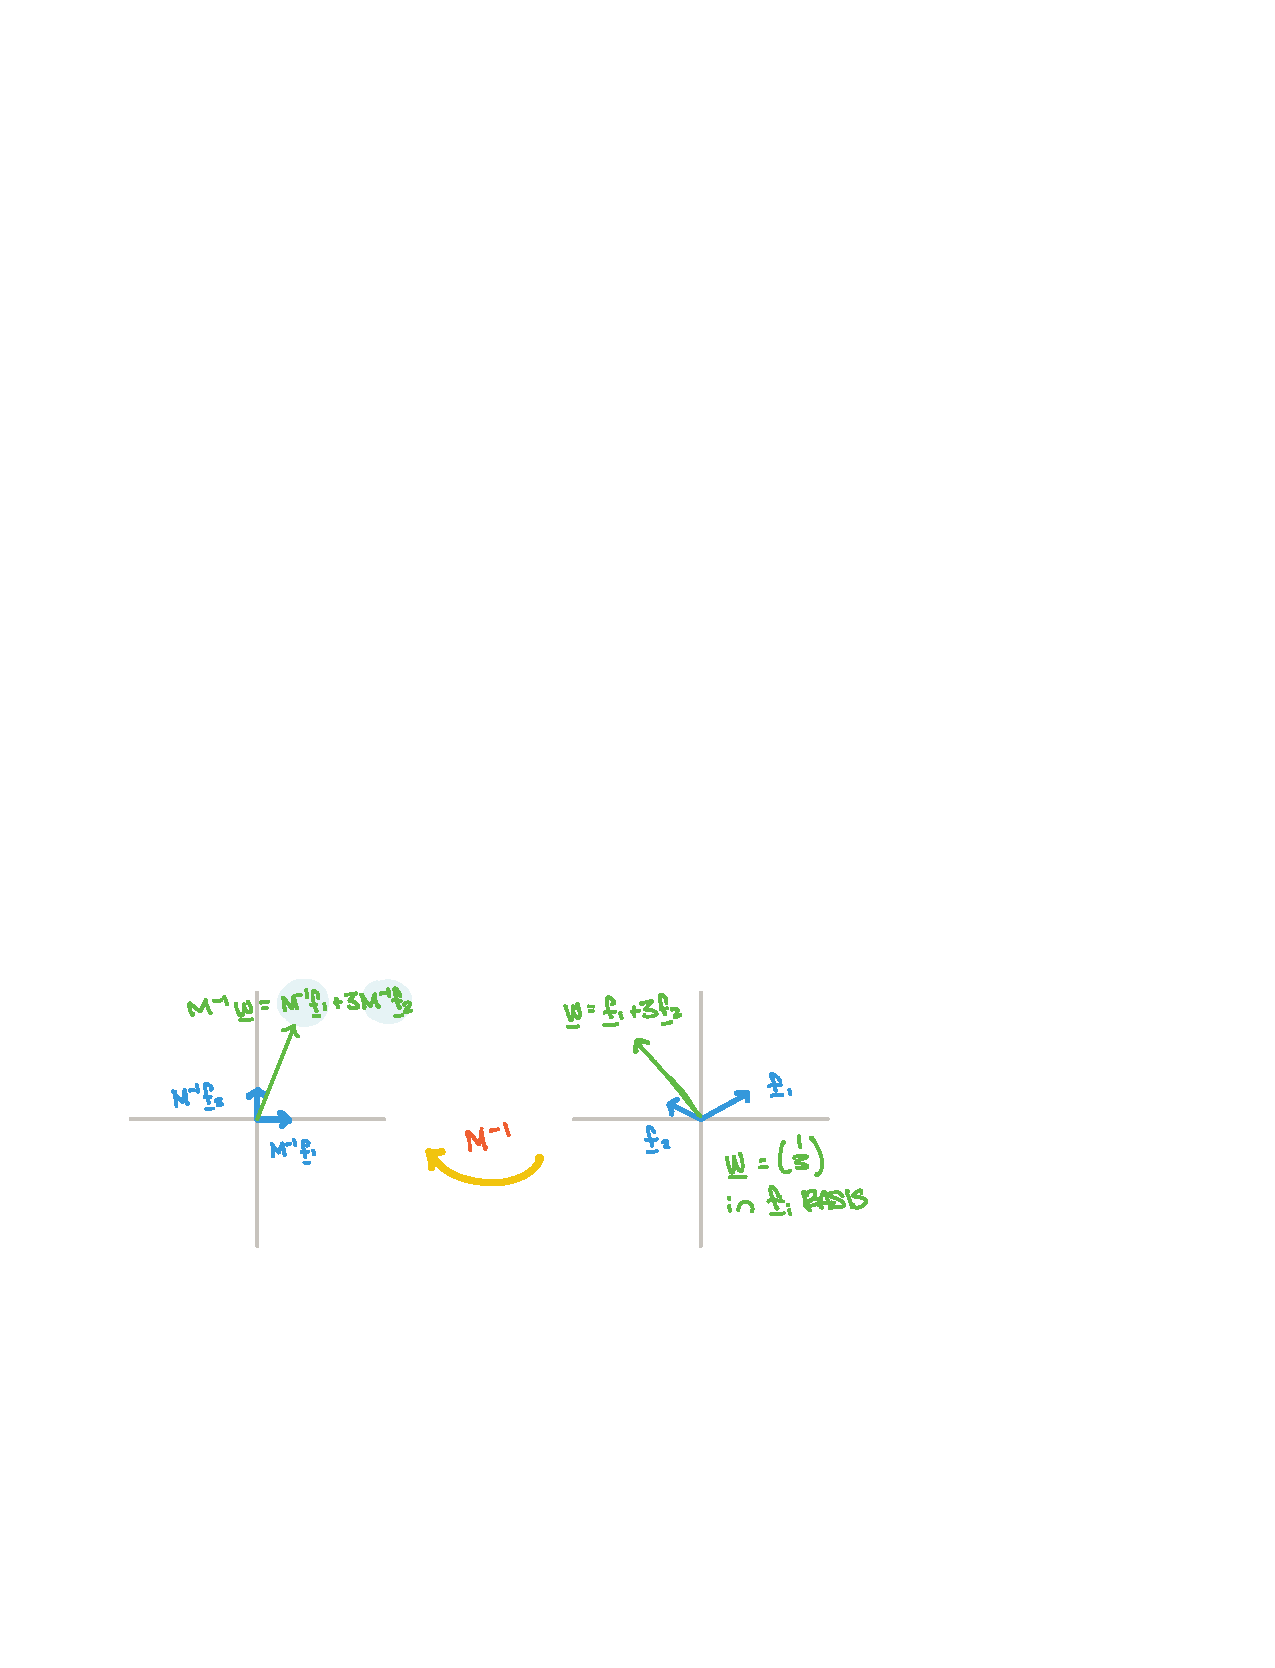
\includegraphics[width=.8\textwidth]{figures/maps_Minv.pdf}
    \caption{Let $M$ is a linear transformation from $\RR ^2 \to \RR ^2$, as we drew in Fig.~\ref{fig:map:M}. Now assume that you have a vector $\vec{w}$ that is the linear combination of some basis vectors $\vec{f}_i$, see the right-hand side of the sketch. If the $\vec{f}_i$ can be obtained as the transformation by $M$ of some other vectors---the basis vectors we called $\bas{e}_i$ in Fig.~\ref{fig:map:M}---then the inverse transformation $M\inv$ acts as a map ``back'' to the original basis. }
    \label{fig:map:M:inv}
\end{figure}

Given a basis, matrices are described by their components, $M\aij{i}{j}$. How do you find the components of the inverse matrix, $(M\inv)\aij{i}{j}$? The most straightforward way is the hard way. Let us consider the $2\times 2$ case. We know that the defining relationship is
\begin{align}
    M(M\inv)=(M\inv)M &= \one 
    &
    M\aij{i}{k}(M\inv)\aij{k}{j}
    =
    (M\inv)\aij{i}{k}M\aij{k}{j} 
    = \delta^i_j \ .
    \label{eq:inverse:matrix:definition}
\end{align}
On the right we have four equations for each combination of $i,j \in\{1,2\}$. We also have four unknown components, $(M\inv)\aij{i}{j}$. This is a system of linear equations that one can usually solve. Sometimes the system will not be solvable---in that case the matrix $M$ is not invertible.

\begin{exercise}
Convince yourself that \eqref{eq:inverse:matrix:definition} holds for \emph{any} vector space of any dimension, $N$. You end up with $N^2$ equations for $N^2$ unknown components $M\aij{i}{j}$. Does this change if all of the components are allowed to be complex numbers?
\end{exercise}


The product of two matrices $M$ and $N$ is a matrix, $MN$. The inverse of the product of matrices is the product of their inverses \emph{in the reverse order}
\begin{align}
    (MN)\inv = N\inv M\inv \ .
\end{align}
You can that this is because you have to undo the transformation that was last applied:
\begin{align}
    (MN)\inv MN = N\inv M\inv MN = N\inv \one  N = \one  \ .
\end{align}




\begin{example}
The inverse of a diagonal matrix is easy:
\begin{align}
    M &=
    \begin{pmatrix}
     3 & \pp  0 \\
     0 & -2
    \end{pmatrix}
    &
    M\inv &=
    \begin{pmatrix}
    \frac{1}{3} & \pp 0 \\
    0 & -\frac{1}{2}
    \end{pmatrix} \ .
\end{align}
We have used the fact that the product of diagonal matrices $\hat M$ and $\hat N$ is also a diagonal matrix whose elements are the products of the corresponding elements in $\hat M$ and $\hat N$.
\end{example}



\subsection{Basis of tensors}

 We may generalize to tensors by writing a generic tensor as:
 \begin{align}
    T =
     T\aij{i_1\cdots i_N}{j_1\cdots j_M}
     \ket{e_{i_1}}\cdots \ket{e_{i_N}}
     \bra{e^{j_1}}\cdots \bra{e^{j_M}} \ .
     \label{eq:tensor:T:with:basis}
 \end{align}
\begin{exercise}
Show how the index rules for tensors contraction onto other objects works using the bra-ket basis notation. Try making up some tensors, say $T^{ij} \ket{e_i}\ket{e_j}$ to see how it can contract onto other objects and use the defining relation \eqref{eq:basis:of:dual:vectors:bra:ket:form} to derive the usual index contractions. 
\end{exercise}

\begin{bigidea}[Tensors as linear functions]\label{idea:tensor:as:function}
Tensors are linear maps from some number of copies of $V$ and $V^*$ to numbers: a $(p,q)$ tensor is a map from $V^q \times (V^*)^p \to \#$. If we write such a tensor as $T\aij{i_1\cdots i_p}{j_1\cdots j_q}$, then these indices may contract with $p$ lower indices and $q$ upper indices to give a number. This is equivalently understood as a \emph{multi-linear} machine that takes in $q$ vectors and $p$ dual vectors to return a number. Here mutli-linear means that the machine is linear in each argument. 
\end{bigidea}

\begin{example}
Consider the $(2,1)$ tensor $T$ with components $T\aij{ij}{k}$. This is a map from $V\times V \times V^* \to \#$ because we may feed it a vector, $v^i$, and two row vectors, $w_j$ and $u_k$ to contract into a number:
\begin{align}
    T(\row{w},\row{u}, \vec{v})
    &=
    T\aij{ij}{k}v^k w_i u_j \ .
\end{align}
\end{example}

\begin{bigidea}[Tensors as linear maps]\label{idea:tensor:as:map}
Tensors are also linear maps between copies of vector spaces and dual vector spaces into other copies of vector spaces and dual vector spaces depending how its indices contract with other objects. A $(p,q)$ tensor $T$ may contract with an $(r,s)$ tensor $S$ such that:
\begin{itemize}
    \item Anywhere 
    \item from 0 to $\min(p,s)$ the upper indices of $T$ are contracted with the pairs of the lower indices of $S$.
    \item Anywhere from 0 to $\min(q,r)$ of the lower indices of $T$ are contracted with the upper indices of $S$.
\end{itemize}
Depending on these choices, the resulting object is a $(m,n)$ tensor where 
\begin{itemize}
    \item $m$ is from $[(p+q) - \min(p,s) - \min(q,r)]$, in the case of maximal contractions, to $(p+q)$, in the case of no contractions.
    \item $n$ is from $[(s+r) - \min(p,s) - \min(q,r)]$, in the case of maximal contractions, to $(s+r)$, in the case of no contractions.
\end{itemize}
\end{bigidea}

\begin{example}[Maps between product spaces]\label{eg:maps:between:product:spaces}
Example~\ref{eg:contraction:choices} and Exercise~\ref{eq:matrix:product:trace} demonstrate this for the case of two (1,1) tensors. 

Consider the case of a $(2,1)$ tensor $T\aij{ij}{k}$. Here are some possible contractions with different kinds of objects (we suppress the basis tensors and only write the components):
\begin{itemize}
    \item $T\aij{ij}{k}v^k$ is a (2,0) tensor $(T\vec{v})^{ij}$.
    \item $T\aij{ij}{k}w_i$ is a (1,1) tensor $(T\row{w})\aij{j}{k}$.
    \item $T\aij{ij}{k}M\aij{k}{\ell}$ is a (2,1) tensor $(TM)\aij{ij}{\ell}$
    \item $T\aij{ij}{k}M\aij{k}{j}$ is a (1,0) tensor $(TM)^i$.
    \item $T\aij{ij}{k}M\aij{\ell}{j}$ is a (2,1) tensor $(TM)\aij{ik}{\ell}$.
    \item $T\aij{ij}{k}T\aij{k\ell}{m}$ is a (3,1) tensor $(T^2)\aij{ij\ell}{m}$.
    \item $T\aij{ij}{k}T\aij{k\ell}{j}$ is a (2,0) tensor $(T^2)^{i\ell}$.
\end{itemize}
As practice, you are welcome to confirm all of this by including the bases `ket-bra' tensors. 
\end{example}

\begin{example}[Why ket-bras?]\label{eg:why:ketbra}
When writing a generic tensor in terms of its basis, say $T$ in \eqref{eq:tensor:T:with:basis}, we typically write these with kets first then bras.\sidenotemark This is a convention that makes it clear that none of the kets are acting on any of the bras.

What if you have a tensor where the order of the indices do not match the kets-first-then-bras convention? For example, a tensor:
\begin{align}
    Y = Y^{ij\phantom{k}\ell}_{\phantom{ij}k}
    \ket{e_i}\otimes\ket{e_j}\otimes\bra{e^k}\otimes\ket{e_\ell} \ ,
\end{align}
where we have used the \sout{X-men} tensor symbol $\otimes$ to make it clear that none of the bras or kets are acting on each other. This avoids any ambiguity, but it is cumbersome to write. (At least not without humming the theme song of the X-men animated series from the 1990s.)

In these cases, it is useful to simply \emph{define} a tensor where the order of indices is more convenient, but that otherwise contains the same information:
\begin{align}
    W = W\aij{ij\ell}{k} 
    \ket{e_i}\ket{e_j} \ket{e_k} \bra{e_\ell}
    \defeq 
    Y^{ij\phantom{k}\ell}_{\phantom{ij}k}
    \ket{e_i} \otimes \ket{e_j} \otimes \bra{e^k} \otimes \ket{e_\ell}
    \ .
\end{align}
This amounts to the component-wise identification
\begin{align}
    W\aij{ij\ell}{k} \equiv Y^{ij\phantom{k}\ell}_{\phantom{ij}k} \ .
\end{align}

\end{example}\sidenotetext{Notationally, kets and bras act on each other when the vertical lines match up, not when their angled parts point at each other.}

Observe that it can sometimes be ambiguous to know which bras and which kets are contracting with one another, so one may have to specify this explicitly. That is: if $T^{ij} \ket{e_i}\ket{e_j}$ is acting on $w_k\bra{e^k}$, which of $\ket{e_i}$ or $\ket{e_j}$ hits the $\bra{e^k}$? 

Practically when one has a tensor with several of the same type of basis bra or ket, one ends up symmetrizing or antisymmetrizing any contraction. This amounts to separating a tensor like $T^{ij} = T^{ij}_\textnormal{s} + T^{ij}_\textnormal{a}$ into a symmetric piece with $T_\textnormal{s}^{ij} = T_\textnormal{s}^{ji}$ and an antisymmetric piece with $T_\textnormal{a}^{ij}=-T_\textnormal{a}^{ji}$. Having done this, it does not matter \emph{which} of the `identical' indices you contract with because they are all treated on the same footing---at least up to a minus sign for the antisymmetric case. See Section~\ref{sec:permutation:symmerty} for the case of two lower indices. This sort of symmetrizing/antisymmetrizing game shows up in the representation theory of symmetries.
% Example: H2 dissociation

\begin{exercise}
Let $B_{ij}\bra{e^i}\bra{e^j}$ be a $(0,2)$ tensor. Separate it into a symmetric and an antisymmetric piece, $B = S+A$ where $S_{ij} = S_{ji}$ and $A_{ij} = - A_{ji}$. Assuming you know each component $B_{ij}$, write out each component $S_{ij}$ and $A_{ij}$.

Let $\vec{v} = v^i\ket{e_i}$ be a vector. Show that $B\ket{v}\ket{v} = S\ket{v}\ket{v}$. That is, show that
\begin{align}
    A\ket{v}\ket{v} = 0 \ .
\end{align}

Let $C^{ij}\ket{e_i}\ket{e_j}$ be an \emph{antisymmetric} $(2,0)$ tensor so that $C^{ij} = C^{ji}$. Show that $BC = AC$, or otherwise that
\begin{align}
    SC = 0 \ .
\end{align}

\textsc{Comment}: in each of these questions, there should be no ambiguity about which bras and which kets are contracted. If you worry that you have to make an arbitrary choice, check that the (anti-)symmetrization means that it does not actually matter up to a minus sign, provided that all objects that have multiple upper and/or multiple lower indices are symmetrized or anti-symmetrized.
\end{exercise}

 

\section{Transformation under symmetries}
\label{sec:transformation:under:symmetries}

Let us return to dancing around the really-big-idea of symmetries, even though we continue to be coy about actually defining these. We first introduced rotations in Section~
\ref{sec:Euclidean:three:space:rotations}, where we pontificated about the relation of rotations to the dot product because rotations leave vector lengths and angles between vectors unchanged. In Section~\ref{sec:isometry:first:pass:indices} we defined Rule~\ref{idea:transformation:of:upper:and:lower:indices} that told us how objects with indices transform. For example, in two-dimensional Euclidean space rotations that move the positive $x$-axis\sidenote{Here I should really say the $\bas{e}_1$ axis rather than the $x$-axis. This is because $x$ and $y$ are typically the coordinates what is called a `base space' or a base \emph{manifold}. In this section we refer to $x,y,$ and $z$ to appeal to our familiarity with three-space.} counter-clockwise (towards the positive $y$ axis) by and angle $\theta$ are $2\times 2$ matrices of the form
\begin{align}
    R(\theta)=
    \begin{pmatrix}
        \cos\theta & -\sin\theta \\
        \sin\theta & \pp \cos\theta
    \end{pmatrix} \ .
\end{align}
The following exercises introduce some of the machinery for rotations.
\begin{exercise}
If you have not done so yet, please confirm that $R(\theta)^\trans = R(\theta)\inv = R(-\theta)$.
\end{exercise}
\begin{example}
In three dimensions there are more kinds of rotations. One way to characterize this is to consider rotations about each coordinate axis. 
\begin{align}
    R_x(\theta) &= 
    \begin{pmatrix}
        1 & & \\
        &  \cos\theta & -\sin\theta \\
        & \sin\theta &  \pp\cos\theta 
    \end{pmatrix}
    \\
    R_y(\theta) &= 
    \begin{pmatrix}
        \pp \cos\theta & &\sin\theta \\
        & 1 & \\
        -\sin\theta& & \cos\theta
    \end{pmatrix}
    \\
    R_z(\theta) &= 
    \begin{pmatrix}
       \cos\theta & - \sin\theta & \\
        \sin\theta &\pp \cos\theta & \\
        & & 1
    \end{pmatrix}\ ,
    \label{eq:3D:rotation:matrices}
\end{align}
where all unlisted components are zero. Notice that these are all reshufflings of the rotations of the plane with the rotation axis held fixed---that should make sense. Also notice that the $R_y(\theta)$ rotation has the $-\sin\theta$ term in the lower-left while the other two rotations have it on the upper-right. This is to consistently apply the right-hand rule convention: a rotation about the $i^\textnormal{th}$ axis corresponds to gripping the axis with your right hand so that your thumb is pointing along the positive direction and identifying the direction that your fingers curl as the rotation direction. For each of these matrices, $R_i(\theta)^\trans = R_i(\theta)\inv = R_i(-\theta)$. 
\end{example}
\begin{exercise}
Taylor expand each of the three matrices in \eqref{eq:3D:rotation:matrices} and write them each in the form
\begin{align}
    R_i(\theta) = \one + i T_i \theta + \mathcal O(\theta^2) \ .
\end{align}
Here $i$ is the imaginary number, $i^2=1$, and the matrix $T_i$ is also pure imaginary.\footnote{This factor of $i$ is a convention in physics.} 

\textsc{Comment:}
The $T_i$ matrices are called \textbf{generators} each type of rotation. Physically, they represent the effect of an infinitesimal rotation about the respective axes. Infinitesimal rotations about other axes are given by \emph{linear combinations} of the $T_i$. In this way, the $T_i$ are a \emph{basis} for rotations.

Show that $T_xT_y - T_y T_x \propto T_z$ and determine the constant of proportionality. This relation is called an \emph{algebra} and denotes the mathematical structure of rotational symmetry.\footnote{This symmetry is called \SO{3}, the special orthogonal group of rank 3. Special means unit determinant, orthogonal means $R^\trans R = \one$.}
\end{exercise}

\begin{exercise}
The \emph{generator} of \SO{2}, rotations of the Euclidean plane, is
\begin{align}
    T = \begin{pmatrix}
        0 & i \\
        -i & 0
    \end{pmatrix} \ .
\end{align}
Show that $R(\theta) = \exp(iT\theta)$ where the matrix exponential is defined as its power series:
\begin{align}
    e^{M} = 1 + M + \frac{1}{2}M^2 + \cdots \ .
\end{align}
Use the power series expansion of the trigonometric functions. 
\end{exercise}

Assuming that we have a definition for which transformations are rotations,\sidenote{More generally, which transformations are \emph{isometries}. We finally present such a definition in Chapter~\ref{ch:metric:spaces}.} then we can examine how the basis vectors and row vector transform.

% Motivating the indices
% What is a symmetry



\subsection{Transformation of Vectors}\label{sec:active:passive}

To be somewhat philosophical: under an isometry like a rotation, there are two pictures to think about what happens to a vector:
\begin{itemize}
    \item \textbf{Active transformation}\index{active transformation}: your basis vectors stay put, but the vector is changing into a different vector, $\ket{v} \to \ket{v'}$. The components of $\ket{v'}$ are clearly different from the components of $\ket{v}$ because it the two are simply not the same vector.
    \item \textbf{Passive transformation}\index{passive transformation}: the vector \emph{does not change}, but the basis vectors change, $\ket{e_i} \to \ket{e'_i}$. This means that the components of $\ket{v}$ must \emph{also} change so that $v^i\ket{e_i} = v'^{i}\ket{e_i}$.
\end{itemize}
In an active transformation, the vector space and every vector in it change. In a passive transformation, the observer changes.\sidenote{There is something oddly Zen and philosophical about this.} For an isometry---a symmetry of the system---either perspective is valid. See Figures~\ref{fig:do:something} and \ref{fig:passive:rotation}.
% 

\begin{figure}[tb]
    \centering
    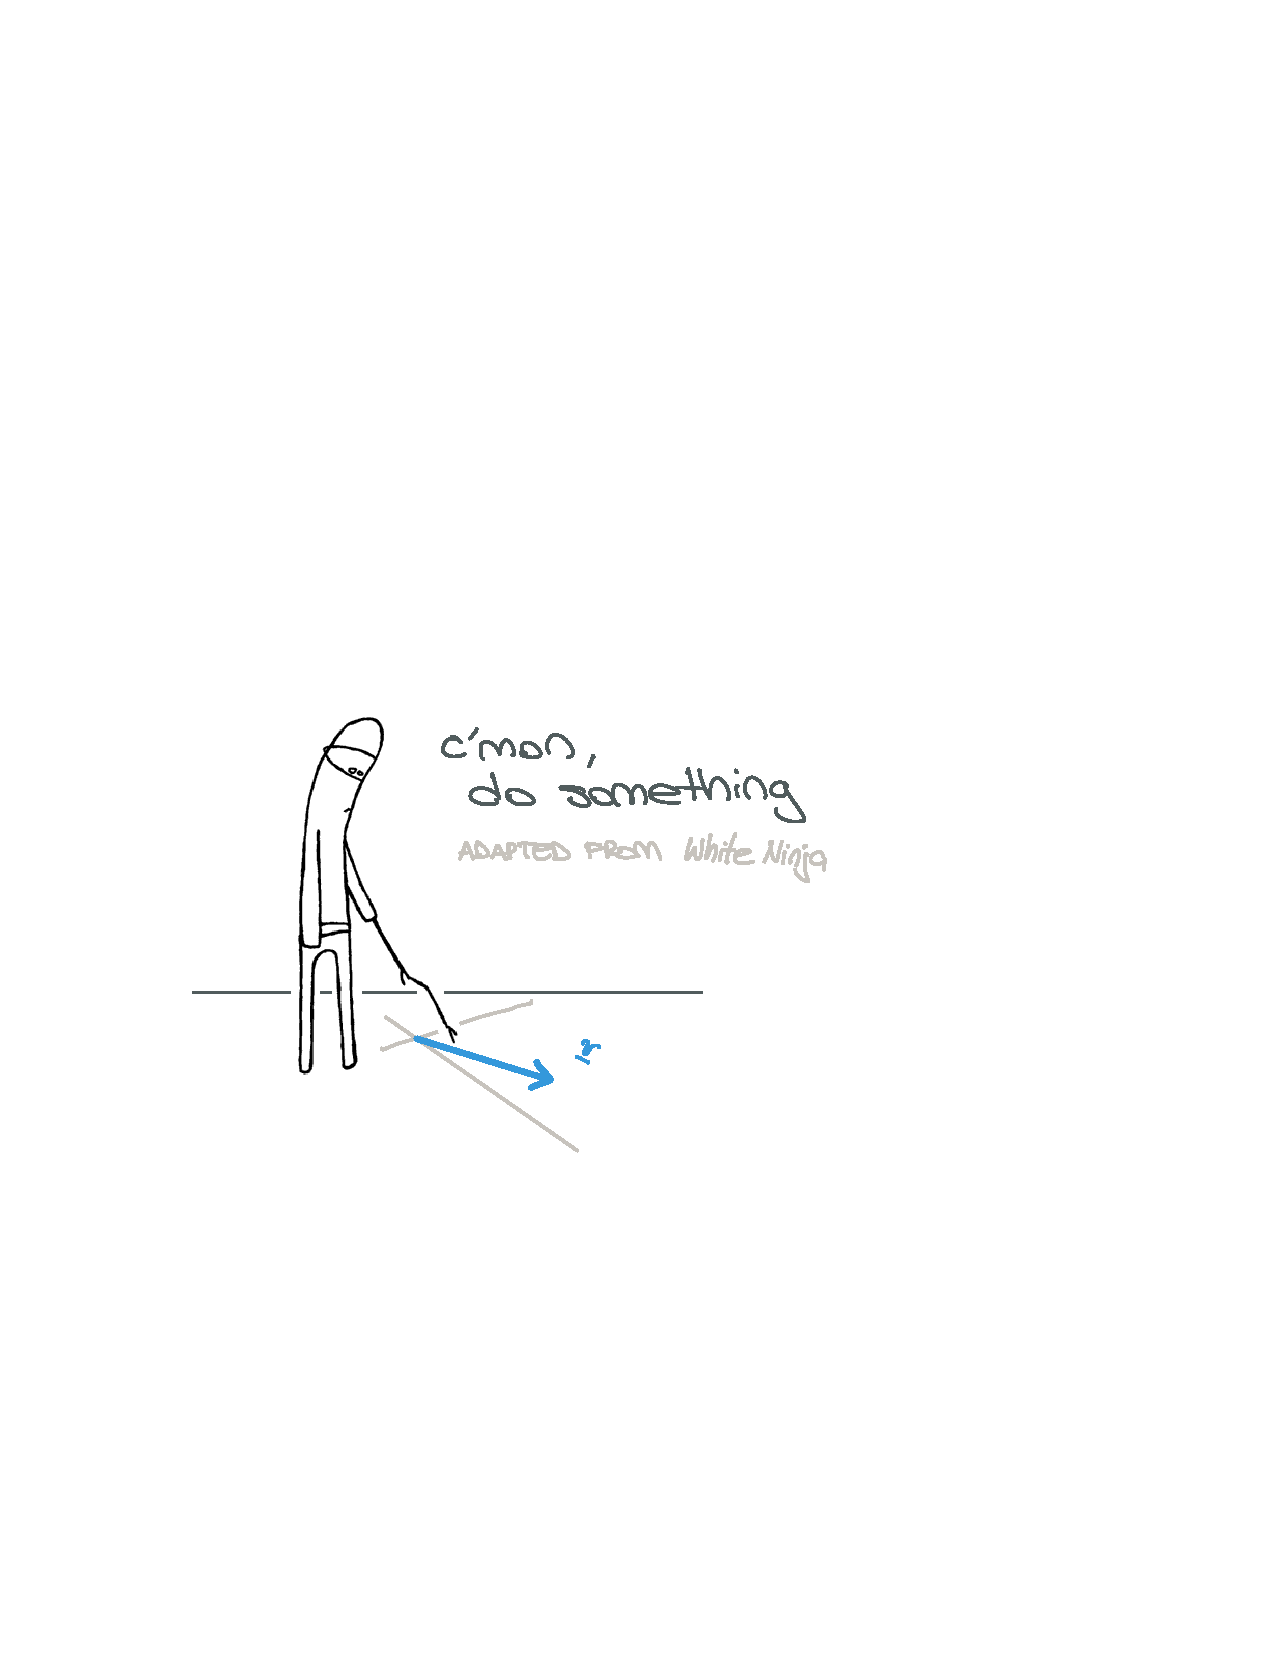
\includegraphics[width=.5\textwidth]{figures/passivetransform_dosomething.pdf}
    \caption{
        Nothing actually happens during a passive transformation. The basis vectors transform, but the components of the vector transform in such a way that $v'^i\bas{e}'_i = v^i\bas{e}_i$. Such a `transformation' may come off as uninspiring, but this is the basis of symmetries in physics. 
        From \url{https://knowyourmeme.com/memes/cmon-do-something}.
    }
    \label{fig:do:something}
\end{figure}

\begin{figure}[tb]
    \centering
    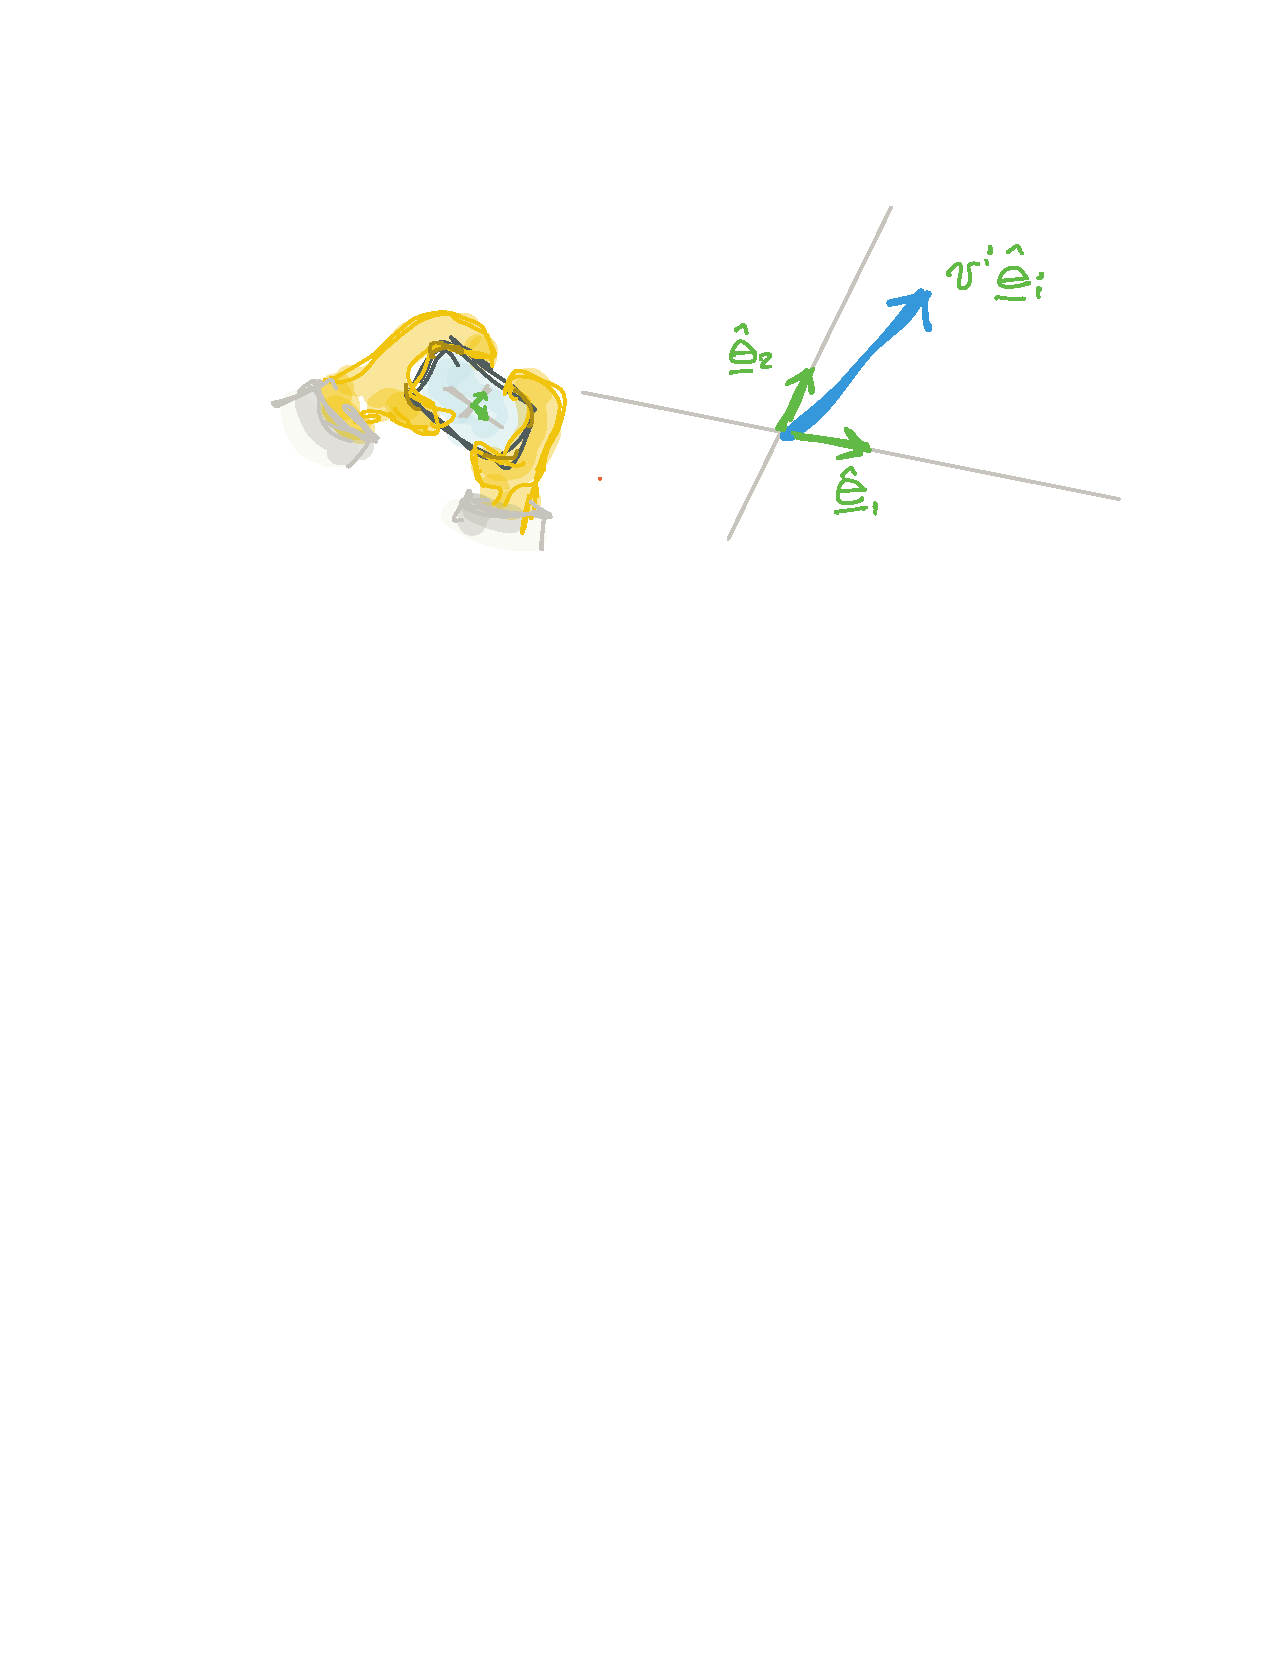
\includegraphics[width=.43\textwidth]{figures/rotate_1.pdf}
    \quad\quad
    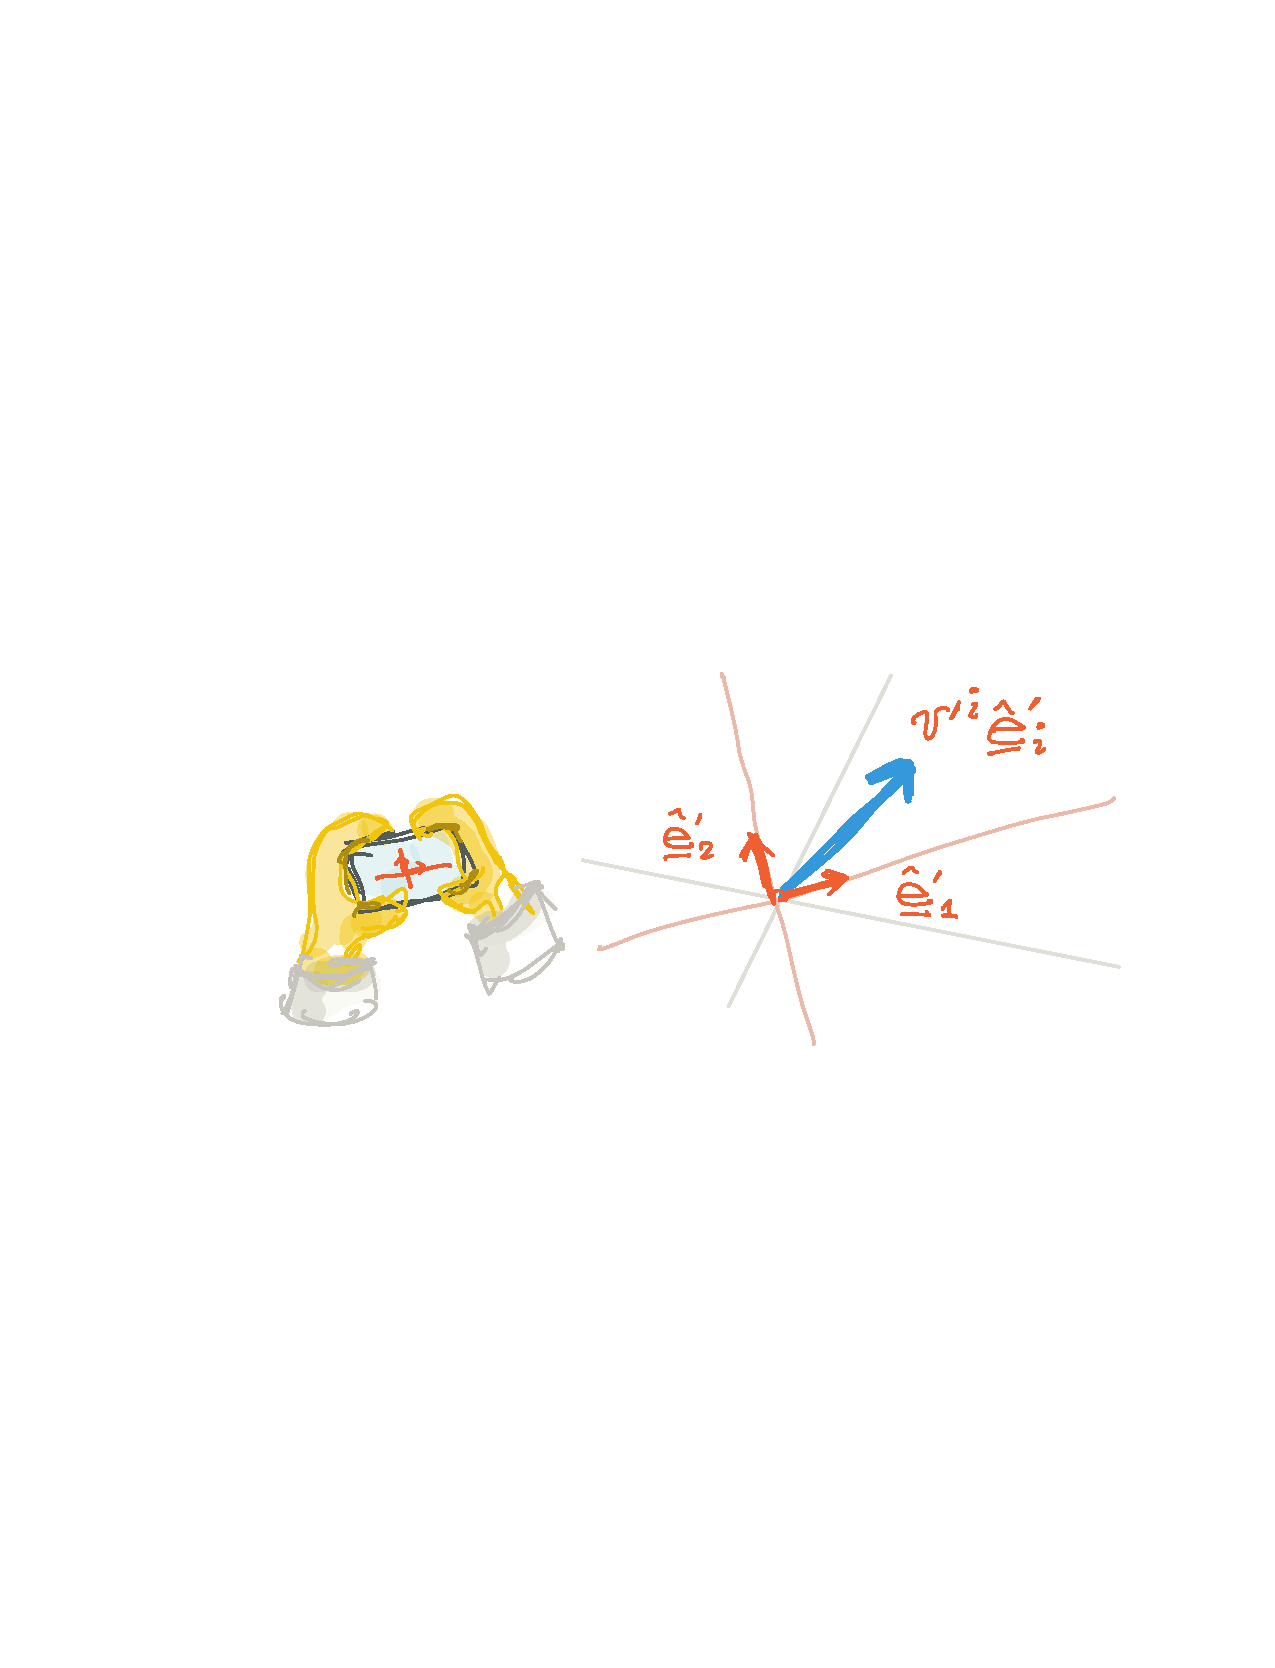
\includegraphics[width=.43\textwidth]{figures/rotate_2.pdf}
    \caption{Example of a passive rotation. You are looking at a vector $\vec{v}$ through your phone. The image on your phone has a natural orientation for a basis $\bas{e}_i$ and the components of $\vec{v}$ in this basis are $v^i$. You could also rotate your phone, leaving the vector $\vec{v}$ untouched. The new basis vectors are $\bas{e}_i'$; they are different from $\bas{e}_i$ because your phone has changed orientation. With respect to the new basis, the same vector $\vec{v}$ now has components $v'^i$.}
    \label{fig:passive:rotation}
\end{figure}

Let $R(\theta)$ be the rotation about some axis by some angle $\theta$ that enacts a symmetry transformation. In the passive picture, vectors remain unchanged, but the basis vectors and the corresponding components do change:
\begin{align}
    \ket{v} = v^i \ket{e_i} =
    % v^i R\inv R \ket{e'_i}
    v^\ell R\aij{i}{\ell} (R\inv)\aij{\ell}{k}  \ket{e_k} \
    \defeq (v')^\ell \ket{e'_\ell}
    \ .
\end{align}
In the second equality we have simply inserted $\one = R R\inv$. On the right-hand side we \emph{define} the rotated components $v'$ and rotated basis vectors $\ket{e'}$ by absorbing the $R$ and $R\inv$ rotations:
\begin{align}
    (v')^i &\defeq R\aij{i}{\ell} v^\ell
    &
    \ket{e'_i} &\defeq  (R\inv)\aij{j}{i}\ket{e_j} \ .
    \label{eq:passive:transformation:of:vector:and:basis}
\end{align}
All we have done is collect into $v'^i$ all objects that contract with $v^ell$ and leave an object of a single upper index: that means that we absorb the $R\aij{i}{\ell}$. Similarly, we collect into $\ket{e'_i}$ all objects that contract with $\ket{e_j}$ and leave an object of a single lower index: that means we absorb the $(R\inv)\aij{j}{i}$. From this we have \emph{derived} the ``indexology rule'' \eqref{eq:components:of:vector:and:row:under:rotatino} which led us to the general tensor transformation in \bigidearef{}~\ref{idea:transformation:of:upper:and:lower:indices}.

Let me say that one more time: in \eqref{eq:passive:transformation:of:vector:and:basis} we are not \emph{applying} the rule that upper indices transform with $R$ and lower indices transform with $R\inv$. In fact, we are \emph{deriving it} from the condition that a passive [symmetry] transformation leaves the vector $\ket{v}$ unchanged while simply changing the basis and components of $\ket{v}$ while preserving $\ket{v}$.



To be clear, this choice of active versus passive pictures is only true for symmetries (isometries) where in some sense the system is not meaningfully changing. A general transformation that is \emph{not} an isometry should be thought of as an active transformation that change vectors.
\begin{example}
If we were to rotate the entire solar system, then it does not matter too much whether we think about this as some cosmic entity actually changing the configuration of every celestial object \emph{or} if we simply choose a rotated set of coordinates for the solar system. However, if we were to \emph{stretch} the solar system along one axis of the plane of the planets' rotation, then all of a sudden the planets would not be in stable orbits.\sidenotemark
\end{example}\sidenotetext{In this hypothetical: the coordinates do not change and Newton's laws do not change. Thus stretching the positions of each of the plants pulls them further away from the center of the sun without changing their angular momentum.}


\subsection{Transformation of Row Vectors}

The same argument holds for row vectors. For an isometry, one may take the passive transformation perspective in which row vectors do not transform, but we transform both the basis row vectors $\bra{e^i}$ and components of the row vector $w_i$ in such a way that $\bra{e^i}w_i \to \bra{{e'}^i}w'_i = \bra{w}$: 
\begin{align}
    w'_i &\defeq \tilde R\aij{\ell}{i} w_\ell
    &
    \bra{e'^i} &\defeq  (\tilde{R}\inv)\aij{i}{j}\bra{e^j} \ .
    \label{eq:passive:transformation:of:row:vector:and:basis}
\end{align}
In principle, this rotation $\tilde R$ is a different rotation from $R$. One may think think that $\tilde R$ has \emph{nothing to do} with the transformation of vectors, $v^i\ket{e_i} \to R\aij{i}{k}v^k(R\inv)\aij{\ell}{i}\ket{e_\ell}$. However, if $R$ and $\tilde R$ enact a symmetry of the system, then the transformations must preserve the defining relation of the dual vector basis \eqref{eq:basis:of:dual:vectors}, or the bra-ket form of that rule \eqref{eq:basis:of:dual:vectors:bra:ket:form}. This means we want to impose
\begin{align}
    \la e'^i \mid e'_j \ra \equiv \delta^i_j \ .
    \label{eq:basis:transform:under:rotation}
\end{align}
Inserting our expressions of the passively rotated basis elements relative to the original basis elements,\sidenote{We do this because we assume that the original basis elements satisfy $\la e^i \mid e_j \ra \equiv \delta^i_j$.}
\begin{align}
    \la e'^i \mid e'_j \ra &= 
    \la e^k \mid (\tilde{R}\inv)\aij{i}{k} (R\inv)\aij{\ell}{j} \mid e_\ell \ra
    =
    (\tilde{R}\inv)\aij{i}{k} (R\inv)\aij{\ell}{j} \la e^k \mid e_\ell \ra
    \\
    &=
    (\tilde{R}\inv)\aij{i}{k} (R\inv)\aij{\ell}{j} \delta^k_\ell
    =
    (\tilde{R}\inv)\aij{i}{k} (R\inv)\aij{k}{j} \ .
\end{align}
In order for this to equal $\delta^i_j$ we must have
\begin{align}
    (\tilde R)\inv R\inv = \one \ ,
\end{align}
or equivalently
\begin{align}
    \tilde R = R\inv \ ,
\end{align}
which is precisely what we motivate below \eqref{eq:R:Rtilde:transformation:from:indices:rotation}. 


\subsection{Transformation of Tensors}

Having established how $\ket{e_i}$ and $\bra{e^j}$ transform, the transformation of a general tensor---one composed of the tensor product of some number of bras and some number of kets---follows simply from the transformation of each bra and ket individually.

\begin{wide}
In this way, we may augment Rule~\ref{idea:transformation:of:upper:and:lower:indices} and \eqref{eq:transformation:of:upper:and:lower:indices} with the statement that from the passive transformation perspective, the basis tensors transform as
\begin{align}
    % T\aij{i_1\cdots i_N}{j_1\cdots j_M}
    % \to 
    % R\aij{i_1}{k_1}\cdots R\aij{i_N}{k_N}
    % (R\inv)\aij{\ell_1}{j_1}\cdots (R\inv)\aij{\ell_N}{j_N}
    % T\aij{k_1\cdots k_N}{\ell_1\cdots \ell_M} \ .
    % \label{eq:transformation:of:upper:and:lower:indices}
    \ket{e_{i_1}} \cdots \ket{e_{i_N}}
    \bra{e^{j_1}} \cdots \bra{e^{j_M}}
    \to 
    (R\inv)\aij{k_1}{i_1}\cdots (R\inv)\aij{k_N}{i_N}
    R\aij{j_1}{\ell_1}\cdots R\aij{j_N}{\ell_M}
    \ket{e_{k_1}} \cdots \ket{k_{i_N}}
    \bra{e^{\ell_1}} \cdots \bra{e^{\ell_M}} \ .
\end{align}
For completeness, here is how the components transform:
\begin{align}
    T\aij{i_1\cdots i_N}{j_1\cdots j_M}
    \to 
    R\aij{i_1}{k_1}\cdots R\aij{i_N}{k_N}
    (R\inv)\aij{\ell_1}{j_1}\cdots (R\inv)\aij{\ell_M}{j_M}
    T\aij{k_1\cdots k_N}{\ell_1\cdots \ell_M} \ .
    \tag{\ref{eq:transformation:of:upper:and:lower:indices}}
\end{align}
\end{wide}

Let us observe that the rule we proposed in Rule~\ref{idea:transformation:of:upper:and:lower:indices} is simply a \emph{byproduct} of our definition of how the basis bras and kets transform. In fact, it is the product of the definition of how \emph{either} the basis bras or the basis kets transform, since the transformation law of the other type of object necessarily follows from \eqref{eq:basis:transform:under:rotation}.

\begin{example}[Moment of inertia]
The moment of inertia tensor has two lower indices.\footnote{This may depend on conventions. It is certainly true that the moment of inertia tensor has two indices that are both the same height.} Explain why it transforms differently from a matrix, which has one upper and one lower index.
\end{example}

\subsection{(Non-)Transformation of Numbers}

Numbers---perhaps you want to call them scalars---do not transform. They have no free indices to transform. Some numbers have contracted indices. Consider a bra $\bra{w}$ acting on $M$, which in turn acts on a $\ket{v}$,\sidenote{You can alternatively say that $M$ is acted on by both $\bra{w}$ and $\ket{v}$, or many other combinations.}
\begin{align}
    \la w \mid M \mid v \ra 
    &= 
    w_i \bra{e^i} \; M\aij{j}{k}\ket{e_j}\!\bra{e^k}
    \; v^\ell \ket{e_\ell} 
    \\&=
    w_i M\aij{i}{k}v^k 
    \ ,
\end{align}
where we have used the defining relation $\la e^i\mid \ra e_j = \delta^i_j$. These combinations are invariant and no longer transform. That's why we may use the $\delta$ function to collapse sums. We are left with a transformation law
\begin{align}
    w_i M\aij{i}{k}v^k 
    \to 
    w_\ell(R\inv)\aij{\ell}{i} \, R\aij{i}{m}
    M\aij{m}{n} (R\inv)\aij{n}{k} \, R\aij{k}{p} v^p \ .
\end{align}
We find two instances of the contraction $(R\inv)\aij{a}{b}R\aij{b}{c} \equiv \delta^a_c$, which shows that the right-hand side is identical to the left-hand side. In this way an object whose indices are fully contracted does not transform. 

\begin{exercise}
Analogously, an object with some contracted indices and some uncontracted indices \emph{does} transform, but only according to the uncontracted indices. If $T_{ik}$ is a (0,2) tensor, show that $T_{ik}v^k$ transforms like a row vector by transforming each pf $T_{ik}$ and $v^k$ independently and showing that one factor of $R$ and one factor of $R\inv$ cancel each other out.
\end{exercise}




\section{Dropping the Basis Tensors... Again}

In Section~\ref{sec:component:notation} we presented tensors the way that most physicists use tensors: objects with indices. In the rest of this chapter, we built up the machinery of basis linear maps that form the underlying structure of what tensors are. This helps us understand how the components of a tensor transform when we change basis. By virtue of the defining relation between basis bras and kets, \eqref{eq:defining:bra:ket:relatin}, you may have found that once we all agree upon a basis, then \emph{all of those basis tensors are kind of redundant}!

In other words, when there is no ambiguity about basis, I could have just written $v^i$ and you would \emph{know} that the only possible thing that I could mean is $v^i\ket{e_i}$. Similarly, the matrix $M\aij{i}{j}$ could \emph{only} possibly mean $M\aij{i}{j}\ket{e_i}\!\bra{e^j}$. This is because we know that all of these objects are intrinsically index-free---the indices all contract with the appropriate basis objects. This then leads us to the idea that maybe we could just \emph{drop} the basis tensors and just write everything as objects with indices.

Everything we have said in this chapter is still true and still \emph{under the hood}, so to speak. But you will find that physicists find it most convenient to work in the shorthand of just writing the \emph{components} of tensors with the implicit understanding of there being a contraction with basis tensors.\footnote{Roger Penrose proposes formalizing this shorthand in what is called \emph{abstract index notation}. A good online discussion is this one: \url{https://math.stackexchange.com/questions/455478/}} 



\begin{subappendices}


\section{Permutation Symmetry}\label{sec:permutation:symmerty}

Our favorite objects thus far---vectors, dual vectors, and matrices---have been refreshingly \emph{unambiguous} in the following sense: If you are looking to contract indices, you know \emph{exactly} which indices can contract. An ambiguity arises when we have a tensor that has multiple upper or lower indices. Consider the following example of a (0,2) tensor $A$ acting on a vector $\ket{v}$:
\begin{align}
    B_{ij}\bra{e^i}\bra{e^j} \; v^k \ket{e_k} \ .
\end{align}
The following two statements are equivalent:
\begin{itemize}
    \item There is an ambiguity about which of the two bras, $\bra{e^i}$ or $\bra{e^j}$, contracts with the basis ket $\ket{e_k}$. 
    \item In the shorthand where we do not write the basis tensors, there is an ambiguity about which of the lower $i$ or $j$ indices of the matrix $B$ contracts with the upper index of the $\vec{v}$.
\end{itemize}
\begin{exercise}
Show that both of these statements are equivalent by using \eqref{eq:defining:bra:ket:relatin}. 
\end{exercise}
One way to break the degeneracy is to explicitly specify \emph{which} contraction we really want---this is in the spirit of Example~\ref{eg:contraction:choices}. There is a trick that we often employ: take symmetric and antisymmetric combinations of the indices.

For our purposes, let us stick to the case of tensors with two lower indices like $B$ above. The trick is to separate the components of $B$ into a symmetric and an antisymmetric part:
\begin{align}
    B_{ij} &= S_{ij}+A_{ij}
\end{align}
where these pieces are 
\begin{align}
    S_{ij} &= \frac{1}{2} \left(B_{ij} + B_{ji}\right)
    \\
    A_{ij} &= \frac{1}{2} \left(B_{ij} - B_{ji}\right) \ .
\end{align}
\begin{exercise}
Decompose the (0,2) tensor $B_{ij}$ below\footnote{For ease of notation we have written the components of $B_{ij}$ as a square array of numbers. This does not mean that $B$ is a matrix---at least not in the sense of being a (1,1) tensor. This is simply for notation. When writing out the components of any two-index tensor in ``matrix multiplication'' notation, there is no way to distinguish between (2,0), (1,1), and (0,2) tensors.} into its symmetric and antisymmetric parts:
\begin{align}
    \begin{pmatrix}
        B_{11} & B_{12}\\
        B_{21} & B_{22}
    \end{pmatrix}
    =
    \begin{pmatrix}
        1 & 2\\
        0 & 3
    \end{pmatrix} \ .
\end{align}
\end{exercise}


\begin{exercise}
A basis of symmetric and antisymmetric (0,2)-tensors are:
\begin{align}
    \la{e^{(i}}|\la{e^{j)}}|
    \defeq&
    \frac{1}{2}\left( 
        \bra{e^i}\bra{e^j} + \bra{e^i}\bra{e^j}
    \right)
    \\
    \la{e^{[i}}|\la{e^{j]}}|
    \defeq&
    \frac{1}{2}\left( 
        \ket{e^i}\bra{e^j} - \ket{e^i}\bra{e^j}
    \right) \ .
\end{align}
The factor of $1/2$ is conventional. The subtle curved-versus-square bracket notation is also a standard convention. How would you perform the projection that takes $(0,2)$ tensors into their symmetric parts? What about their antisymmetric parts?

Show that if $S_{ij} = S_{ji}$ is symmetric, then 
\begin{align}
     S_{ij}\la{e^{[i}}|\la{e^{j]}}| = 0 \ .
 \end{align}
\end{exercise}


The symmetric tensor is especially nice:
\begin{quote}
When contracting a symmetric tensor $S_{ij}$ with a vector, it does not matter which index one contracts with. 
\end{quote}
Let us see this in action\sidenote{We simply contract components---if you want, you can write this in full bra-ket notation with the basis tensors written out. It is a good exercise if you are not used to it.}:
\begin{align}
    S_{ij}v^j = S_{ji}v^j \ .
\end{align}
We use the symmetry of $S$ to show that we could have equivalently contracted with the first index or the second. Note that the free index needs to remain the same in order for the equality to make sense: we are looking at the $i^\text{th}$ component of $S\ket{v}$.

We can see this in action for a contraction with two vectors as well:
\begin{align}
    S_{ij}v^iw^j = S_{ji}v^i w^j = S_{ij} v^j w^i \ .
    \label{eq:symmetric:with:two:vectors}
\end{align}
In the last equality we simply relabel the contracted (`dummy') indices.

The antisymmetric tensor is also nice, though slightly less so. Here we have
\begin{align}
    A_{ij}v^j = - A_{ji}v^j \ .
\end{align}
The effect of whether we contract with the first or the last index is an overall minus sign. For a double contraction:
\begin{align}
    A_{ij}v^iw^j = -A_{ji}v^i w^j = -A_{ij} w^i v^j \ .
\end{align}
In the last line we have deliberately swapped the order of $w^i v^j$---which commute---to make this look suggestively similar to the cross product. \flip{To fill in: connection of Levi-Civita symbol to cross product in three dimensions.}





\begin{exercise}
Convince yourself that all of our discussion here holds for tensors with two upper indices. Further, convince yourself that the discussion holds if $B$ happened to also have an upper index: $B\aij{i}{jk}$. Finally, convince yourself that if $B$ had two upper and two lower indices, $B\aij{ij}{k\ell}$, one could separately symmetrize and antisymmetrize each index.
\end{exercise}



\section{\texorpdfstring{The Kronecker $\delta$}{The Kronecker Delta}}\label{sec:kronecker}

The Kronecker $\delta$ is defined to be
\begin{align}
    \delta^i_j = 
    \begin{cases}
        1 &\text{ if }i=j \\
        0 &\text{ otherwise}
    \end{cases} . 
\end{align}
A useful way to think of this is that $\delta^i_j$ are the components of the identity matrix:
\begin{align}
    \one = \delta^i_j \ket{e_i}\bra{e^j} \ .
\end{align}
Unlike typical matrix components, we write the indices vertically aligned because there is no ambiguity about the ordering: any component for which the ordering matters is already zero.\sidenote{This makes the $\delta^i_j$ stick out a bit as if it were reminding us that \emph{hey, I'm just the identity}. Most likely we just use this convention because it is easier to type up in \LaTeX.}

Think of $\delta^i_j$ as a tool to collapse sums.
\begin{example}
Consider the contraction $\delta^i_j v^j$. Expanding this gives:
\begin{align}
    \delta^i_j v^j = 
    \delta^i_1 v^1
    +
    \delta^i_2 v^2
    +
    \delta^i_3 v^3
    + 
    \cdots
\end{align}
For any specific $i$, only one of the terms is non-zero. For example,
\begin{align}
    \delta^{i=2}_j v^j = 
    \cancel{\delta^2_1} v^1
    +
    \delta^2_2 v^2
    +
    \cancel{\delta^i_3} v^3
    + 
    \cdots
    = 
    v^2 \ .
\end{align}
\end{example}


\begin{example}\label{eq:double:sum:delta}
Consider the double sum $w_i \delta^i_j v^j$ \ .
\begin{align}
    w_i \delta^i_j v^j = &
    \pp w_1 \delta^1_1 v^1 + w_1 \cancel{\delta^1_2} v^2 + \cdots \\
    &+ w_2 \cancel{\delta^2_1} v^1 + w_2 \delta^2_2 v^2 + \cdots \\
    =& w_1v^1 + w_2 v^2 + \cdots = w_iv^i \ .
\end{align}
\end{example}

The example above gives us a rule to use the Kronecker $\delta$ to collapse sums:
\begin{newrule}
Whenever the $j$ index in $\delta^i_j$ contracts with the upper index of a tensor, you can simply replace that upper index with the $i$ from the $\delta^i_j$. Similarly, whenever the $i$ index in $\delta^i_j$ contracts with the lower index of a tensor, you can simply replace that lower index with the $j$ from the $\delta^i_j$.
\end{newrule}

\begin{example}
Consider the contraction between two general tensors:
\begin{align}
    S\aij{i_1\cdots i_N i}{j_1\cdots j_M} T\aij{k_1\cdots k_P}{\ell_1\cdots \ell_Q \ell}
    \delta^\ell_i &= 
    S\aij{i_1\cdots i_N i}{j_1\cdots j_M} T\aij{k_1\cdots k_P}{\ell_1\cdots \ell_Q i}
    \\
    &=
    S\aij{i_1\cdots i_N \ell}{j_1\cdots j_M} T\aij{k_1\cdots k_P}{\ell_1\cdots \ell_Q \ell}\ ,
\end{align}
where in the second line we simply show that it does not matter whether you replace the upper or lower index.
\end{example}


\begin{example}
Sometimes it is helpful to see something written in gory detail. Let us write out even more terms in Example~\ref{eq:double:sum:delta}:
\begin{align}
    w_i \delta^i_j v^j = 
    &
    \pp w_1 \delta^1_1 v^1 
    + w_1 \cancel{\delta^1_2} v^2 
    + w_1 \cancel{\delta^1_3} v^3 
    + w_1 \cancel{\delta^1_4} v^4 
    + \cdots 
    \\
    & 
    + w_2 \cancel{\delta^2_1} v^1
    + w_2 {\delta^2_2} v^2 
    + w_2 \cancel{\delta^2_3} v^3 
    + w_2 \cancel{\delta^2_4} v^4 
    + \cdots 
    \\    & 
    + w_3 \cancel{\delta^3_1} v^1
    + w_3 \cancel{\delta^3_2} v^2 
    + w_3 {\delta^3_3} v^3 
    + w_3 \cancel{\delta^3_4} v^4 
    + \cdots 
    \\    & 
    + w_4 \cancel{\delta^4_1} v^1
    + w_4 \cancel{\delta^4_2} v^2 
    + w_4 \cancel{\delta^4_3} v^3 
    + w_4 {\delta^4_4} v^4 
    + \cdots 
    \\
    = &
    \pp w_1 \delta^1_1 v^1 
    \phantom{+ w_1 \cancel{\delta^1_2} v^2 }
    \phantom{+ w_1 \cancel{\delta^1_3} v^3 }
    \phantom{+ w_1 \cancel{\delta^1_4} v^4 }
    \phantom{+ \cdots }
    \\
    & 
    \phantom{+ w_2 \cancel{\delta^2_1} v^1}
    + w_2 {\delta^2_2} v^2 
    \phantom{+ w_2 \cancel{\delta^2_3} v^3 }
    \phantom{+ w_2 \cancel{\delta^2_4} v^4 }
    \phantom{+ \cdots }
    \\    & 
    \phantom{+ w_3 \cancel{\delta^3_1} v^1}
    \phantom{+ w_3 \cancel{\delta^3_2} v^2 }
    + w_3 {\delta^3_3} v^3 
    \phantom{+ w_3 \cancel{\delta^3_4} v^4 }
    \phantom{+ \cdots }
    \\    & 
    \phantom{+ w_4 \cancel{\delta^4_1} v^1}
    \phantom{+ w_4 \cancel{\delta^4_2} v^2 }
    \phantom{+ w_4 \cancel{\delta^4_3} v^3 }
    + w_4 {\delta^4_4} v^4 
    + \cdots 
    % & w_1v^1 + w_2 v^2 + \cdots = w_iv^i 
    \\
    =& w_1v^1\phantom{\delta^i_j} + w_2 v^2\phantom{\delta^i_j} + w_3 v^3\phantom{\delta^i_j} + w_4 v^4\phantom{\delta^i_j} \cdots 
    \\=& w_iv^i 
    \ .
\end{align}
The key here is to first understand why several terms are zero, then to learn the `rule of thumb' that the $\delta^i_j$ reduces a double sum into a single sum. Any time you have a repeated index where one of the repeated indices is on a Kronecker-$\delta$, you can simply remove the Kronecker $\delta$ and replace that index with the \emph{other} index on $\delta$. In the example above, we saw that there was a repeated $j$ index in $w_i \delta^i_j v^j$. We found that we can simply remove the $\delta$ and replace the $v^j$ with $v^i$ because $i$ is the `other' index on $\delta^i_j$.
\end{example}

\section{Canceling factors in a tensor equation}

\begin{wide}
Sometimes you will find equations of the following form:
\begin{align}
    w_i M\aij{i}{j}v^j = w_i A\aij{i}{j}v^j \ .
    \label{eq:canceling:factors:wMv}
\end{align}
If we were to expand this, the equation reads:
\begin{align}
    w_1 M\aij{1}{1}v^1 + w_1 M\aij{1}{2}v^2
    + w_2 M\aij{2}{1}v^1 + w_2 M\aij{2}{2}v^2
    =
    w_1 A\aij{1}{1}v^1 + w_1 A\aij{1}{2}v^2
    + w_2 A\aij{2}{1}v^1 + w_2 A\aij{2}{2}v^2 \ ,
    \label{eq:canceling:factors:wMv:long}
\end{align}
where we take the two-dimensional case for brevity. 
\end{wide}

Based on this equation, can you infer anything about how the matrices $M$ and $A$ relate to one another? Not by itself since the equation seems to depend on the values of $w_i$ and $v^j$. 

However, if we further said that \eqref{eq:canceling:factors:wMv} is true \emph{for any vector $\vec{v}$ and any dual vector $\row{w}$}, then we can deduce that 
\begin{align}
    M\aij{i}{j} = A\aij{i}{j} \ ,
\end{align}
the two matrices are equivalent. This is clear in the expanded form of the equation. If you set $w_1 = v^2 = 1$ while $w_2 = v^1 = 0$, then \eqref{eq:canceling:factors:wMv:long} reduces to $M\aij{1}{2} = A\aij{1}{2}$. You can do this for any choices of the $\row{w}$ and $\vec{v}$ components. This leads us to want to take \eqref{eq:canceling:factors:wMv} and \emph{cancel} the common factors on both sides:
\begin{align}
    \cancel{w_i} M\aij{i}{j} \cancel{v^j} = \cancel{w_i} A\aij{i}{j} \cancel{v^j} \ ,
    \label{eq:canceling:factors:wMv:cancel}
\end{align}
which indeed gives us the equality $M=A$. Note that we can \emph{only} do this when we mandate that \eqref{eq:canceling:factors:wMv} is true for \emph{any} $\row{w}$ and $\vec{v}$.
\begin{example}
Suppose
\begin{align}
    M &= 
    \begin{pmatrix}
        1 & 3 \\
        7 & 3
    \end{pmatrix}
    &
    A&=
    \begin{pmatrix}
        1 & 3\\
        2 & 3
    \end{pmatrix} \ .
\end{align}
If we choose
\begin{align}
    \row{w} &=
    \begin{pmatrix}
        1 & 0
    \end{pmatrix}
    &
    \vec{v} &=
    \begin{pmatrix}
        1 \\ 0
    \end{pmatrix} \ ,
\end{align}
then \eqref{eq:canceling:factors:wMv} is true. However, if we instead choose 
\begin{align}
    \row{w} &=
    \begin{pmatrix}
        0 & 1
    \end{pmatrix}
    &
    \vec{v} &=
    \begin{pmatrix}
        1 \\ 0
    \end{pmatrix} \ ,
\end{align}
then \eqref{eq:canceling:factors:wMv} is not true. The equality of each component of $M$ and $A$ requires that \eqref{eq:canceling:factors:wMv} is true for \emph{any} $\row{w}$ and $\vec{v}$. 
\end{example}


The `cancel on both sides' step in \eqref{eq:canceling:factors:wMv:cancel} is curious in that we are canceling a objects that have indices that are summed over with the rest of an expression. You went from an equation between sums of many terms to an equation that related specific terms in that sum. Alternatively, you went from an equation between two numbers to an equation between the components of two matrices. These components, of course, represent specific terms in \eqref{eq:canceling:factors:wMv:long} that that may be singled out on each side of the equation by judicious choice of $\row{w}$ and $\vec{v}$. 

A word of caution is in order. When doing this trick, you should start by writing out the dummy indices\sidenote{Dummy indices are indices that are contracted over: they appear twice in an expression, once as an upper index and once as a lower index.} in such a way that the factors that you are canceling have \emph{exactly} the same index names. Thus it is true that we may rewrite the right-hand side of \eqref{eq:canceling:factors:wMv} as 
\begin{align}
    w_i A\aij{i}{j}v^j = w_a A\aij{a}{b}v^b \ ,
\end{align}
and it is even true that 
\begin{align}
    w_i M\aij{i}{j}v^j = w_a A\aij{a}{b}v^b \ .
\end{align}
However, we cannot then write that
\begin{align}
    M\aij{i}{j} = A\aij{a}{b} \ ,
\end{align}
because the indices between the left-hand and right-hand sides of this equation make no sense: when $i=1$ and $j=2$, what do $a$ and $b$ correspond to? It may be obvious in this simple example because there is a unique upper and lower index, but this can become rather subtle.


\end{subappendices}
